%
%  Thesis Vorlage für die Hochschule Heilbronn
%
%  Created by Prof. Dr. Detlef Stern on 2010-08-14.
%  Updated by Valentin Weber on 2020-10-05.
%  Copyright (c) 2020 . All rights reserved.
%
\documentclass[12pt,toc=bib,toc=listof]{scrreprt}
\usepackage[ngerman]{babel} 
\usepackage[utf8]{inputenc}
\usepackage[T1]{fontenc}
\usepackage{lmodern}
\usepackage{setspace}
\usepackage{geometry}

\usepackage{hyperref}
\hypersetup{
  ,colorlinks=true
  ,linkcolor=blue
  ,citecolor=blue
  ,filecolor=blue
  ,urlcolor=blue
  }

% Fachbezogene Werte (müssen aktualisiert werden)
\newcommand{\hhnsubject}{Bachelor Thesis}
\newcommand{\hhnsubjectnum}{SPO NUMMER}
\newcommand{\hhnlecturer}{Prof. Dr. Tim Reichert}

% Vom Studierenden zu aendernde Werte
\newcommand{\reprttopic}{Physik basierter Charaktercontroller mit Unity Machine Learning}
\newcommand{\reprtstudentname}{Simon Grözinger}
\newcommand{\reprtstudentid}{205047}
\urldef{\reprtstudentmail}\url{sgroezin@stud.hs-heilbronn.de}

\usepackage{ifpdf}
\ifpdf
\usepackage[pdftex]{graphicx}
\else
\usepackage{graphicx}
\fi

\usepackage[headsepline]{scrlayer-scrpage}
\pagestyle{scrheadings}
\clearscrheadfoot
\ihead{\hhnsubject: \reprttopic}
\ohead{\pagemark}
\renewcommand*{\chapterpagestyle}{scrheadings}
\renewcommand*{\chapterheadstartvskip}{}

% ============= BibLatex =============
\usepackage[backend=bibtex,style=numeric]{biblatex}
%Literaturverzeichnis
\addbibresource{Literatur.bib}

% Extra Packages
\usepackage{float}
\usepackage[table]{xcolor}
\usepackage{listings}
\lstset{
language=[Sharp]C,
captionpos=b,
numbers=left, %Nummerierung
frame=single, % Oberhalb und unterhalb des Listings ist eine Linie
showspaces=false,
showtabs=false,
breaklines=true,
showstringspaces=false,
breakatwhitespace=true,
escapeinside={(*@}{@*)},
commentstyle=\color{greencomments},
morekeywords={partial, var, value, get, set},
keywordstyle=\color{bluekeywords},
stringstyle=\color{redstrings},
basicstyle=\ttfamily\small,
literate=%
  {Ö}{{\"O}}1
  {Ä}{{\"A}}1
  {Ü}{{\"U}}1
  {ß}{{\ss}}1
  {ü}{{\"u}}1
  {ö}{{\"o}}1
  {ä}{{\"a}}1
  }
\usepackage{tikz}
\usetikzlibrary{shapes.geometric, arrows, fit}
\pgfdeclarelayer{bg}
\pgfsetlayers{bg,main}
\tikzstyle{rounded} = [rectangle, rounded corners, minimum width=3cm, minimum height=1cm, text centered, draw=black]
\tikzstyle{decision} = [diamond, aspect=2, minimum width=2cm, minimum height=2cm, text centered, draw=black]
\usepackage{soul}
  
\definecolor{bluekeywords}{rgb}{0,0,1}
\definecolor{greencomments}{rgb}{0,0.5,0}
\definecolor{redstrings}{rgb}{0.64,0.08,0.08}
\definecolor{xmlcomments}{rgb}{0.5,0.5,0.5}
\definecolor{types}{rgb}{0.17,0.57,0.68}

%table id counter
\newcounter{rowids}
\newcommand\rowids{\stepcounter{rowids}\arabic{rowids}}
\newcommand\rowidsclear{\setcounter{rowids}{0}}

% Deckblatt Definitionen (begin)
\titlehead{\flushright
\includegraphics[scale=0.1]{./img/hhn.png}}
\subject{{\hhnsubject{} (\hhnsubjectnum{})}}
\title{\reprttopic}
\author{\reprtstudentname\footnote{\reprtstudentid, \reprtstudentmail}}
%% Datum nie auf einen festen Wert setzen
\publishers{Eingereicht bei \hhnlecturer}
% Deckblatt Definitionen (end)

\begin{document}
\pagenumbering{Roman} 
\selectlanguage{ngerman}
\maketitle
\newgeometry{left=30mm, top=25mm, right=15mm, bottom=25mm}

\tableofcontents

\addchap{Abkürzungsverzeichnis} % (fold)
\label{sec:abkuerzungsverzeichnis}

\begin{description}
  \item[ABK:] ABKÜRZUNG 
\end{description}

% chapter abkuerzungsverzeichnis (end)

%Abbildungsverzeichnis
\listoffigures

%Tabellenverzeichnis
\listoftables

%Codesnippet-verzeichnis
\lstlistoflistings

\newpage
\pagenumbering{arabic}

\chapter{Einleitung}
\label{sec:einleitung}
Seit einigen Jahren steigt die Präsenz von AI und somit maschinellem Lernen in unserem Alltag. Systeme wie ChatGPT sind nicht mehr wegzudenken. Ein interessantes Feld ist dabei auch die Steuerung von Robotern, speziell humanoiden Robotern. Die Roboter werden vorab meist in einer virtuellen Trainingsumgebung trainiert, um negative Auswirkungen wie Maschinenschaden zu verhindern und gleichzeitig die Notwendigkeit für die teure Anschaffung mehrerer Roboter zu vermeiden. Der Schritt zur Verwendung ähnlicher Systeme in der Videospielbranche ist daher nicht weit entfernt.

Nvidia und Ubisoft zeigen schon seit 2020 Prototypen zur Verwendung von maschinellem Lernen im Prozess der Charaktersteuerung bzw. Charakteranimation.\cite{2022-TOG-ASE}\cite{10.1145/3355089.3356536} Im Fall von Ubisoft wird klar gezeigt, welche Komplexität das Animationssystem ihrer top Titel aufweist. Maschinelles Lernen ermöglicht die Reduktion dieser Systeme in antrainierten Modellen. Speziell die Verwendung von physikalisch simulierten Charakteren ermöglicht einen Lernprozess vergleichbar mit dem eines Menschen.

Ziel der Arbeit ist es, einen Charakter physikalisch in der Unity Spieleumgebung zu simulieren. Der Charakter soll mit maschinellen Lernverfahren darauf trainiert werden, das Gleichgewicht zu halten und sich zu einem Ziel zu bewegen. Als Basis für die Trainingsumgebung soll die im Unity ML-Agents Framework entwickelte Walker Demo zum Einsatz kommen. Die Demo soll erweitert werden, sodass der Walker über Tastatureingaben gesteuert und somit in Videospielen als Ersatz für traditionelle Animationssysteme verwendet werden kann. Um die Vielfalt von Charakteranimationen abzudecken wird analysiert, wie weitere Bewegungsabläufe in das bestehende System eingefügt werden können. Außerdem soll auch die Kompatibilität mit unterschiedlichen Charaktermodellen geprüft werden.

Zu Beginn wird im Kapitel Grundlagen das Teilgebiet \grqq{}Verstärkendes Lernen\grqq{} aus dem Fachgebiet maschinelles Lernen erklärt. Darauf aufbauend werden anschließend der Aufbau, die Komponenten und Implementierungsschnittstellen der Unity ML-Agents Library aufgezeigt. Abgeschlossen werden die Grundlagen mit einer Übersicht der für die Simulation verwendeten Physikkomponenten in Unity. Auf die Grundlagen folgt eine Analyse der Walker Demo. Die Walker Demo ist eine Trainingsumgebung, welche innerhalb des Unity ML-Agents Projekts zur Demonstration der Fähigkeiten der Library entwickelt wurde. Im weiteren Verlauf der Arbeit dient diese Demonstration als Basis für den entwickelten Charaktercontroller. In Kapitel 4 wird näher auf die Entwicklung, die ausgeführten Versuchen sowie die darauf folgenden Ergebnisse eingegangen. Kapitel 4 teilt sich dabei in 4 Teile. In Teil 1 wird die Nutzersteuerung thematisiert. Teil 2 ermittelt, welche Anpassungen am Trainingsablauf gemacht werden müssen, um gängige Bewegungsabläufe eines Videospiel-Charakters zu ermöglichen. In Teil 3 - Charakterkompatibilität und Konfiguration - werden die Komponenten der Demo angepasst, um die Konfiguration zu vereinfachen, sowie das Steuern von unterschiedlichen Charaktermodellen zu gewährleisten. Teil 4 analysiert Anpassungen, um das erlernte Gangbild natürlicher zu gestalten. Abschließend werden in Zusammenfassung und Ausblick die in der Arbeit umgesetzten Prototypen auf ihre Anwendbarkeit in Videospielen analysiert und ein Ausblick für weitere Forschungen sowie bereits existierende Forschungen in anderen Softwareumgebungen aus diesem Bereich aufgezeigt.
\chapter{Grundlagen}
\label{sec:grundlagen}
Dieses Kapitel behandelt die Grundlagen der verwendeten Technologien, Pakete und Unity Komponenten.
\input{02_01_verstärkendes_lernen}
{\section{Ml-Agents}}
\label{sec:mlagents}
Das Unity ML-Agents Toolkit ist ein Open-Source-Projekt, welches maschinelle Lernalgorithmen und Funktionen für die Verwendung mit der Spieleumgebung Unity implementiert. Es beinhaltet Komponenten um eine Unityumgebung als Umgebung für verstärkendes Lernen zu konfigurieren.\cite{juliani2020}

\subsection{Aufbau}
Die Implementierung ist in zwei Teile unterteilt. Für die Unity-Integration ist das Paket com.unity.ml-agents aus dem Unity Asset Store zuständig. Das eigentliche Training mit den maschinellen Lernalgorithmen findet jedoch in einer separaten Python-Umgebung statt. Für die Kommunikation zwischen den beiden Bereichen verwendet das ML-Agents Toolkit eine gRPC-Netzwerkkommunikation. Während des Trainings tauschen die Umgebungen den Zustand der Simulationsumgebung, die ausgewählten Aktionen des neuronalen Netzes und weitere für die Auswertung des Trainings relevante Daten aus.\cite{juliani2020}

\begin{figure}[H]
  \centering  
  \begin{tikzpicture}[node distance=2cm]
    \node(umgebung) {Umgebung};
    \node (agent1) [rounded, draw=green, fill=green!30, below of=umgebung, xshift=1cm, yshift=1.1cm] {Agent 1};
    \node (agent2) [rounded, right of=agent1, xshift=2cm, draw=green, fill=green!30] {Agent 2};
    \node (agent3) [rounded, right of=agent2, xshift=2cm, draw=green, fill=green!30] {Agent 3};
    \node (akademie) [rounded, below of=agent2 , draw=yellow, fill=yellow!30] {Akademie};

    \begin{pgfonlayer}{bg}
      \node(umgebung_bg) [draw, fill=black!20, inner sep=20pt, fit=(agent1) (agent2) (agent3) (akademie)] {};
    \end{pgfonlayer}

    \node (python_api) [rounded, below of=akademie, draw=orange, fill=orange!30] {Python API};
    \node (python_trainer) [rounded, right of=python_api, xshift=2cm, draw=red, fill=red!30] {Python Trainer};


    \draw [latex-latex, line width=0.3mm] (agent1)  |- node {} (akademie);
    \draw [latex-latex, line width=0.3mm] (agent2) -- (akademie);
    \draw [latex-latex, line width=0.3mm] (agent3) |- node {} (akademie);

    \draw [latex-latex, line width=0.3mm] (akademie) -- (python_api);
    \draw [latex-latex, line width=0.3mm] (python_api) -- (python_trainer);
  \end{tikzpicture}
  \caption{Unity ML-Agents Aufbau}
  \label{fig:mlagents_aufbau}
\end{figure}

Die Umgebung in Abbildung \ref{fig:mlagents_aufbau} stellt den Zusammenhang der ML-Agents Komponenten dar. Das Unity-Paket enthält zwei Grundlegenden Komponenten, die Akademie und Agenten. Um eine Szene für das verstärkende Lernen einzurichten benötigt die Szene mindestens einen Agenten. Objekte in der Unity Szene werden, mit dem hinzufügen einer Agenten Komponente als Agent für das Verstärkende Lernen konfiguriert.

Die Agent-Komponente bildet die Grundlage für alle Implementierungen. Sie bietet abstrakte Funktionen für die Initialisierung, den Start einer Episode, das Erfassen des Zustands der Umgebung sowie das Ausführen von Aktionen. Durch die Implementierung dieser Funktionen können unterschiedlichste Agenten entwickelt und trainiert werden. Die Beobachtungen des Agenten können auf zwei Arten erstellt werden, für Beobachtungen basierend auf Raycasts sowie Kamerabildern existieren seperate Komponenten. Zahlenwerte sowie Vektoren und Quaternionen können jedoch auch direkt über eine Funktion im Agenten der Beobachtung angehängt werden.

Die Akademie ist eine Einzelinstanz welche beim starten der Unity Umgebung einmalig erstellt und von allen Agenten referenziert wird. Zuständig ist die Akademie für das steuern des Trainingsablaufs sowie das Aufbauen der Kommunikationspipeline zwischen der Unity- und Pythonumgebung.

Beim Starten der Python-Trainingsumgebung mit dem Befehl mlagents-learn wird zu Beginn eine Instanz der Python-API erstellt. Die Python-API ist eine Schnittstelle für die Interaktion mit Unity ML-Agents-Umgebungen. Über die Python-API kann der Python-Trainer auf Beobachtungen zugreifen, Aktionen ausführen und anhand der Belohnungssignale die Gewichtung der neuronalen Netze anpassen, um das Verhalten des Agenten zu optimieren. Nachdem die Konfigurationsparameter von der Unity-Instanz an die Python-Umgebung übertragen wurden, wird basierend darauf ein Python-Trainer erstellt. Der Python-Trainer initialisiert dann die neuronalen Netze und berechnet deren Gewichtungen mithilfe der Lernalgorithmen.

\subsection{Komponenten}
In diesem Kapitel werden die Grundlegenden Komponenten des Unity ML-Agents Packets, welche in der Arbeit verwendet wurden erklärt. Darurch sollten Codeausschnitte und Komponentenabbildungen in folgenden Kapiteln deutlich zu verstehen sein.

\begin{figure}[H]
  \centering
  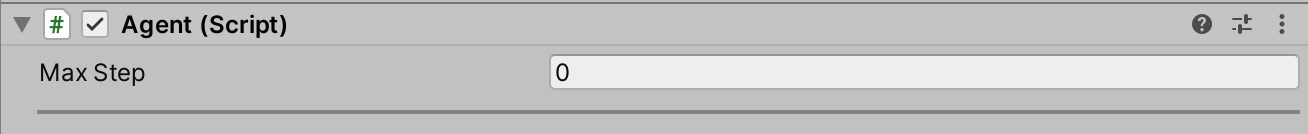
\includegraphics[scale=0.5]{img/agent_komponente}
  \caption{Unity ML-Agents Agenten Komponente}
  \label{fig:agent_komponente}
\end{figure}

Abbildung \ref{fig:agent_komponente} zeigt die Basiskomponente des Agenten. Die Agenten Komponente stellt alle grundlegenden Funktionen des verstärkenden Lernens bereit und implementiert die Verbindung zur Akademie und dem Verhalten des Agenten. Ohne das überschreiben der Funktionen ist die Agentenklasse jedoch ohne Funktion. Die genauen Methoden zur Implementierung eigener Agentenklassen werden näher in Kapitel \ref{subsec:programmierschnittstellen} behandelt. Das einzige Feld zur Konfiguration ist Max Step, welches die maximale Anzahl der Schritte innerhalb einer Episode festlegt.

\begin{figure}[H]
  \centering  
  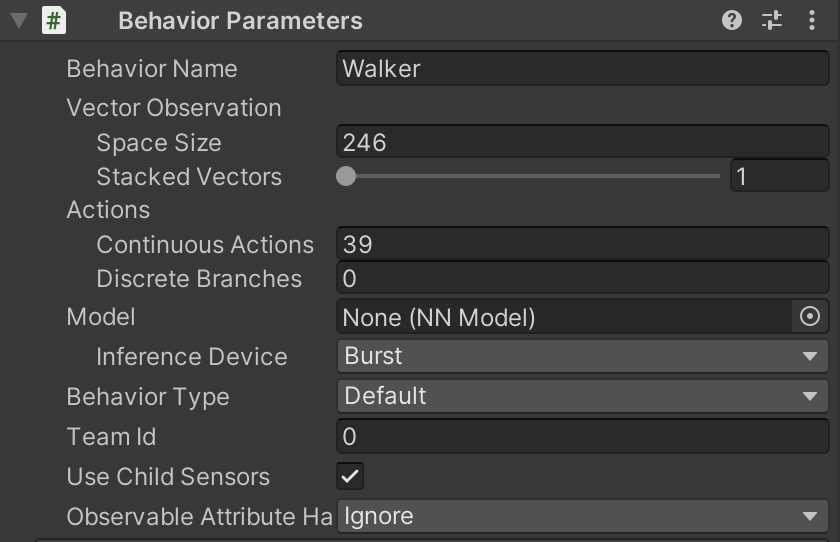
\includegraphics[scale=0.5]{img/verhalten_komponente.png}
  \caption{Unity ML-Agents Verhalten Parameter Komponente}
  \label{fig:verhalten_komponente}
\end{figure}

In Abbildung \ref{fig:entscheidung_anfragen_komponente} ist die Verhaltens Parameter Komponente zusehen. Das Verhalten legt die Ein- und Ausgangsgröße des Modells fest. Für das Training muss ein gleichnamiges Verhalten in der Konfigurationsdatei definiert sein. Um ein bereits trainiertes Verhalten zu verwenden muss im Modell Feld die Modelldatei referenziert werden.

\begin{itemize}
  \item Behaviour Name: Name des Verhaltens / wird in Trainer Konfiguration referenziert
  \item Space Size: Anzahl an Beobachtungen / Inputknoten für NN
  \item Continuous Actions: Anzahl an Aktionen / Outputknoten von NN
  \item Model: Referenz auf bereits trainiertes Modell zur Verwendung in Inferenz
  \item Behaviour Type: Lernmodus Default = Lernen, Heuristic, Inferenz
\end{itemize}

\begin{figure}[H]
  \centering  
  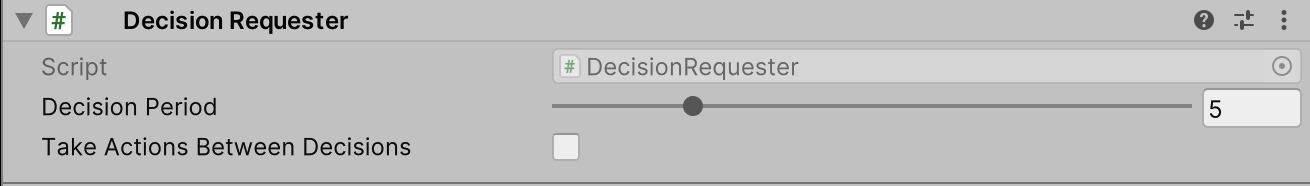
\includegraphics[scale=0.5]{img/entscheidung_anfragen_komponente.png}
  \caption{Unity ML-Agents Entscheidung Anfragen Komponente}
  \label{fig:entscheidung_anfragen_komponente}
\end{figure}

Die Komponente in Abbildung \ref{fig:entscheidung_anfragen_komponente} fragt in regelmäßigen Abständen Entscheidungen an. Das bedeutet es wird eine Beobachtung erstellt. Darauf wird die Beobachtung als Eingangswert für das neuronale Netz genutzt und dann eine Aktion vom neuronalen Netz ausgewählt. Während dem training wird diese Beobachtung zusammen mit der darauf ausgeführten Aktion und der resultierenden Belohnung im Trainingsspeicher abgelegt. Die "Decision Period" gibt an in welchem Interval der Agent eine Entscheidung treffen soll. Das "Kontrollkästchen Take Actions Between Decisions" gibt an ob der Agent die ausgewählte Aktion wiederholen soll bis die nächste Aktion ausgewählt wurde.

\subsection{Programmierschnittstellen}
\label{subsec:programmierschnittstellen}
Die Agenten Komponente enthält einige Funktionen die für das Training eines Agenten implementiert werden müssen. In den folgenden Absätzen werden die Funktionen anhand Beispielen näher erklärt.

\begin{lstlisting}[caption={Agent Funktionen},captionpos=b,label={lst:agent_funktionen}]
public override void CollectObservations(VectorSensor sensor)
{
    sensor.AddObservation(floatObservation);
}

public override void OnActionReceived(ActionBuffers actionBuffers)
{
    var continuousActions = actionBuffers.ContinuousActions;
    movement.x += continuousActions[0]
    movement.y += continuousActions[1]
}

public virtual void FixedUpdate()
{
    AddReward(floatReward);
}
\end{lstlisting}

In der CollectObservations Methoden wird festgelegt welche Daten dem Agent für das Training bereit stehen siehe Listing \ref{lst:agent_funktionen} Zeile 1-3. CollectObservations wird für jede angefragte Entscheidung ausgeführt und das Ergebnis an das NN Modell oder den Python Trainer übergeben.

Wenn eine Entscheidung angefragt wurde und das NN Modell ein Ergebnis liefert wird dieses hier von numerischen Werten in Aktionen umgewandelt. In Listing \ref{lst:agent_funktionen} Zeile 6-11 wird gezeigt wie die Aktion in x und y Bewegung umgesetzt wird.

Im Beispielcode in Listing \ref{lst:agent_funktionen} Zeile 13-16 wird ein Reward in jedem FixedUpdate vergeben über die AddReward Methode die auch Teil der Agenten-Komponente ist. Der Reward kann aber an jeder Stelle im Code vergeben werden, der Code dient hier nur als ein Beispiel.

\begin{lstlisting}[caption={Trainer Konfigurationsdatei},captionpos=b,label={lst:trainer_konfiguration}]
{
behaviors:
  Walker:
    trainer_type: ppo
    hyperparameters:
      batch_size: 2048
      buffer_size: 20480
      learning_rate: 0.0003
      beta: 0.005
      epsilon: 0.2
      lambd: 0.95
      num_epoch: 3
      learning_rate_schedule: linear
    network_settings:
      normalize: true
      hidden_units: 256
      num_layers: 3
      vis_encode_type: simple
    reward_signals:
      extrinsic:
        gamma: 0.995
        strength: 1.0
    keep_checkpoints: 5
    checkpoint_interval: 5000000
    max_steps: 30000000
    time_horizon: 1000
    summary_freq: 30000
environment_parameters:
  environment_count: 100.0
}
\end{lstlisting}

Die Trainings Konfigurationsdatei (siehe Listing \ref{lst:trainer_konfiguration}) enthält mehrere Teile. Der Hyperparameter Teil enthält die Hyperparameter des Maschinellen Lernalgorithmuses (Zeile 5-13), danach folgt der network\_settings Teil welcher die Konfiguration des Neuronalennetzes festlegt (Zeile 14-18). Anschließend folgen noch Konfigurationen für die Belohnungssignale im Bereich reward\_signals (Zeile 19-22) und Einstellungen für die Speicherung der Daten sowie der länge des Trainings (Zeile 23-27). Ganz am Ende der Konfigurationsdatei (Zeile 28-29) befinden sich noch Umgebungsparameter welche erweitert und während dem Training ausgelesen werden können.


\section{Unity Physik}
\label{sec:physik}
Unitys eingebaute Physik-Engine ermöglicht die realistische Berechnung von Kollisionen, Schwerkraft und anderen Kräften, was Entwicklern hilft, immersive und interaktive Umgebungen zu schaffen.

Die Festkörperkomponente (Rigidbody) erlaubt es, 3D-Objekte als nicht verformbare Einheiten innerhalb dieses Systems zu simulieren. Dies ist entscheidend für die Entwicklung realistischer physikalischer Interaktionen, wie z. B. das Bewegen von Objekten, die auf Kräfte, Drehmomente und Kollisionen reagieren.

\begin{figure}[H]
  \centering  
  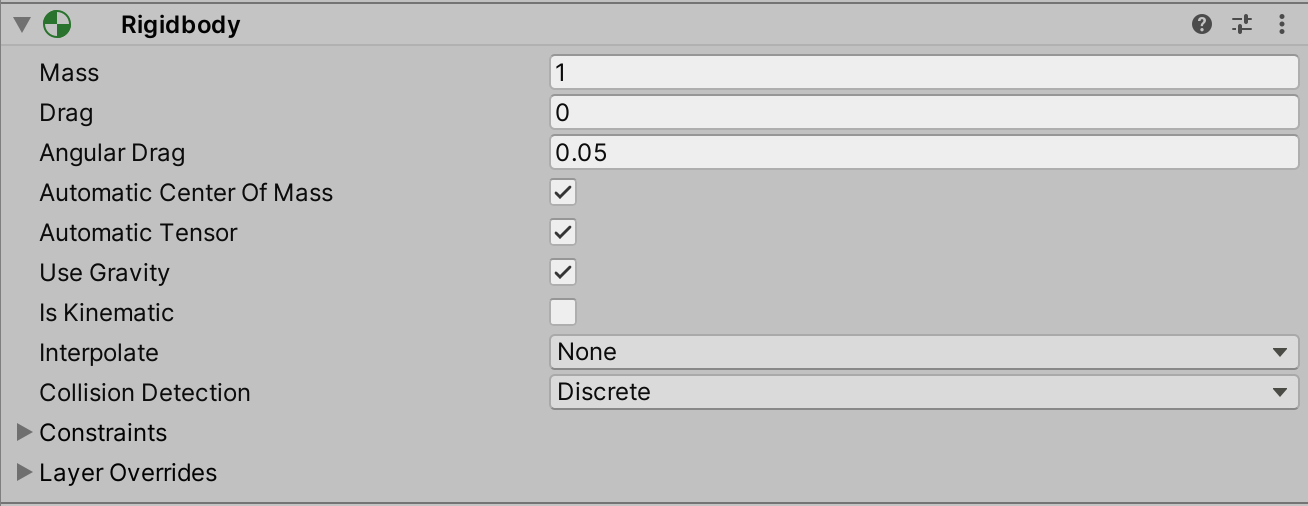
\includegraphics[scale=0.5]{img/komponente_rigidbody.png}
  \caption{Unity ML-Agents Physik Festkörper}
  \label{fig:komponente_rigidbody}
\end{figure}
\begin{itemize}
  \item Mass: gibt das Gewicht des Körpers an
  \item Drag: definiert den Geschwindigkeitsverlust eines Körpers in Bewegung durch Reibung, Luftwiederstand
  \item Angular Drag: definiert den Geschwindigkeitsverlust eines Körpers für Rotationsbewegung
  \item Collision Detection: legt fest wie Kollisionen berechnet werden (Akkurat/Leistung)
 \end{itemize}
 
Um Kollisionen zwischen Objekten zu berechnen benötigen diese zusätzlich eine Kollisionskomponente. Komplexe 3D-Modelle können in der Kollisionsberechnung jedoch in ihrer direkten Form rechenintensiv sein. Zur Optimierung werden diese Modelle vereinfacht, indem sie durch geometrische Formen wie Kugeln, Kapseln oder Boxen dargestellt werden. Abbildung \ref{fig:komponente_collider} zeigt die Unterschiedlichen Kollisionskomponenten in Unity. Abbildung \ref{fig:charakter_mixamo_collider} zeigt wie die Kollisionkomponenten (gelbe Wireframes) genutzt werden um die Körperteile eines komplexen 3D Modells vereinfacht abzubilden.

 \begin{figure}[H]
  \centering  
  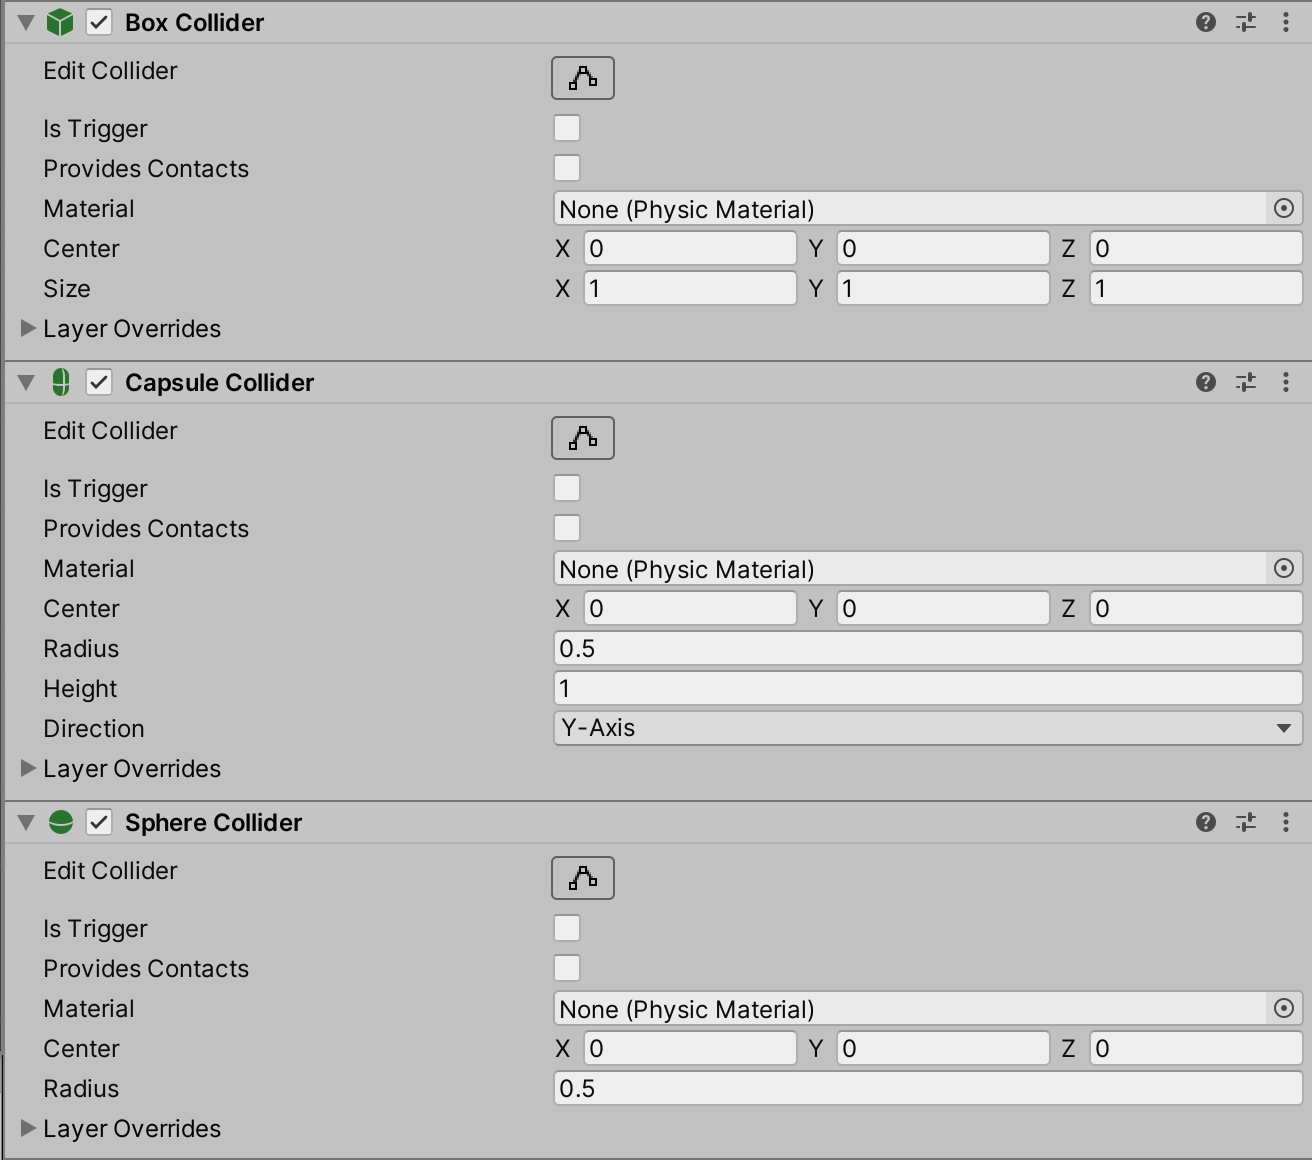
\includegraphics[scale=0.5]{img/komponente_collider.png}
  \caption{Unity ML-Agents Physik Kollisionskomponenten}
  \label{fig:komponente_collider}
\end{figure}

 \begin{figure}[H]
  \centering  
  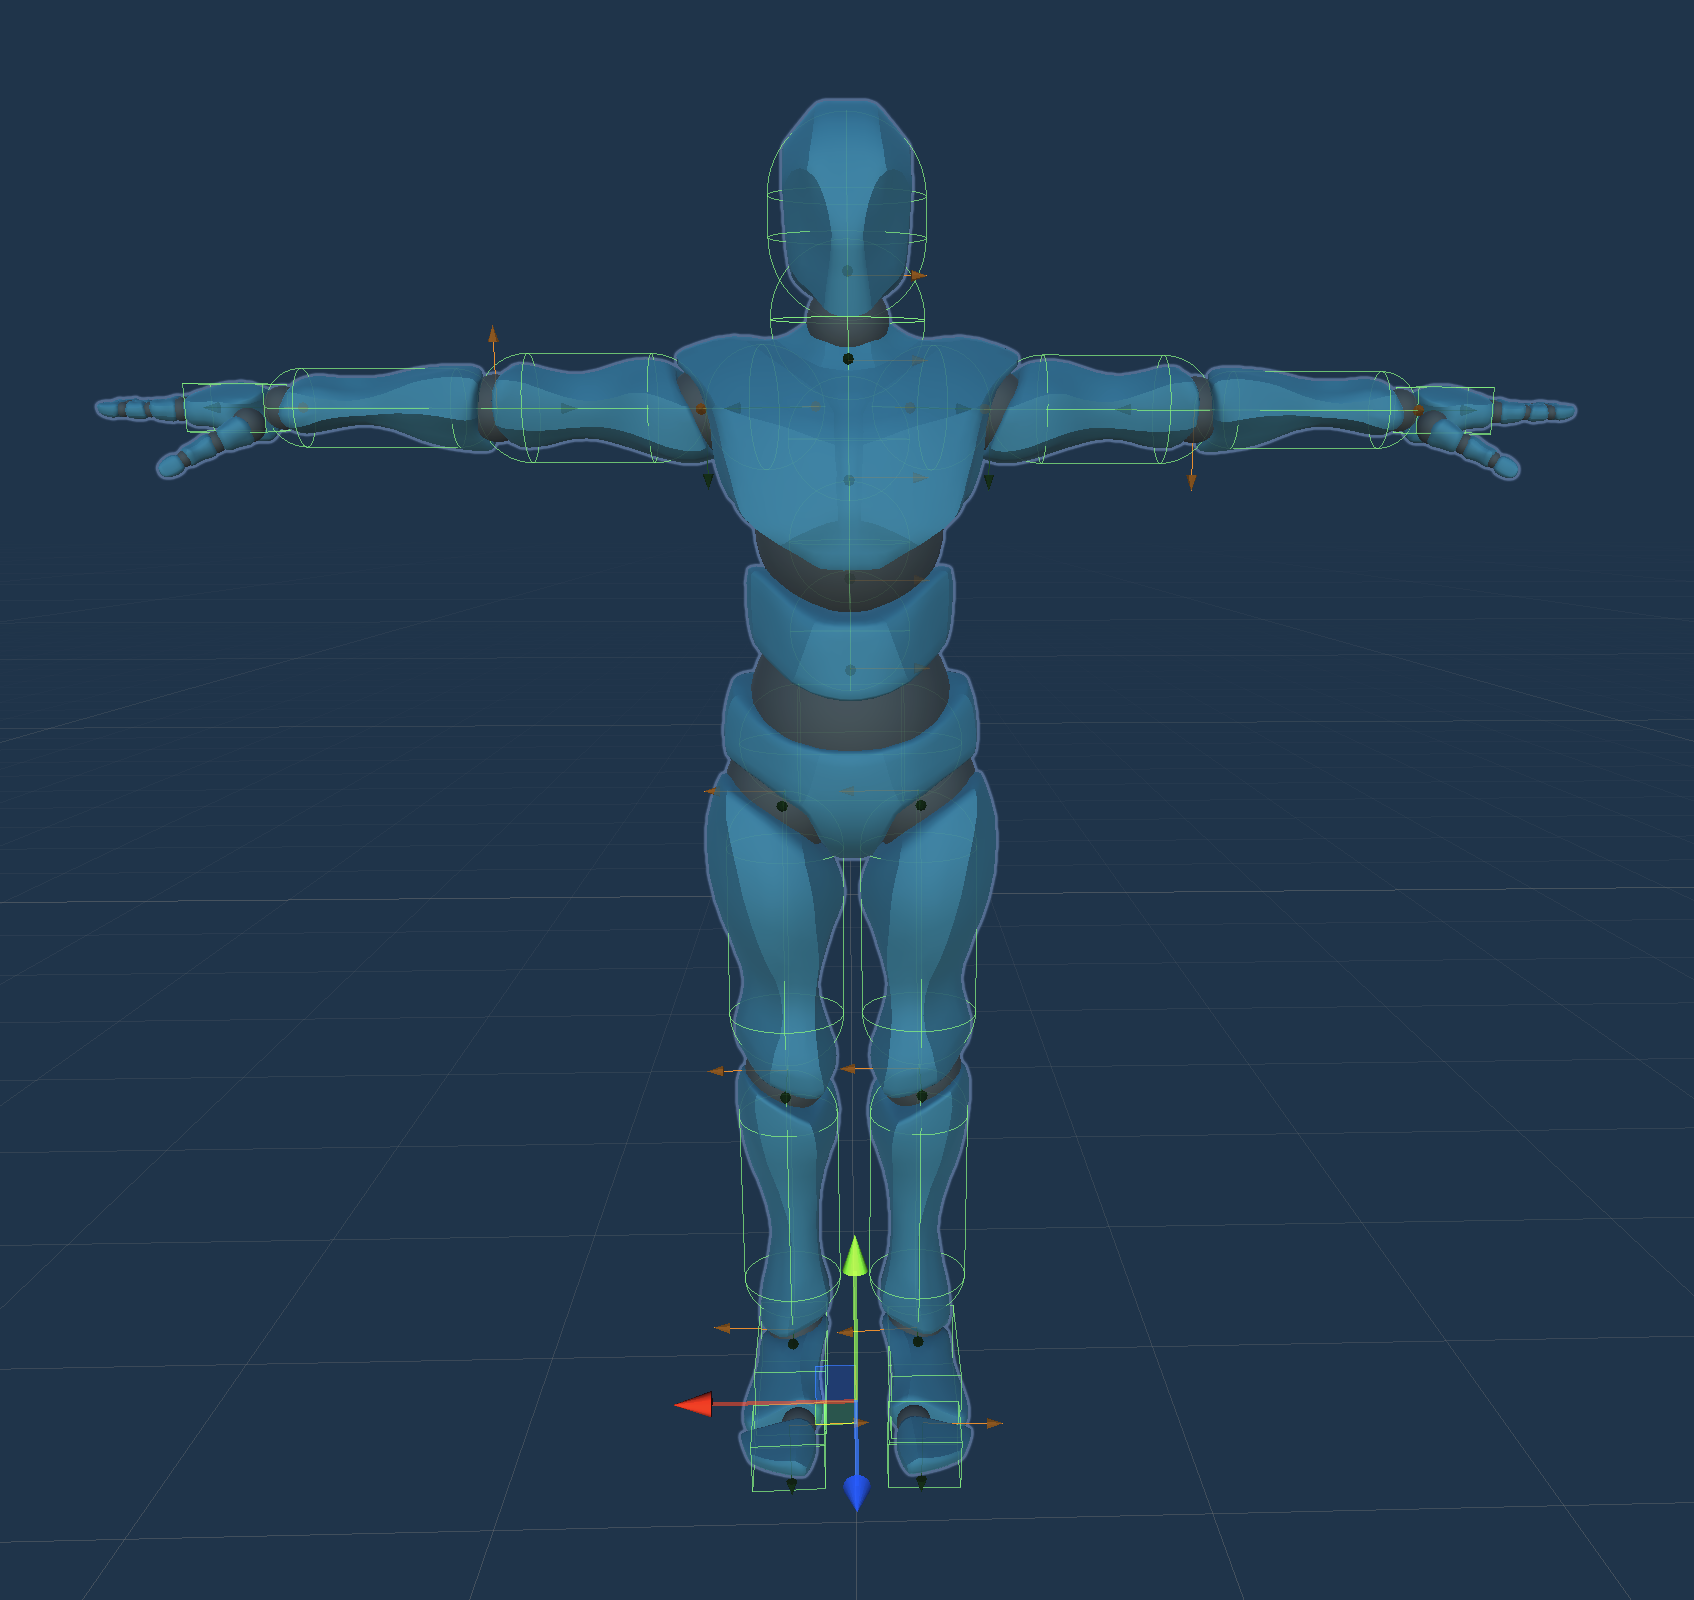
\includegraphics[scale=0.4]{img/charakter_mixamo_collider.png}
  \caption{Unity ML-Agents Physik Charakter vereinfacht mit Kollisionskomponenten }
  \label{fig:charakter_mixamo_collider}
\end{figure}

Festkörper können mit Gelenken zu komplexeren Körperstrukturen verbunden werden. Die Konfigurierbare Gelenkkomponente (Configurable Joint) ermöglicht die Simulation von Gelenken mit freier Bewegung und Rotation auf allen drei Achsen. Dies ist wesentlich, um realistische Animationen und Interaktionen in Softwaresimulationen zu erzeugen. Im Kontext dieser Arbeit wird das Gelenk auf Rotation beschränkt und als kugelförmiges Gelenk verwendet. Die Gelenke einer humanoiden Figur können somit vereinfacht aber ausreichend genau simuliert werden.

\begin{figure}[H]
  \centering
  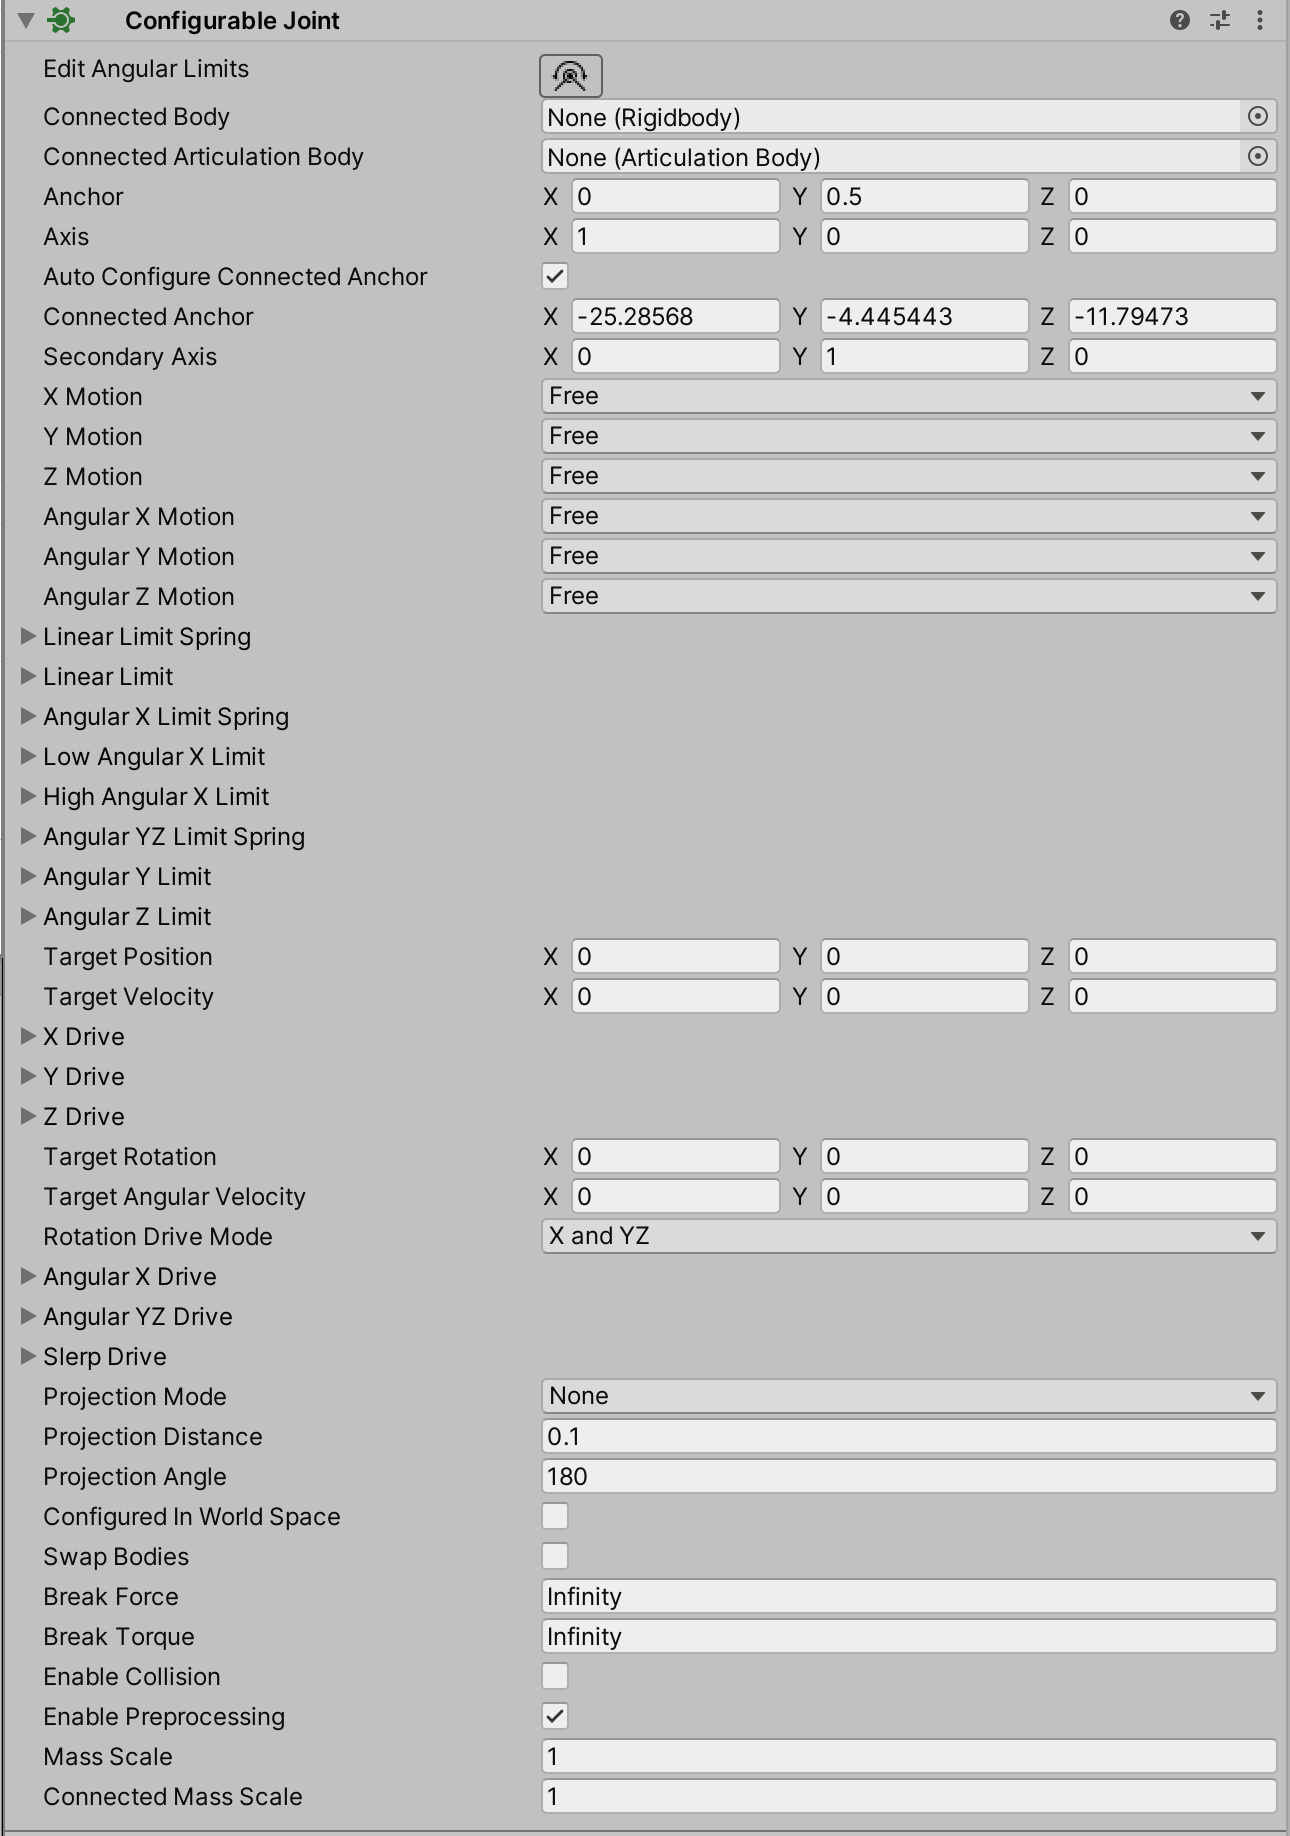
\includegraphics[scale=0.5]{img/komponente_configurable_joint.png}
  \caption{Unity ML-Agents Physik Gelenk}
  \label{fig:komponente_configurable_joint}
\end{figure}
\begin{itemize}
  \item Connected Body: bestimmt, mit welchem Körper das Gelenke verbunden ist
  \item Anchor: legt fest, an welchem Punkt die Verbindung zum verbundenen Körper besteht
  \item Axis: legt die Hauptbewegungs- und Rotationsachse fest
  \item Secondary Axis: legt die sekundäre Beweungs- und Rotationsachse fest
  \item Angular X Y Z Motion: bestimmt, ob das Gelenk Rotation zwischen den Körpern auf der X Y Z Achse zulässt
  \item Target Position: bestimmt das Ziel, zu welchem das Gelenk sich bewegen soll
  \item Angular X Y Z Limit: ermöglicht das Festlegen von Winkellimits für die Rotationsbewegungen
  \item X Y Z  und Slerp Drive: bestimmen die Stärke der Federkraft welche das Gelenk in die Zielposition bewegt
\end{itemize}
\chapter{Analyse}
\label{sec:analyse}
Zusätzlich zu den maschinellen Lernkomponenten stellt Unity auch Demonstrationsumgebungen bereit, in denen verschiedene Lösungen für gängige Verstärkungslernprobleme implementiert sind. In der Walker-Demo wird ein physisch simulierter Charakter darauf trainiert, zu einem Zielwürfel zu laufen. Sie implementiert bereits einige grundlegende Steuerungsmechanismen, die erforderlich sind, um einen Charakter in einer dynamischen Umgebung zu bewegen und zu kontrollieren. Aus diesem Grund wird in dieser Arbeit die Walker-Demo als Basis für die Entwicklung genutzt. 

In diesem Kapitel wird daher die Walker-Demo analysiert, um in den folgenden Kapiteln darauf aufzubauen. Es wird untersucht wie die Szene und der Charakter aufgebaut sind, welche Beobachtungen als Eingabe verwendet werden und wie Ausgabe des neuronalen Netz in der Umgebung ausgeführt werden. Anschließend wird der Ablauf und die verwendete Belohnungsfunktion analysiert.

\section{Szenenaufbau}
Die Szene besteht aus einem quadratischen Spielfeld mit einem Boden und Wänden, die der Charakter nicht verlassen kann (siehe Abbildung \ref{fig:walker_aufbau}). Diese Begrenzungen dienen dazu, die Bewegung des Charakters zu kontrollieren und sicherzustellen, dass die Lernumgebung konsistent bleibt. Die Umgebung umfasst weiterhin den Läufer und das Ziel, zu dem der Läufer lernt zu laufen.

\begin{figure}[H]
  \centering  
  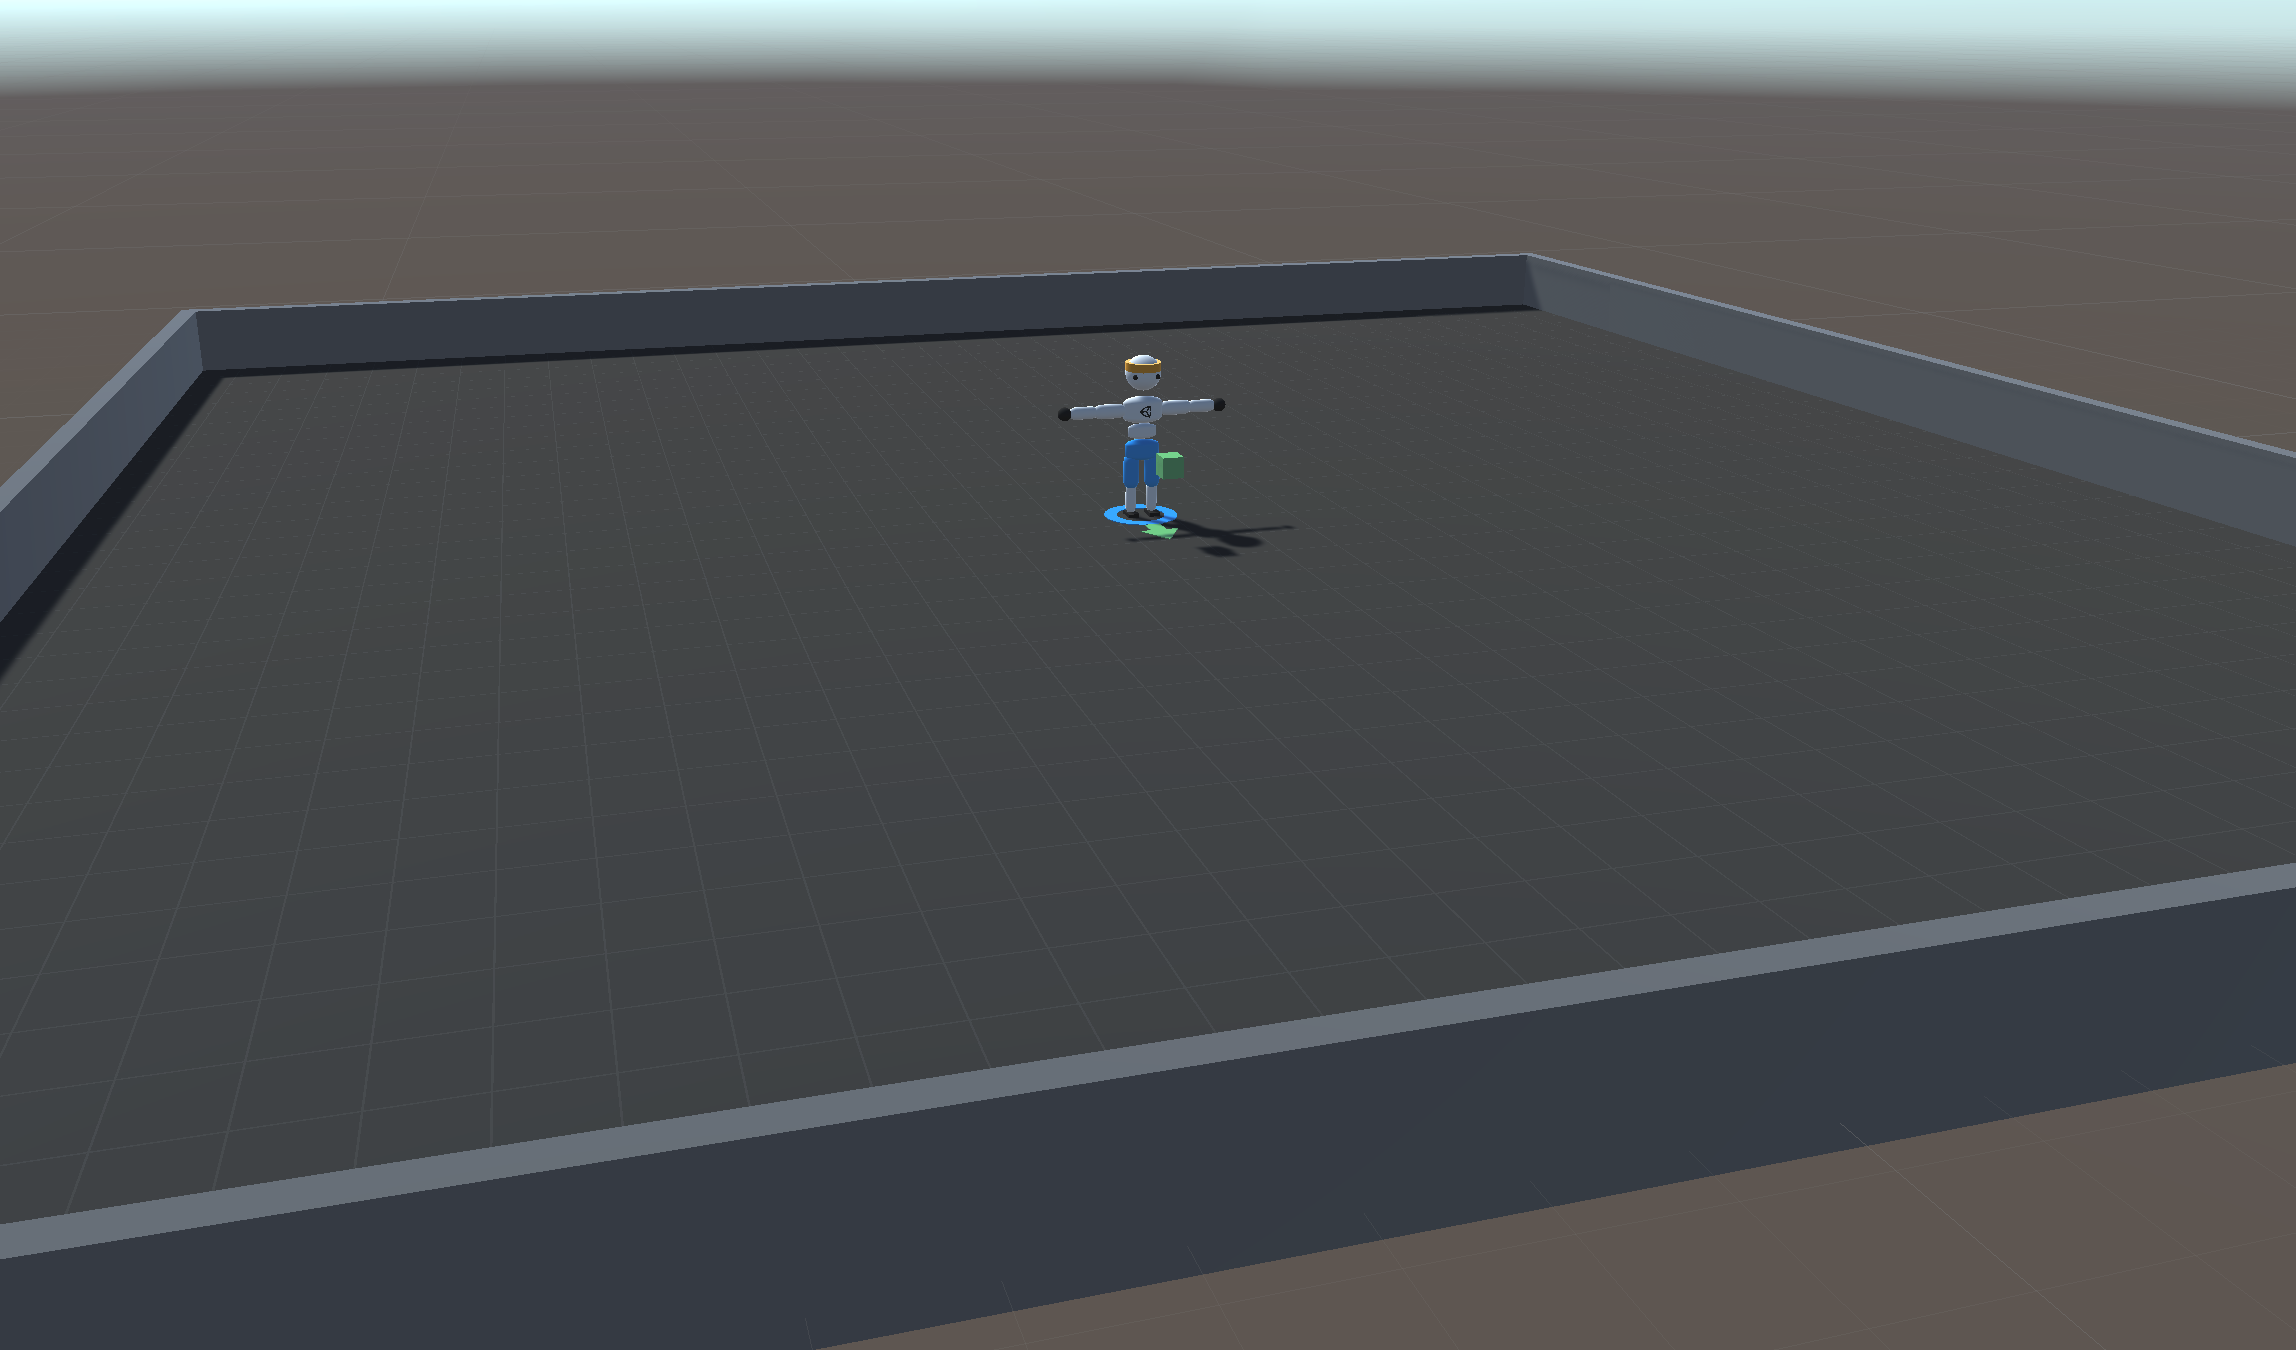
\includegraphics[scale=0.35]{img/walker_aufbau.png}
  \caption{Walker-Demo Szenenaufbau}
  \label{fig:walker_aufbau}
\end{figure}

\section{Läufer}
Der Körper des Läufers ist sorgfältig mit verschiedenen geometrischen Formen aufgebaut: 11 Kapseln, drei Kugeln und zwei Quadern. Jede dieser Formen verfügt über eine Festkörper- und eine Kollisions-Physikkomponente, die eine realistische Interaktion innerhalb der Szene ermöglichen. Die Gelenke zwischen den Körperteilen werden als Kugelgelenke simuliert, um eine flexible und natürliche Bewegung zu gewährleisten.

Die genaue Physikkonfiguration der Körperteile wird in der Tabelle \ref{table:walker_körperteile} veranschaulicht. Diese Konfiguration spielt eine zentrale Rolle, da sie die Art und Weise bestimmt, wie der Läufer lernt, auf das Ziel zuzulaufen, und dabei die physischen Einschränkungen und Möglichkeiten berücksichtigt.

\begin{table}[H]
  \centering
  {\rowcolors{1}{gray!10}{white}
  \begin{tabular}{ |p{3cm}|p{3cm}|p{2cm}|p{4cm}|p{2cm}| }
  \hline
  \textbf{Körpertei}l& \textbf{Verbundenes Körperteil} & \textbf{Gewicht} & \textbf{Winkellimits} & \textbf{Form} \\
  \hline
  Hüfte & - & 15kg & - & Kapsel \\
  \hline
  Wirbelsäule & Hüfte & 10kg & x(-20,20) y(-20,20) z(-15,15) & Kapsel \\
  \hline
  Oberkörper & Wirbelsäule & 8kg & x(-20,20) y(-20,20) z(-15,15) & Kapsel \\
  \hline
  Kopf & Oberkörper & 6kg & x(-30,10) y(-20,20) & Kugel \\
  \hline
  Oberarm LR & Oberkörper & je 4kg & x(-60,120) y(-100,100) & Kapsel \\
  \hline
  Unterarm LR & Oberarm & je 3kg & x(0,160) & Kapsel \\
  \hline
  Hand LR & Unterarm & je 2kg & - & Kugel \\
  \hline
  Oberschenkel LR & Hüfte & je 14kg& x(-90,60) y(-40,40) & Kapsel \\
  \hline
  Unterschenkel LR & Oberschenkel & je 7kg &  x(0,120) & Kapsel \\
  \hline
  Fuß LR & Unterschenkel & je 5kg & x(-20,20 y(-20,20) z(-20,20) & Quader \\
  \hline
  \end{tabular}}
  \caption{Walker Agent Körperteile}
  \label{table:walker_körperteile}
\end{table}

Der Läufer wird über die Gelenk Motor Steuerung (Joint Drive Controller) gesteuert. Das Walker Agent Skript registriert die Körperteile bei der Initialisierung in der Gelenk Motor Steuerung, wodurch eine effektive Schnittstelle zur Kontrolle der Gelenke geschaffen wird. Anschließend können über die Gelenk Motor Steuerung die Zielrotationen sowie die Maximale Kraft des Gelenks festgelegt werden, und somit der Läufer gesteuert werden. Die Gelenk Motor Einstellungen (Joint Drive Settings) siehe Abbildung \ref{fig:agent_konfiguration} \hl{bestimmen die Stärke mit welcher die Gelenke in die Zielstellung bewegt werden.}

\begin{figure}[H]
  \centering  
  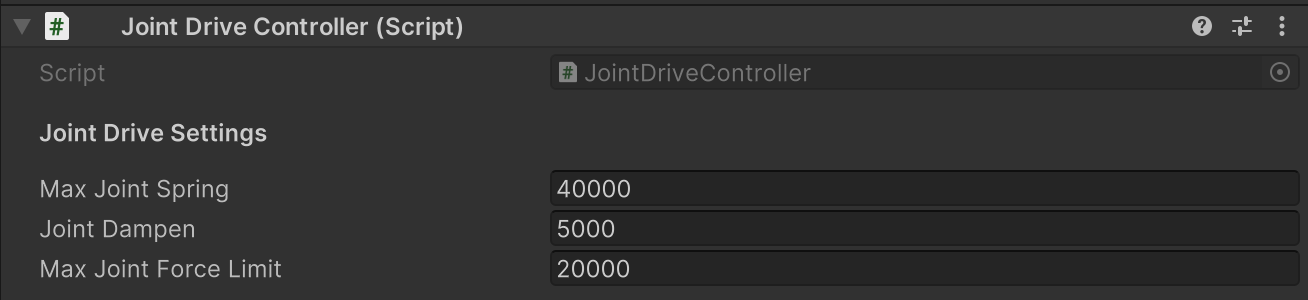
\includegraphics[scale=0.5]{img/gelenk_motor_steuerung.png}
  \caption{Gelenk Motor Steuerung}
  \label{fig:gelenk_motor_steuerung}
\end{figure}

\begin{itemize}
  \item Max Joint Spring: Bestimmt den Drehmoment mit welchem das Gelenk in die Zielposition rotiert wird.
  \item Joint Dampen: Verringert den Drehmoment proportional zur Differenz zwischen aktueller Geschwindigkeit und der Zielgeschwindigkeit. Verringert Schwingungen.
  \item Max Joint Force Limit: Gibt die maximale Kraft des Gelenks an (verhindert zu schnelle Bewegung bei großer Abweichung).
\end{itemize}


\section{Agent}
Das Walker Agent Skript, definiert den Läufer als Agent für das maschinelle Lernen. In Abbildung \ref{fig:agent_konfiguration} wird die Agentenkomponente im Inspektor gezeigt. Diese Komponente ist entscheidend für die Konfiguration der Lernumgebung des Läufers. Um die Komponente zu nutzen, müssen hier die Körperteile des Walkers referenziert werden. Diese Referenzierung ermöglicht es, spezifische Bewegungen und Interaktionen der einzelnen Körperteile zu steuern, was für das Training des Agenten entscheidend ist. Zusätzlich kann eine Zielgeschwindigkeit festgelegt werde und ob die Geschwindigkeit variieren soll während dem Training. Die Geschwindigkeit während dem Training zu variieren hilft dem Agent sein Verhalten besser an Umgebungsveränderungen anzupassen. Als letztes muss auch das Zielobjekt referenziert werden.

\begin{figure}[H]
  \centering  
  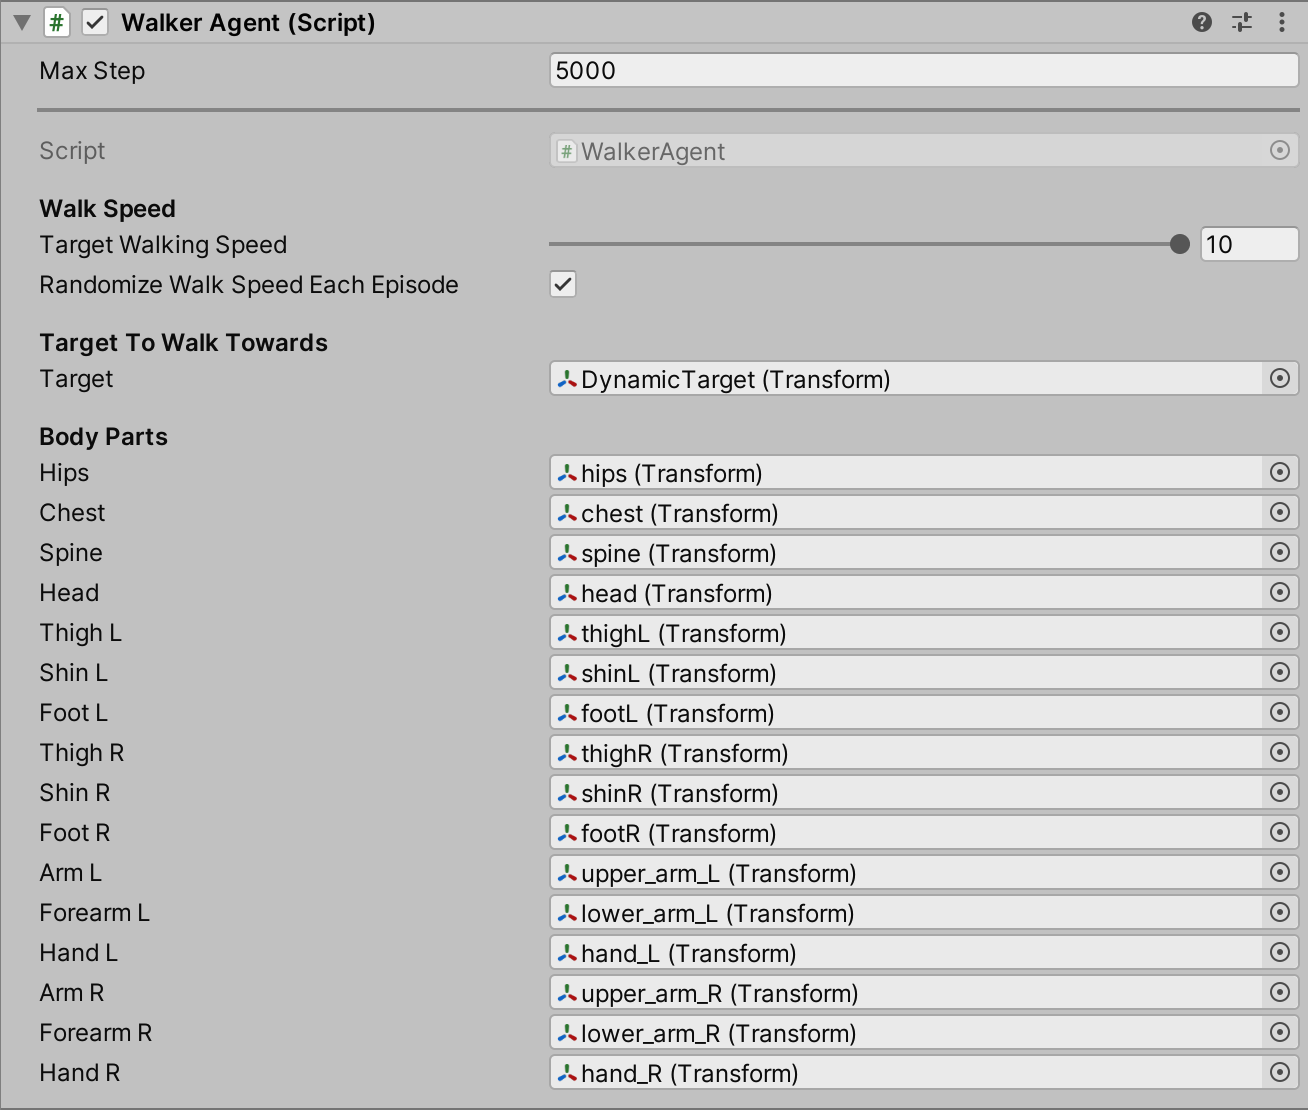
\includegraphics[scale=0.5]{img/agent_konfiguration.png}
  \caption{Agent Konfiguration}
  \label{fig:agent_konfiguration}
\end{figure}

Die Beobachtung des Agenten wird in Tabelle \ref{table:walker_beobachtung} dargestellt. Für jedes Körperteil wird die Beobachtung aus Tabelle \ref{table:walker_beobachtung_körperteil} dem Zustand angefügt. Die Beobachtungen müssen den Zustand des Läufers und der Umgebung im Bezug auf das Trainingsziel genau darstellen. Nur so kann der Agent die Situation verstehen und das Ziel erreichen.

\begin{table}[H]
  \centering
  {\rowcolors{1}{gray!10}{white}
  \begin{tabular}{ |p{1cm}|p{9cm}|p{5cm}|}
  \hline
  \textbf{ID} & \textbf{Beobachtung} & \textbf{Anmerkung}  \\
  \hline
  \rowids & Abweichung Durchschnittsgeschwindigkeit von Zielgeschwindigkeit &  \\
  \hline
  \rowids & Durchschnittsgeschwindigkeit &  \\
  \hline
  \rowids & Zielgeschwindigkeit & \\
  \hline
  \rowids & Abweichung Hüftrotation von Zielrotation & \\
  \hline
  \rowids & Abweichung Kopfrotation von Zielrotation & \\
  \hline
  \rowids & Zielposition & \\
  \hline
  \rowids & Körperteil Beobachtungen & Beobachtung aus Tabelle \ref{table:walker_beobachtung_körperteil} für jedes Körperteil \\
  \hline
  \end{tabular}}
  \caption{Walker Agent Beobachtung}
  \label{table:walker_beobachtung}
\end{table}
\rowidsclear

\begin{table}[H]
  \centering
  {\rowcolors{1}{gray!10}{white}
  \begin{tabular}{ |p{1cm}|p{9cm}|p{5cm}|}
  \hline
  \textbf{ID} & \textbf{Beobachtung} & \textbf{Anmerkung}  \\
  \hline
  \rowids & Bodenkontakt & \\
  \hline
  \rowids & Geschwindigkeit & \\
  \hline
  \rowids & Rotationsgeschwindigkeit & \\
  \hline
  \rowids & Position relativ zur Hüfte & \\
  \hline
  \rowids & LokaleRotation & Fehlt für Hüfte und Hände \\
  \hline
  \rowids & Gelenkstärke & Fehlt für Hüfte und Hände \\
  \hline
  \end{tabular}}
  \caption{Walker Agent Körperteil Beobachtung}
  \label{table:walker_beobachtung_körperteil}
\end{table}
\rowidsclear

Das Format einer Aktion besteht aus den in Tabelle \ref{table:walker_aktion} aufgeführten Feldern für jedes Körperteil des Läufers, ausgenommen der Hüfte und Hände. Jedes Körperteil wird somit separat bewegt, um die Bewegungen zu optimieren und schlussendlich das Gleichgewicht zu halten und das Fortbewegen zu erlernen.

Die Hüfte ist das zentrale Körperteil woran alle weiteren Körperteile mit Gelenken direkt oder indirekt anknüpfen. Aufgrund dieser zentralen Rolle wird die Hüftbeugung über das Gelenk des verbundenen Körpers gesteuert.

Da die Hände kaum Relevanz für das laufen haben, sind in der Demo fest mit dem Unterarm verbunden und brauchen daher nicht gesteuert werden.

\begin{table}[H]
  \centering
  {\rowcolors{1}{gray!10}{white}
  \begin{tabular}{ |p{1cm}|p{9cm}|p{5cm}|}
  \hline
  \textbf{ID} & \textbf{Beobachtung} & \textbf{Anmerkung}  \\
  \hline
  \rowids & Rotationswinkel X & Nur wenn Körperteil X Rotation beweglich ist\\
  \hline
  \rowids & Rotationswinkel Y & Nur wenn Körperteil Y Rotation beweglich ist\\
  \hline
  \rowids & Rotationswinkel Z & Nur wenn Körperteil Z Rotation beweglich ist\\
  \hline
  \rowids & Gelenkstärke & \\
  \hline
  \end{tabular}}
  \caption{Walker Agent Aktion}
  \label{table:walker_aktion}
\end{table}
\rowidsclear

Die Belohnungsfunktion enthält zwei Komponenten. Zum einen wird die Differenz der Bewegung in Zielrichtung zwischen momentaner Bewegung und Zielbewegung durch die Funktion $R_V$ bewertet. Somit wird der Läufer dazu motiviert effizient auf das Ziel zuzusteuern, indem Geschwindigkeit und Richtung optimiert werden. Zum Anderen wird die Abweichung zwischen momentaner Blickrichtung und der Zielrichtung in $R_L$ berechnet. Diese Komponente stellt sicher das der Läufer sich vorwärts geradeaus auf das Ziel bewegt. Die Belohnung ergibt sich am ende durch die Multiplikation beider Teilterme. Die Verwendung der Multiplikation hat zur Folge das die Belohnung gleichermaßen von beiden Teiltermen abhängig ist und es somit notwendig ist, beide Teile gleichzeitig zu optimieren. Als Ergebnis lernt der Läufer gleichermaßen die Ausrichtung als auch die Bewegung in Zielrichtung.

\begin{figure}[H]
  \centering  
  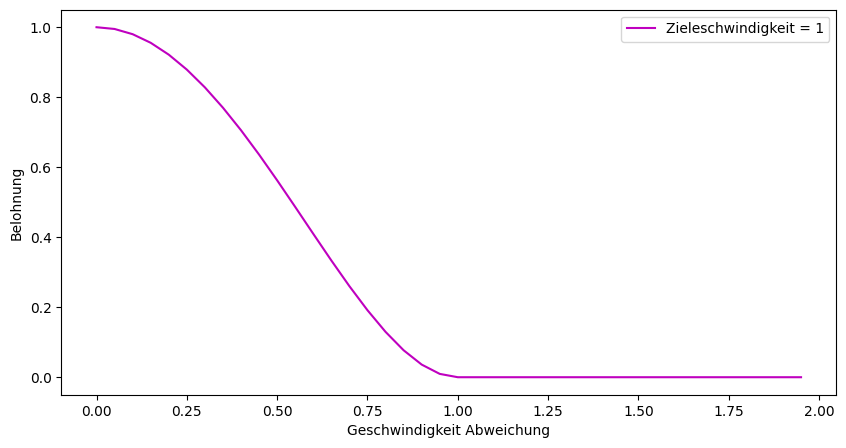
\includegraphics[scale=0.5]{img/match_velocity_demo_vel1.png}
  \caption{Walker Demo Match Velocity Belohnungsfunktion}
  \label{fig:match_velocity_demo_vel1}
\end{figure}

$V_\delta=Clip(|\vec{Geschwindigkeit} - \vec{Zielgeschwindigkeit}|, 0, |\vec{Zielgeschwindigkeit}|)$ \\
$R_V=(1 - (V_\delta / |\vec{Zielgeschwindigkeit}|)^2)^2$ \\

\begin{figure}[H]
  \centering  
  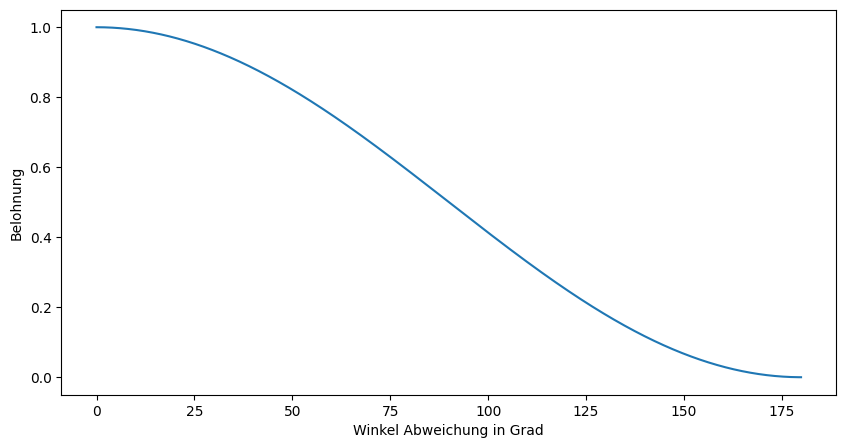
\includegraphics[scale=0.5]{img/look_at_target_demo.png}
  \caption{Walker Demo Look At Target Belohnungsfunktion}
  \label{fig:look_at_target_demo}
\end{figure}

$R_L=(\vec{Zielrichtung} \cdot \vec{Blickrichtung})+ 1) \cdot 0.5$ \\
$R=R_V \cdot R_L$

Initialisierung bzw Episodereset erklären
Orientation Object erklären
Zielsetzung erklären
Rewardfrequenz erwähnen
\chapter{Charaktercontroller}
\label{sec:charaktercontroller}
Folgender Abschnitt geht auf die Anforderungen eines Charaktercontrollers so wie die Entwicklung innerhalb dieser Arbeit ein. Dabei werden verschiedenen Ansätze getestet, implementiert und evaluiert. Die Versuche sind jeweils in Ziel, Umsetzung und Auswertung unterteilt.

\section{Nutzersteuerung}
Um von einem Charaktercontroller sprechen zu können muss der Agent über Nutzerinput gesteuert werden können. Mit diesem Gedanke wurde die ersten Anpassungen der Walker Demo implementiert um das Ziel zur Laufzeit über Tastatureingabe zu bewegen.
\begin{lstlisting}[caption={Nutzersteuerung erster Prototyp},captionpos=b,label={lst:nutzersteuerung_1}]
void FixedUpdate()
{
    //Einlesen Tastatur Input
    float inputHor = Input.GetAxis("Horizontal");
    float inputVert = Input.GetAxis("Vertical");
        
    //Setzen der Zielposition
    transform.position = root.position + root.forward * inputVert + root.right * inputHor;
}
\end{lstlisting}
Die Funktion in Listing \ref{lst:nutzersteuerung_1} liest den Input über das Unity InputSystem. Das Ziel wird relativ zur Hüfte gesetzt. Dieser Ansatz funktioniert grundsätzlich, hat aber noch ein grundlegendes Probleme und einige Einschränkungen. Das Problem ist dass die Zielposition in Abhängigkeit der Hüftrotation berechnet wird. Das hat zur folge das Schwankungen des Walkers Einfluss auf die Laufrichtung haben.

\begin{lstlisting}[caption={Nutzersteuerung berechnung mit Weltachsen},captionpos=b,label={lst:nutzersteuerung_2}]
//Setzen der Zielposition
transform.position = root.position + Vector3.forward * inputVert + Vector3.right * inputHor;
\end{lstlisting}
Durch die Nutzung der Weltachsen anstatt der Hüftrotationsachsen (siehe Listing \ref{lst:nutzersteuerung_2}) kann das Problem behoben werden. Es tritt dadurch jedoch ein weiteres Problem auf. Bei Verwendung der Weltachsen ist die Steuerung des Walkers aus Spielersicht nicht mehr intuitiv, da der Input je nach Rotation des Walkers einen anderen Einfluss hat.

Die Lösung für das Problem ist das einführen einer separaten Rotationskomponente für die Blickrichtung. Zu beginn wird die Blickrichtung mit der Vorwärtskomonente der Hüftrotation gleichgesetzt. Ausgehend von der Startrichtung wird dann über horizontalen Mausinput die Richtung angepasst (siehe Listing \ref{lst:nutzersteuerung_3}).

\begin{lstlisting}[caption={Erweiterung der Nutzersteuerung mit separater Blickrichtung},captionpos=b,label={lst:nutzersteuerung_3}]
void Start()
{
    //Root Position als Startposition festhalten
    startForward = root.forward;
    startRight = root.right;
}
void FixedUpdate()
{
    //Einlesen Tastatur Input
    float inputHor = Input.GetAxis("Horizontal");
    float inputVert = Input.GetAxis("Vertical");

    //Einlesen Maus Input
    float mouseX = Input.GetAxis("Mouse X");
    rotAngle += mouseX;

    //Berechnung der Rotation
    Quaternion rotation = Quaternion.AngleAxis(rotAngle, rotationAxis);

    //Anwendung der Rotation auf Richtungsvektoren
    Vector3 directionForward = rotation * startForward;
    Vector3 directionRight = rotation * startRight;

    //Setzen der Zielposition
    transform.position = root.position + directionForward * inputVert + directionRight * inputHor;
}
\end{lstlisting}

Mit dieser Implementierung lässt sich der Walker intuitiv steuern. Das trainierte Modell der Walker Demo beherrscht jedoch nur die Fortbewegung in Blickrichtung. Durch diese Einschränkung lässt sich von der Steuerung mit WASD nur die W Komponente nutzen. Die Vorwärtsbewegung in Kombination mit der Maussteuerung der Blickrichtung ermöglicht es sich nahezu überall hinzubewegen. Eine weitere große Einschränkung ist, das der Walker nicht darauf trainiert ist stehen zu bleiben. Das resultiert darin das der Walker fällt sobald der Nutzer keinen Tastaturinput gibt.
\section{Modell Anpassungen}
Das trainierte Modell der Walker Demo beherrscht jedoch nur die Fortbewegung in Blickrichtung. Der Läufer ist auch nicht darauf trainiert stehen zu bleiben. Das resultiert darin das der Läufer fällt sobald der Nutzer keinen Tastaturinput gibt. Dieses Kapitel beschäftigt sich mit den Einschränkungen der Walker-Demonstration im Bezug auf unterschiedliche Bewegungsrichtungen.

Im ersten Schritt wird getestet wie der Walker angepasst werden kann um die fehlenden Bewegungsabläufe in separaten Modellen zu erlernen.

\subsection{Versuch 4}
Versuch 4 behandelt die Bewegung auf der Stelle stehen. Für das stehenbleiben wird die Zielgeschwindigkeit auf 0 gesetzt während das Ziel auf der Startposition befindet. Die Belohnungsfunktion der Demo, wird ab jetzt Demo Belohnungsfunktion genannt. Die Demo Belohnungsfunktion hat das Problem das durch die Zielgeschwindigkeit geteilt wird, was bei einer Zielgeschwindigkeit von 0 zu Mathematischen Fehlern führt. Um das zu vermeiden wurde das trainieren mit einer anderen Belohnungsfunktion getestet.
\begin{figure}[H]
  \centering  
  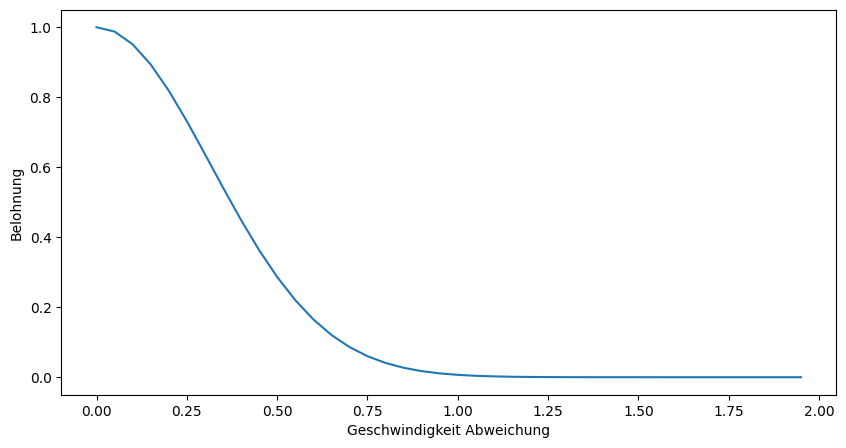
\includegraphics[scale=0.5]{img/match_velocity_exp.png}
  \caption{DeepMimic Match Velocity Belohnungsfunktion}
  \label{fig:match_velocity_exp}
\end{figure}
Die neue Belohnungsfunktion ist inspiriert von den Belohnungsfunktionen des Papers \grqq{}DeepMimic: Example-Guided Deep Reinforcement Learning of Physics-Based Character Skills\grqq{}.\cite{peng2018deepmimic}
Die Belohnungsfunktion aus Abbildung \ref{fig:match_velocity_exp} wird daher ab hier DeepMimic Belohnungsfunktion genannt.

\begin{figure}[H]
  \centering  
  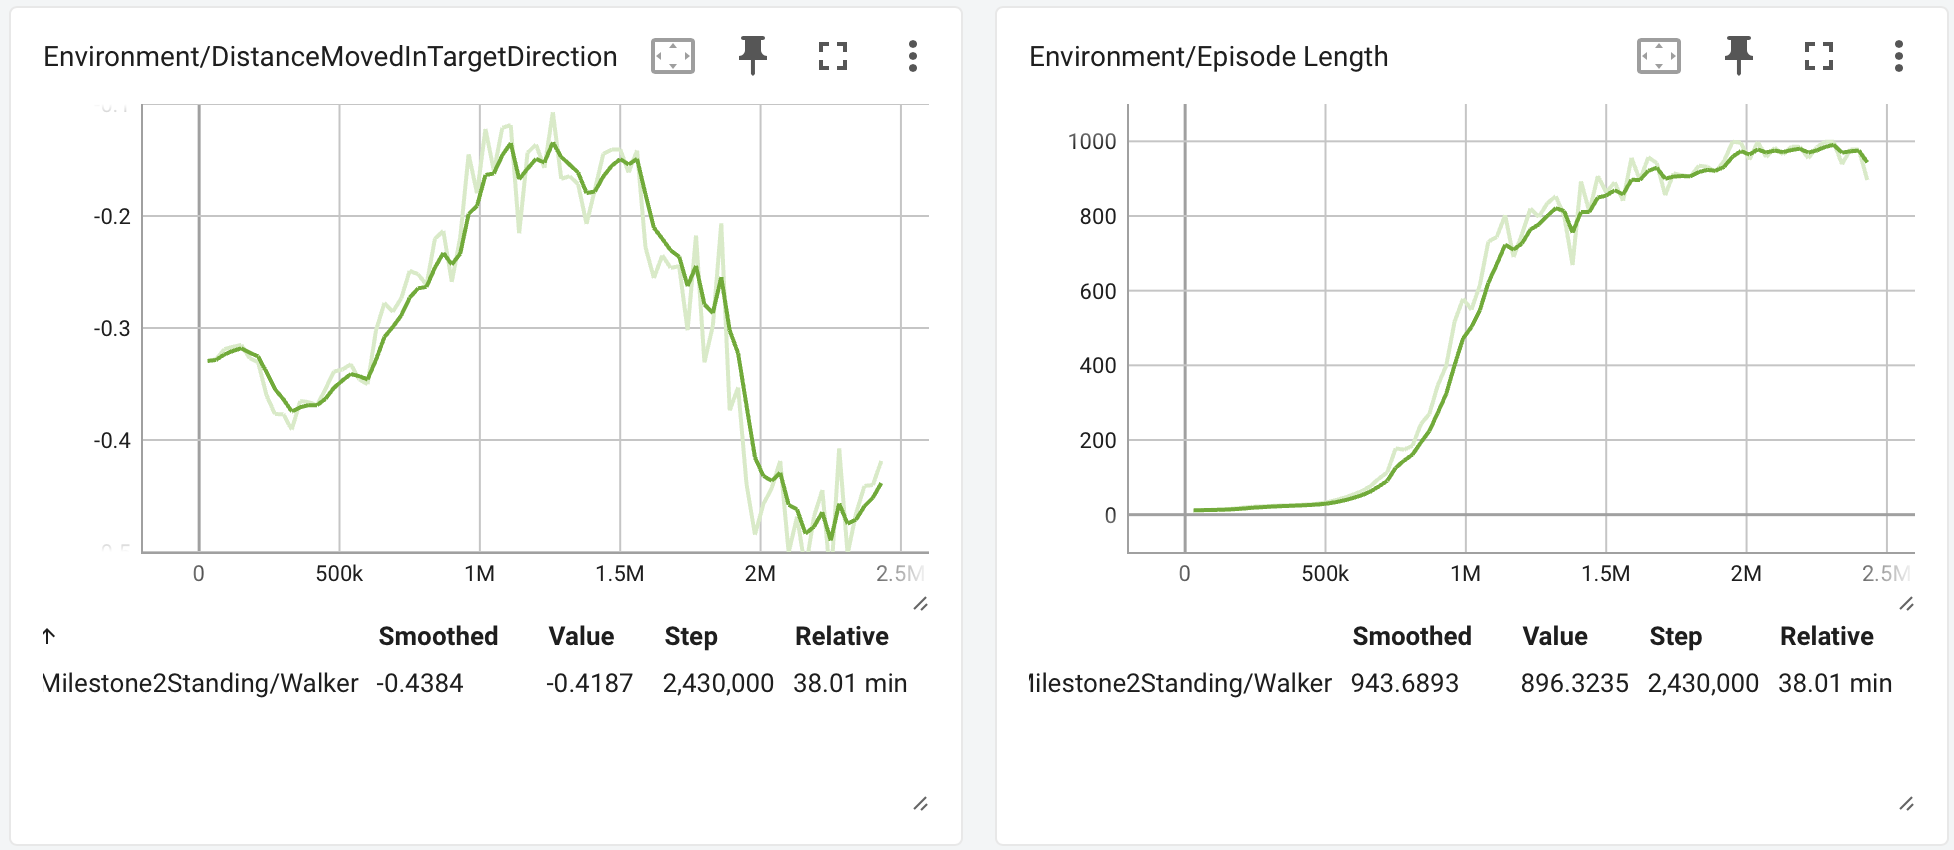
\includegraphics[scale=0.5]{img/versuch4_training}
  \caption{Versuch 4 Traininggraphen}
  \label{fig:versuch4_training}
\end{figure}

\begin{figure}[H]
  \centering  
  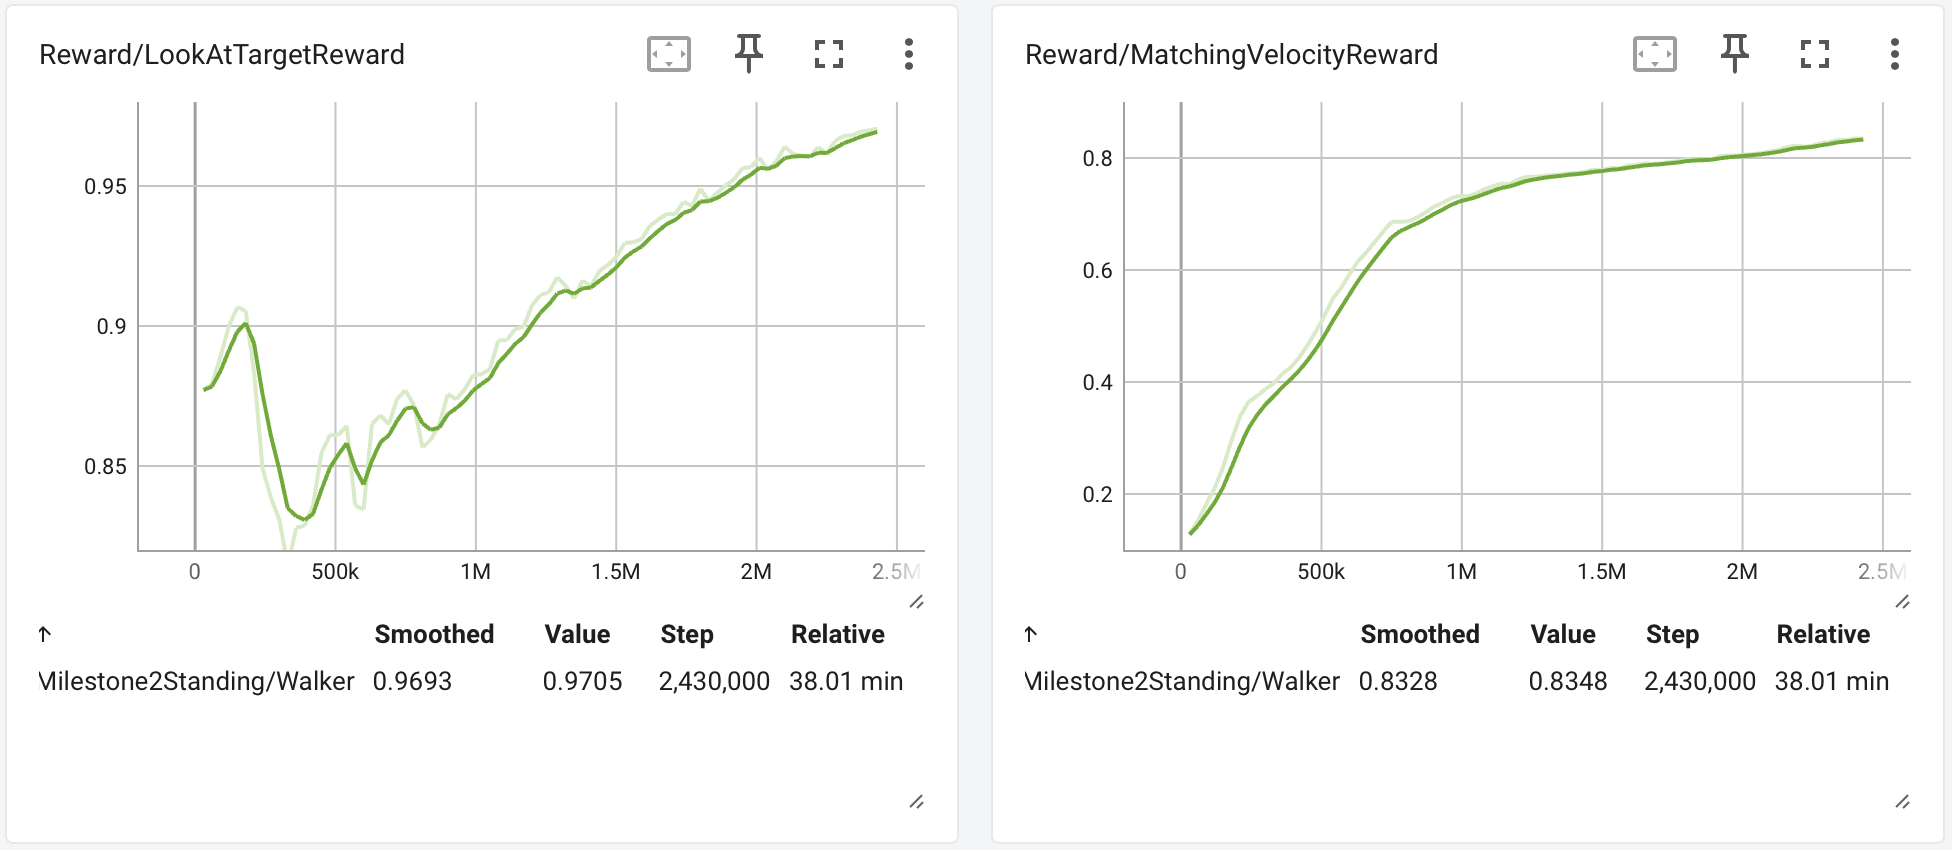
\includegraphics[scale=0.5]{img/versuch4_training_belohnung}
  \caption{Versuch4 Training Belohnungsgraphen}
  \label{fig:versuch4_training_belohnung}
\end{figure}

Der Walker konnte mit der DeepMimic Belohnungsfunktion lernen auf der Stelle zu stehen.  Abbildung \ref{fig:versuch4_training} zeigt wie die zurück gelegte Distanz um 0 herum pendelt, während die Episodenlänge die maximale Länge von 1000 erreicht hat. Die Belohnungen sind auch nahezu maximal ausgereizt siehe Abbildung \ref{fig:versuch4_training_belohnung}.

\begin{figure}[H]
  \centering  
  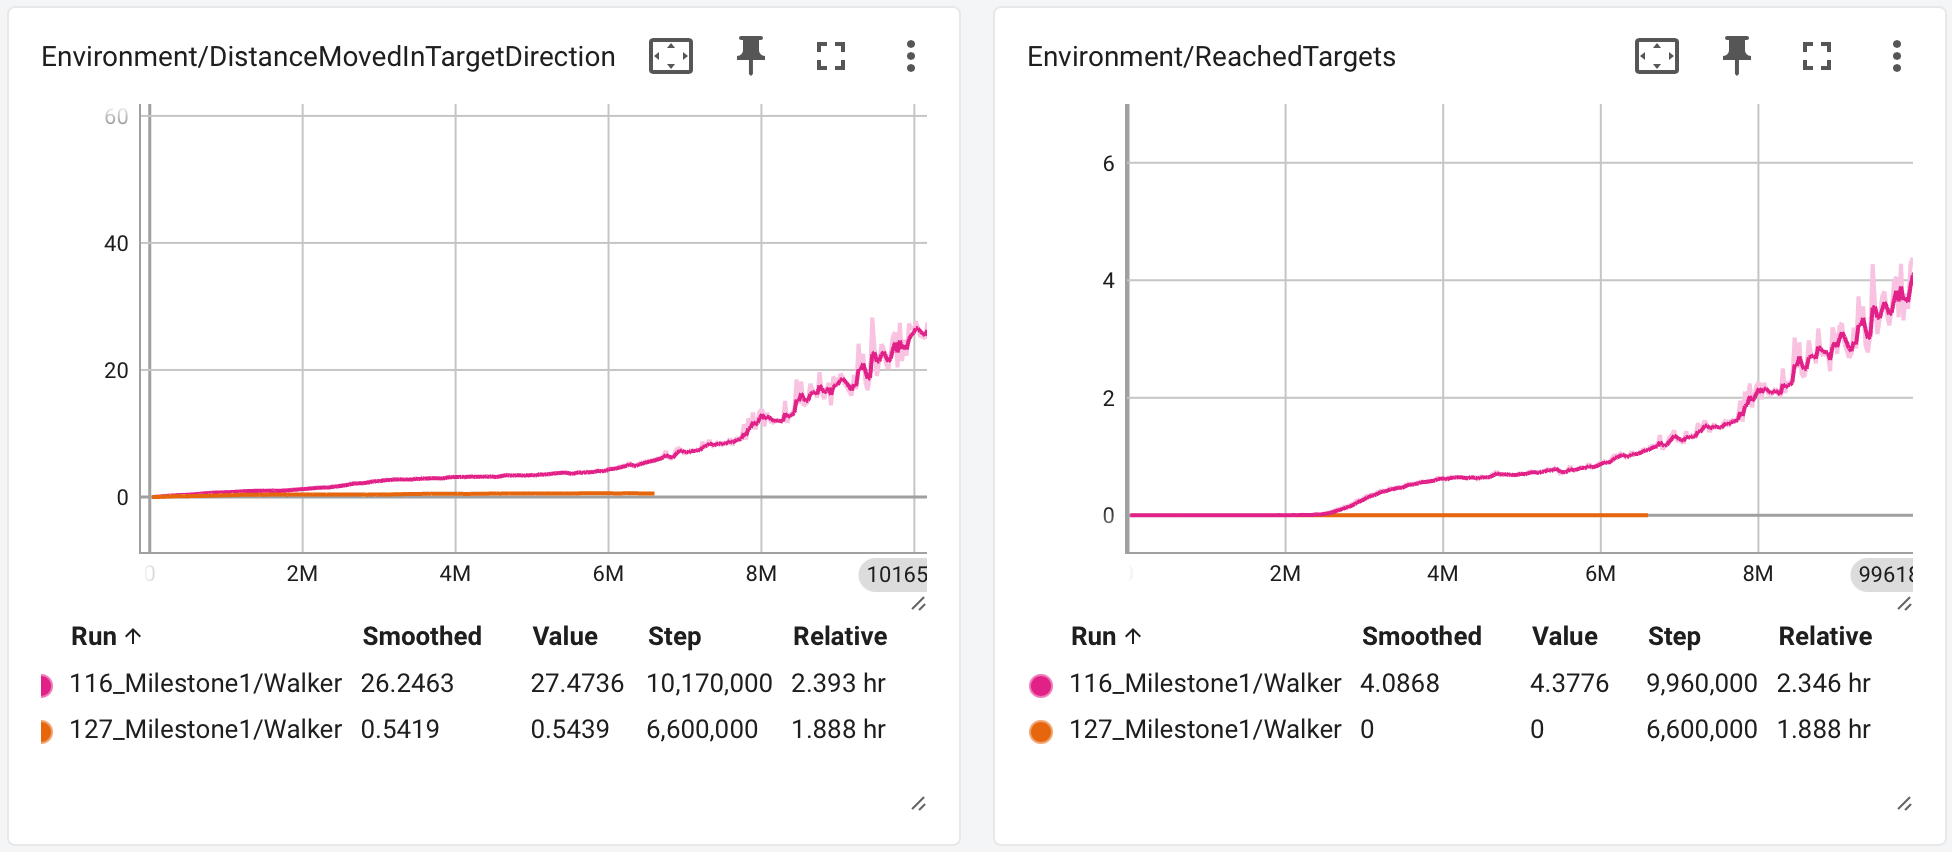
\includegraphics[scale=0.5]{img/versuch4_laufen_vergleich.png}
  \caption{Vergleich von Lauftraining mit Demo Belohnungsfunktion gegen DeepMimic Belohnungsfunktion}
  \label{fig:versuch4_laufen_vergleich}
\end{figure}

Mit zufälliger Zielgeschwindigkeit zu einem Ziel zu laufen wie im Ursprünglichen Verhalten konnte damit jedoch nicht zufriedenstellend erlernt werden. Die Abbildung \ref{fig:versuch4_laufen_vergleich} zeigt mit der orangenen Linie die Leistung der DeepMimic Belohnungsfunktion und mit der pinken Linie die Leistung der Demo Belohnungsfunktion. Nachfolgender Vergleich der Belohnungsfunktionen zeigt das die Ursprüngliche Belohnungsfunktion durch das Teilen mit der Zielgeschwindigkeit die Sensitivität der Funktion je nach Zielgeschwindigkeit beeinflusst. Daraus folgt das bei steigender Zielgeschwindigkeit eine größere Abweichung der Geschwindigkeit geduldet wird (siehe Abbildung \ref{fig:match_velocity_demo_vergleich}). Diese Anpassung verbessert die Generalisierung zwischen den wechselnden Geschwindigkeiten um ein vielfaches.

\begin{figure}[H]
  \centering  
  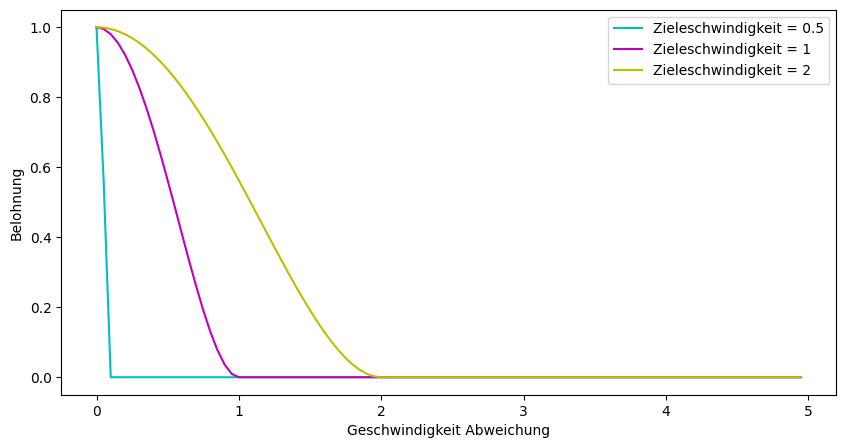
\includegraphics[scale=0.5]{img/match_velocity_demo_vergleich.png}
  \caption{Vergleich der Demo Belohnungsfunktion unter verschiedenen Zielgeschwindigkeiten}
  \label{fig:match_velocity_demo_vergleich}
\end{figure}

\subsection{Versuch 5}
Mit dieser Erkenntnis wurde eine neue Anpassung untersucht. In der folgenden Anpassung blieb die Belohnungsfunktion weitestgehend Unverändert. Lediglich das obere Limit ab welchem die Funktion eine Belohnung von 0 annimmt, wurde auf ein minimum von 0.1 beschränkt. Somit konnte sicher gestellt werden das im Bereich der normalen Fortbewegung keine Veränderung auftritt. Mit der Demo Belohnungsfunktion konnten nur Annäherungen an eine Zielgeschwindigkeit von 0 genutzt werden. Bei einer Annäherung von 0.000001 ist das Spektrum an akzeptablen Geschwindigkeiten bevor die Belohnung 0 ist nahezu unerreichbar (siehe Abbildung \ref{fig:match_velocity_vergleich_clip}). Mit dem Limit von 0.1 ist der Bereich der Belohnungsfunktion > 0 groß genug, sodass der Läufer durch ausprobieren Belohnungen über 0 erreichen kann. Somit kann der Läufer die Belohnung optimieren.\\

\begin{figure}[H]
  \centering  
  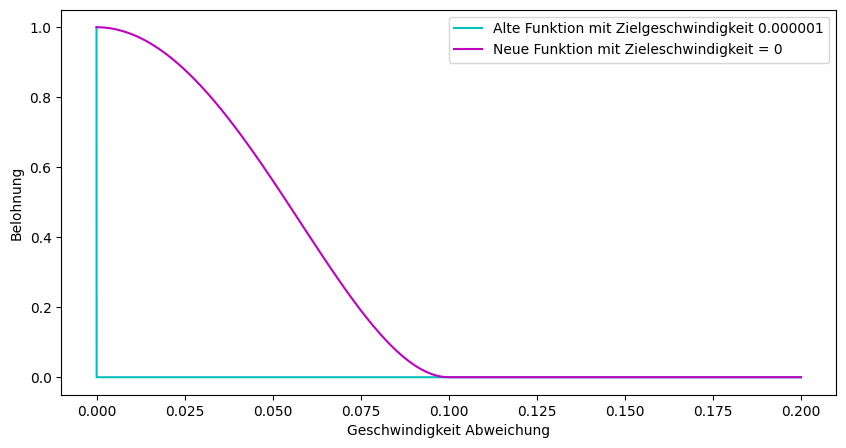
\includegraphics[scale=0.5]{img/match_velocity_vergleich_clip.png}
  \caption{Vergleich Demo gegen Belohnungsfunktion mit 0.1 Limit}
  \label{fig:match_velocity_vergleich_clip}
\end{figure}
$V_\delta=Clip(|\vec{Geschwindigkeit} - \vec{Zielgeschwindigkeit}|, 0, |\vec{Zielgeschwindigkeit}|)$ \\
$V_\delta=Clip(|\vec{Geschwindigkeit} - \vec{Zielgeschwindigkeit}|, 0, max(0.1, |\vec{Zielgeschwindigkeit}|))$ \\

Das auf einer Stelle stehen hat der Läufer damit in einem separaten Training auch erlernt. Abbildung \ref{fig:versuch5_training} zeigt das der Läufer die maximale Episoden Länge von 1000 erreicht hat ohne zu fallen. Die bewegte Distanz hat sich auch 0 angenähert.

\begin{figure}[H]
  \centering  
  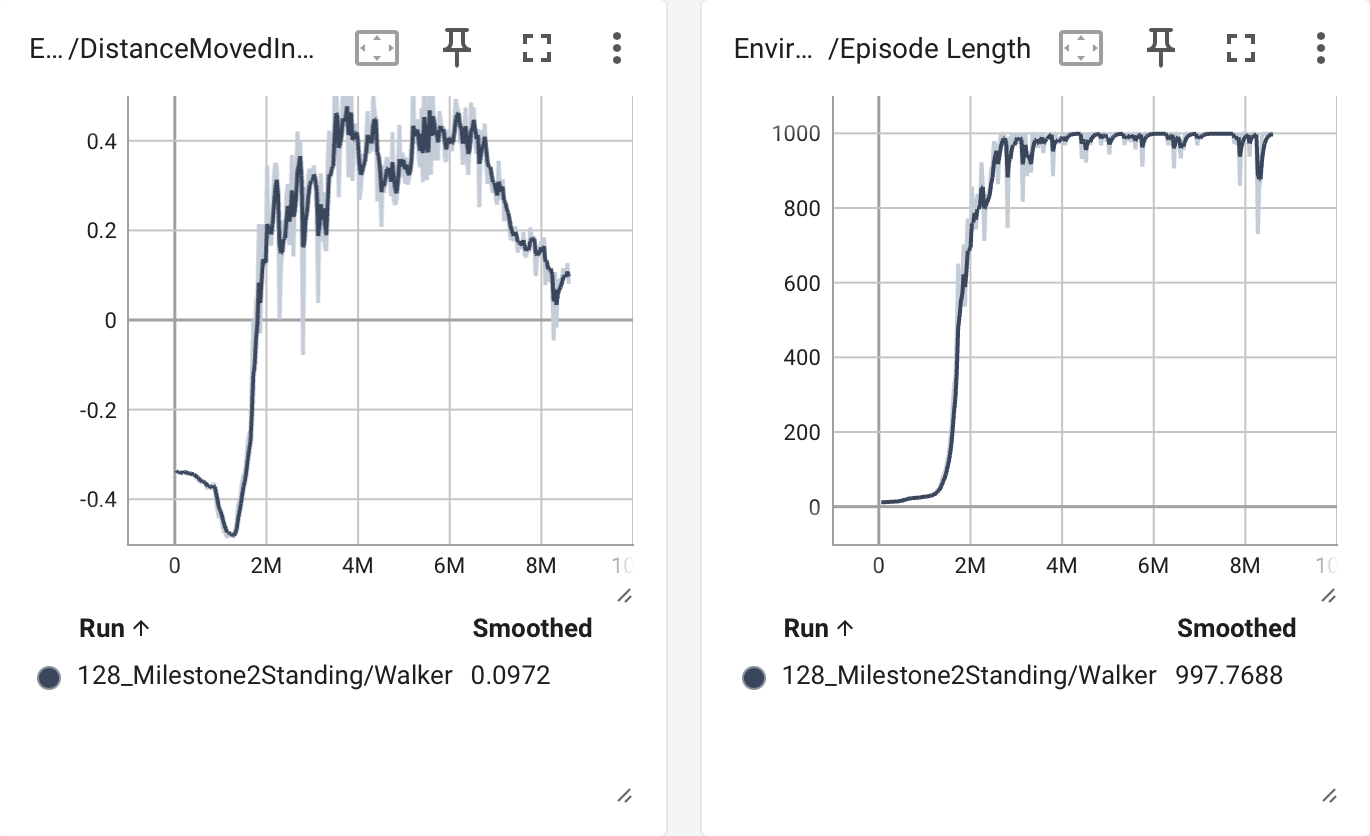
\includegraphics[scale=0.5]{img/versuch5_training.png}
  \caption{Versuch 5 Traininggraphen}
  \label{fig:versuch5_training}
\end{figure}

Die Belohnungen wurden auch weitestgehend optimiert siehe Abbildung \ref{fig:versuch5_training_belohnung}.

\begin{figure}[H]
  \centering  
  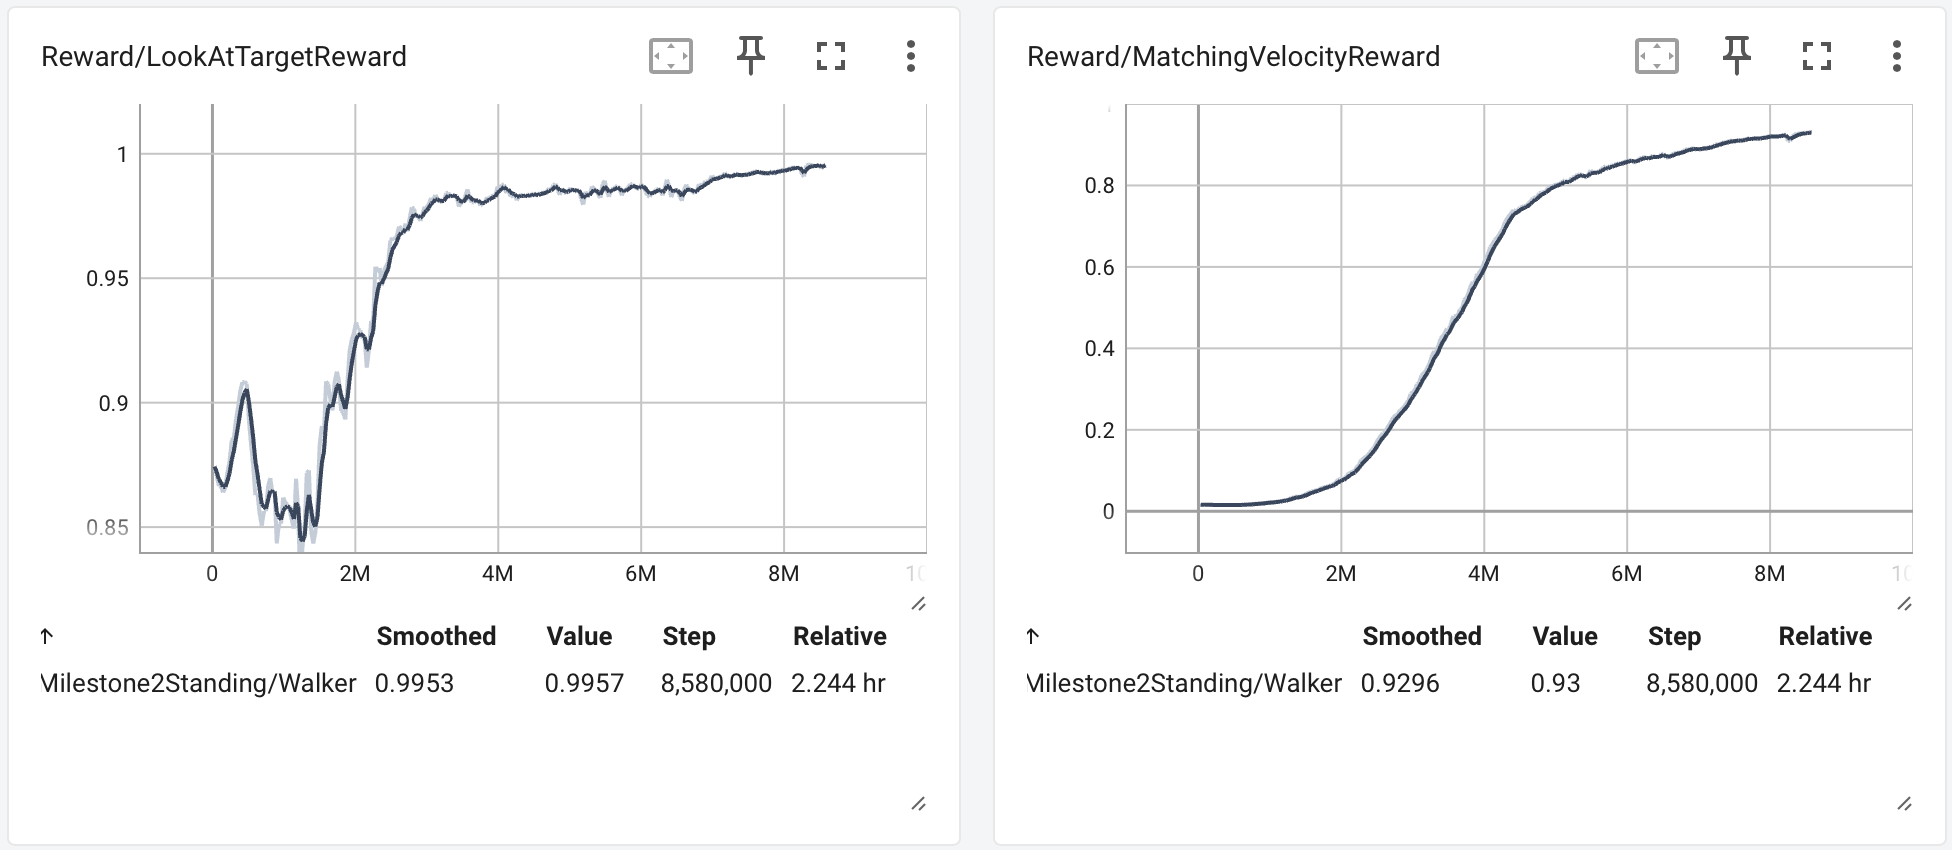
\includegraphics[scale=0.5]{img/versuch5_training_belohnung.png}
  \caption{Versuch 5 Training Belohnungsgraphen}
  \label{fig:versuch5_training_belohnung}
\end{figure}

\subsection{Versuch 6}
Der folgende Versuch untersucht das Laufen in unterschiedliche Richtungen relativ zur Blickrichtung. Um das zu realisieren wurde dem Agent ein enum mit der Laufrichtung hinzugefügt. Die Blickrichtung Belohnungsfunktion wird relativ zur Zielrichtung berechnet. Bei Vorwärtsbewegung ist die Blickrichtung gerade aus. Bei Seitlicher Bewegung ist die Blickrichtung gespiegelt zur Laufrichtung. Läuft der Läufer seitlich rechts ist die Blickrichtung links zum ziel und anders herum. Beim rückwärts gehen ist die Blickrichtung entgegen der Zielrichtung. Die Implementierung ist in \ref{lst:laufrichtung} zu sehen.

\begin{lstlisting}[caption={Laufrichtung Enum, Beobachtung und Belohnung},captionpos=b,label={lst:laufrichtung}]
public enum Direction
{
    Forward,
    Right,
    Left,
    Backward,
}
    
public override void FixedUpdate()
{
    ...
    var headForward = head.forward;
    headForward.y = 0;
    Vector3 lookDirection = cubeForward;
    switch (direction)
    {
        case Direction.Right:
            lookDirection = -walkOrientationCube.transform.right;
            break;
        case Direction.Left:
            lookDirection = walkOrientationCube.transform.right;
            break;
        case Direction.Backward:
            lookDirection = -walkOrientationCube.transform.forward;
            break;
    }
    ...
}
\end{lstlisting}

Das gehen in Zielrichtung wurde durch die Änderungen nicht beeinflusst. Separate Trainings zu den drei anderen Laufrichtungen waren erfolgreich.

\begin{figure}[H]
  \centering  
  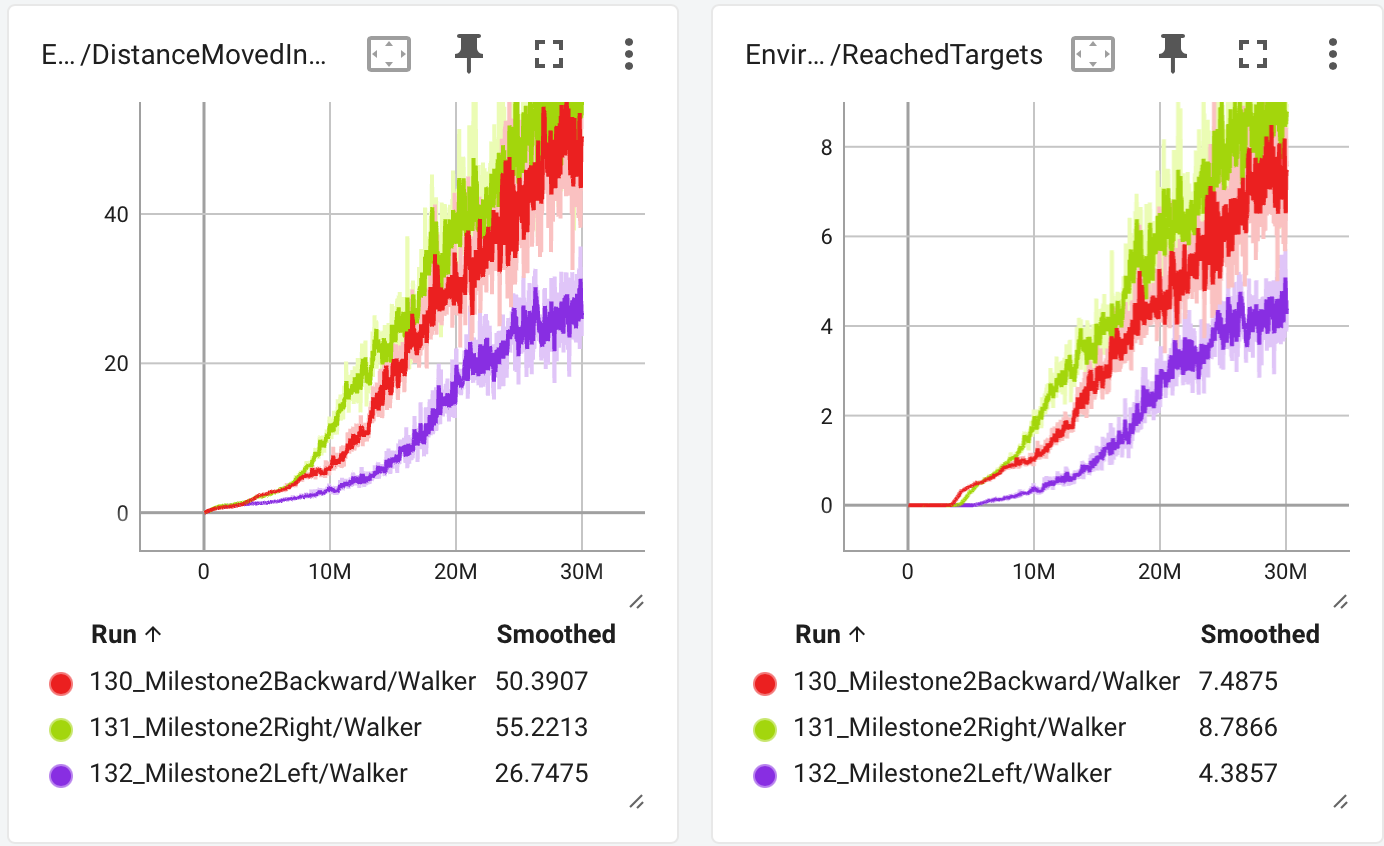
\includegraphics[scale=0.5]{img/versuch6_training.png}
  \caption{Versuch 6 Traininggraphen}
  \label{fig:versuch6_training}
\end{figure}

Abbildung \ref{fig:versuch6_training} zeigt die zurückgelegte Distanz und die Anzahl an erreichten Zielen in einer Trainingsepisode. Die Ergebnisse der 3 Laufrichtungen (rot = Rückwärts, gelb = rechts, blau = links) sind alle vergleichbar mit den Ergebnissen der Demo. Die Abweichung der Laufrichtung Links ist vermutlich der zufällligen Natur des Trainings anzurechnen.

\subsection{Versuch 7}
Die Charaktersteuerung benötigt je nach Tastatureingabe eine der vier Bewegungsrichtungen. Der Unity ML-Agents Agent enthält eine Funktion zum wechseln des verwendeten Modells. Mit dieser Funktion wird in folgender Implementierung zwischen den Modellen aus Versuch 6 gewechselt um alle Bewegungsrichtungen mit einer Steuerung abzudecken. Zu Erwarten ist das die Bewegung in die einzelnen Richtungen funktioniert, der Läufer aber beim Wechsel zwischen den Modellen das Gleichgewicht nicht halten kann.

\begin{lstlisting}[caption={Laufrichtung Modell wechseln},captionpos=b,label={lst:laufrichtung_modell_wechsel}]
public override void FixedUpdate() {
    ...    
    agent.targetWalkingSpeed = 5f;
    if (inputVert != 0) //Tastatur Input Vor oder Zurück
    {
        // Vorwärts
        if (inputVert > 0)
        {
            agent.SetModel("Walker", modelForward);
        }
        else // Zurück
        {
            agent.SetModel("Walker", modelBackward);
        }
    }
    else if (inputHor != 0) // Links oder Rechts
    {
        if (inputHor > 0) // Rechts
        {
            agent.SetModel("Walker", modelRight);
        }
        else // Links
        {
            agent.SetModel("Walker", modelLeft);
        }
    }
    else //kein Input -> Auf der Stelle stehen
    {
        agent.targetWalkingSpeed = 0f;
        agent.SetModel("Walker", modelStanding);
    }
    ...
}
\end{lstlisting}

Wie angenommen funktioniert das Bewegen in eine konstante Richtung gut. Beim Wechsel zu einem anderen Modell fällt der Läufer ohne Ausnahme.

\subsection{Versuch 8}
In Versuch 8 wird die Möglichkeit geprüft, alle Bewegungsrichtungen in einem Modell anzulernen. Dafür wird zum Start eine zufällige Bewegungsrichtung für jeden Läufer ausgewählt, mit dem Ziel das die Läufer direkt mit unterschiedliche Bewegungsrichtungen trainieren. Das gleichzeitige trainieren mit mehreren Läufern und unterschiedlichen Gehrichtungen soll das erlernen einer generell gültigen Strategie fördern. Die Gehrichtung wechselt beim erreichen eines Ziels, damit soll erreicht werden das der Läufer das aktuelle Ziel mit ausgewählter Bewegungsrichtung vollständig erlernt. Durch das öftere erreichen von Zielen im Verlauf des Trainings wird aber auch gleichzeitig jede beliebige Kombination angelernt. Als Ausgleich in der Komplexität wird die Zielgeschwindigkeit für das ganze Training festgesetzt.

\begin{lstlisting}[caption={Laufrichtung zufällig zum Start und beim erreichen von Ziel},captionpos=b,label={lst:laufrichtung_wechsel_start_ziel}]
public Direction direction = Direction.Forward;
Direction[] directions;

public override void Initialize()
{
    ...
    directions = (Direction[])Enum.GetValues(typeof(Direction));
    SetRandomWalkDirection();
    onTouchedTarget.AddListener(SetRandomWalkDirection);
}

public void SetRandomWalkDirection()
{
    direction = directions[Random.Range(0, directions.Length)];
}

public override void CollectObservations(VectorSensor sensor)
    {
        ...
        sensor.AddObservation((float)direction);
    }
\end{lstlisting}

Codeausschnitt \ref{lst:laufrichtung_wechsel_start_ziel} erstellt beim Initialisieren des Agenten ein Array mit allen Werten, welche das Richtungs-Enum zulässt. Die Funktion SetRandomWalkDirection wählt eine zufällige Richtung aus und setzt diese für den Agenten. Die Funktion wird zu Beginn in Initialize aufgerufe. Zusätzlich wird die Methode mit einem Listener auf das onTouchedTarget des Agenten registriert. Die Methode wird somit bei jedem berühren eines Ziels ausgeführt. Das der Agent während dem Training sowie nach dem Training zwischen den Laufrichtungen entscheiden kann, bekommt er einen Zahlenwert repräsentativ für die Richtung in der Beobachtung angehängt.

Der Läufer lernt unter diesen Bedingungen sehr langsam und das Training stagniert. Ab ca. 20 millionen Trainingsschritten fängt der Läufer an regelmäßig Ziele zu erreichen (siehe Abbildung \ref{fig:versuch8_training}). Durch das häufige erreichen von Zielen steigt aber auch die Anzahl der Ziel- und Laufrichtungswechsel. Aus diesem Grund brechen die Belohnungen ein und der Fortschritt stagniert (siehe Abbildung \ref{fig:versuch8_training_belohnung}).

\begin{figure}[H]
  \centering  
  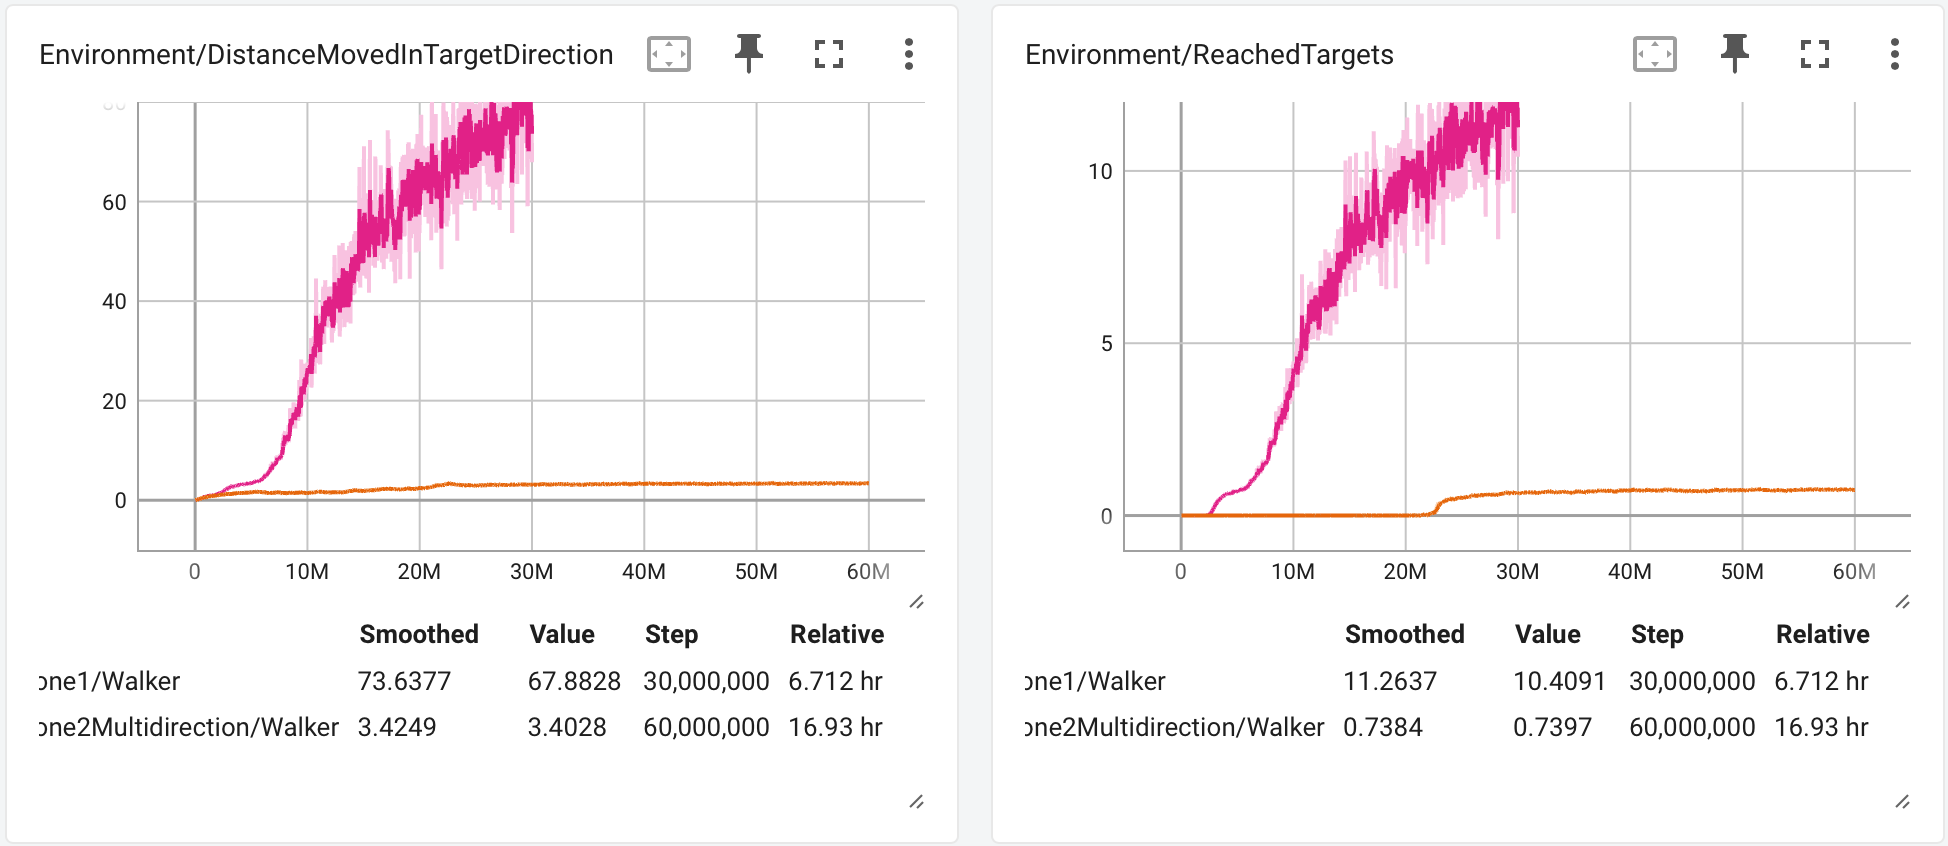
\includegraphics[scale=0.5]{img/versuch8_training.png}
  \caption{Versuch 8 Traininggraphen}
  \label{fig:versuch8_training}
\end{figure}

\begin{figure}[H]
  \centering  
  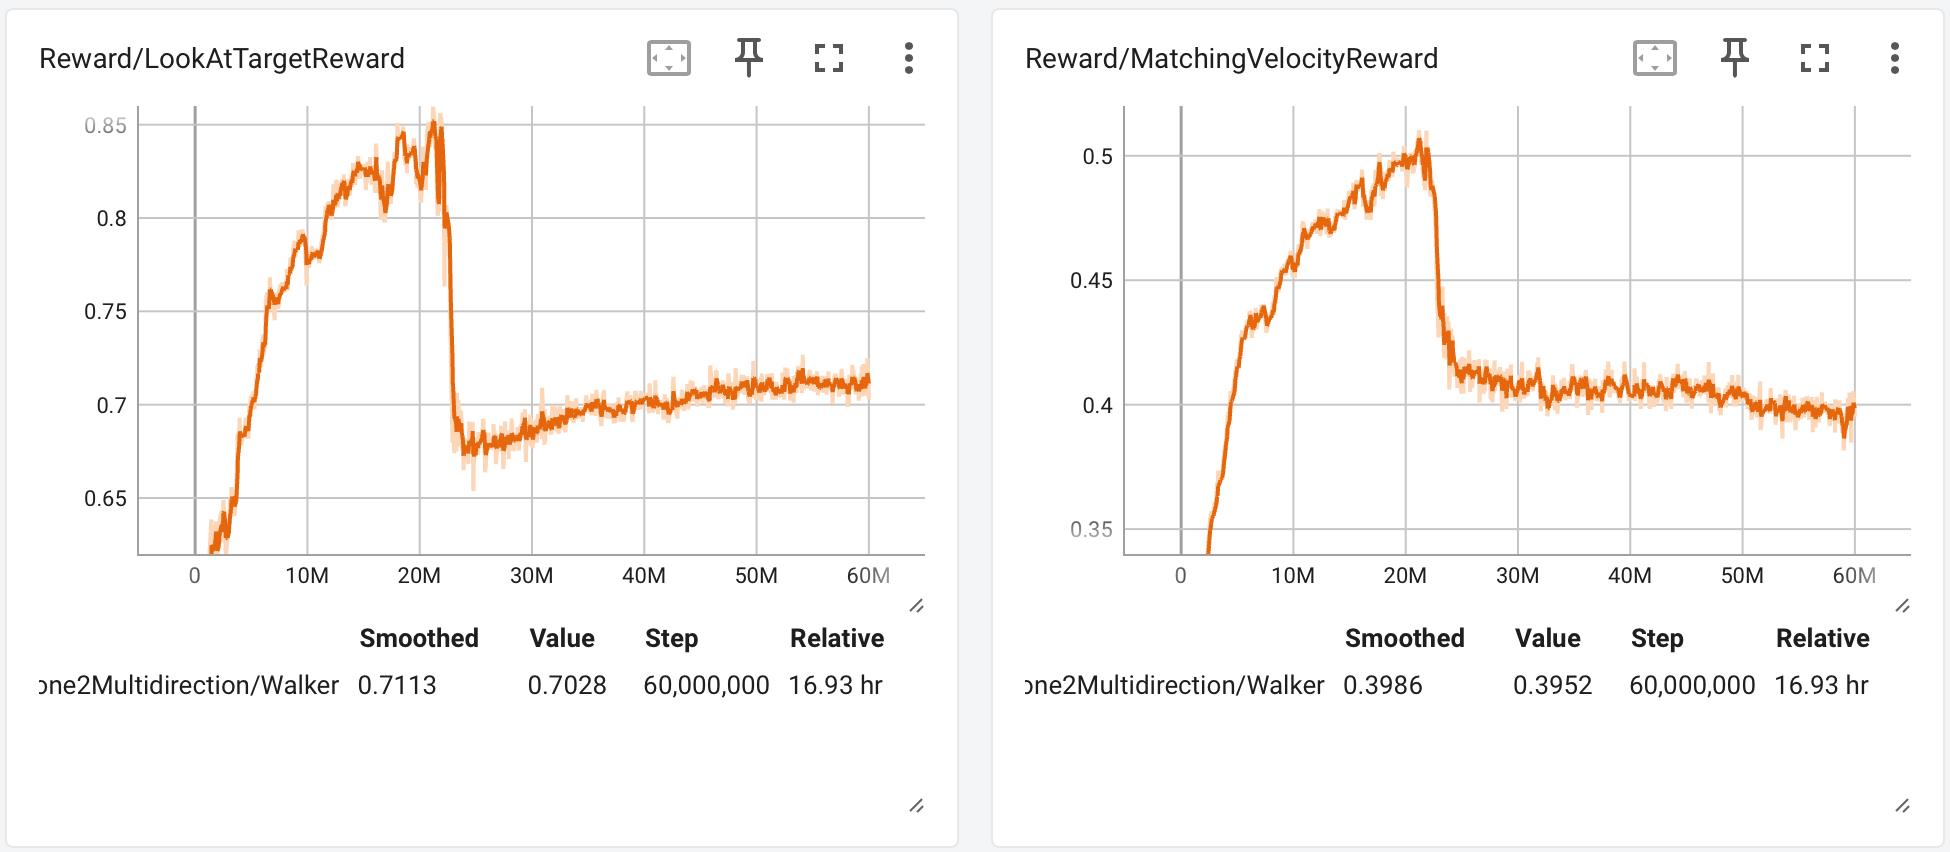
\includegraphics[scale=0.5]{img/versuch8_training_belohnung.png}
  \caption{Versuch 8 Training Belohnungsgraphen}
  \label{fig:versuch8_training_belohnung}
\end{figure}

\subsection{Versuch 9}
Um den Richtungswechsel regelmäßiger zu gestalten, wird getestet wie das Training sich verhält wenn die Richtung beim Start jeder neuen Trainingsepisode zufällig gewählt wird.

\begin{figure}[H]
  \centering  
  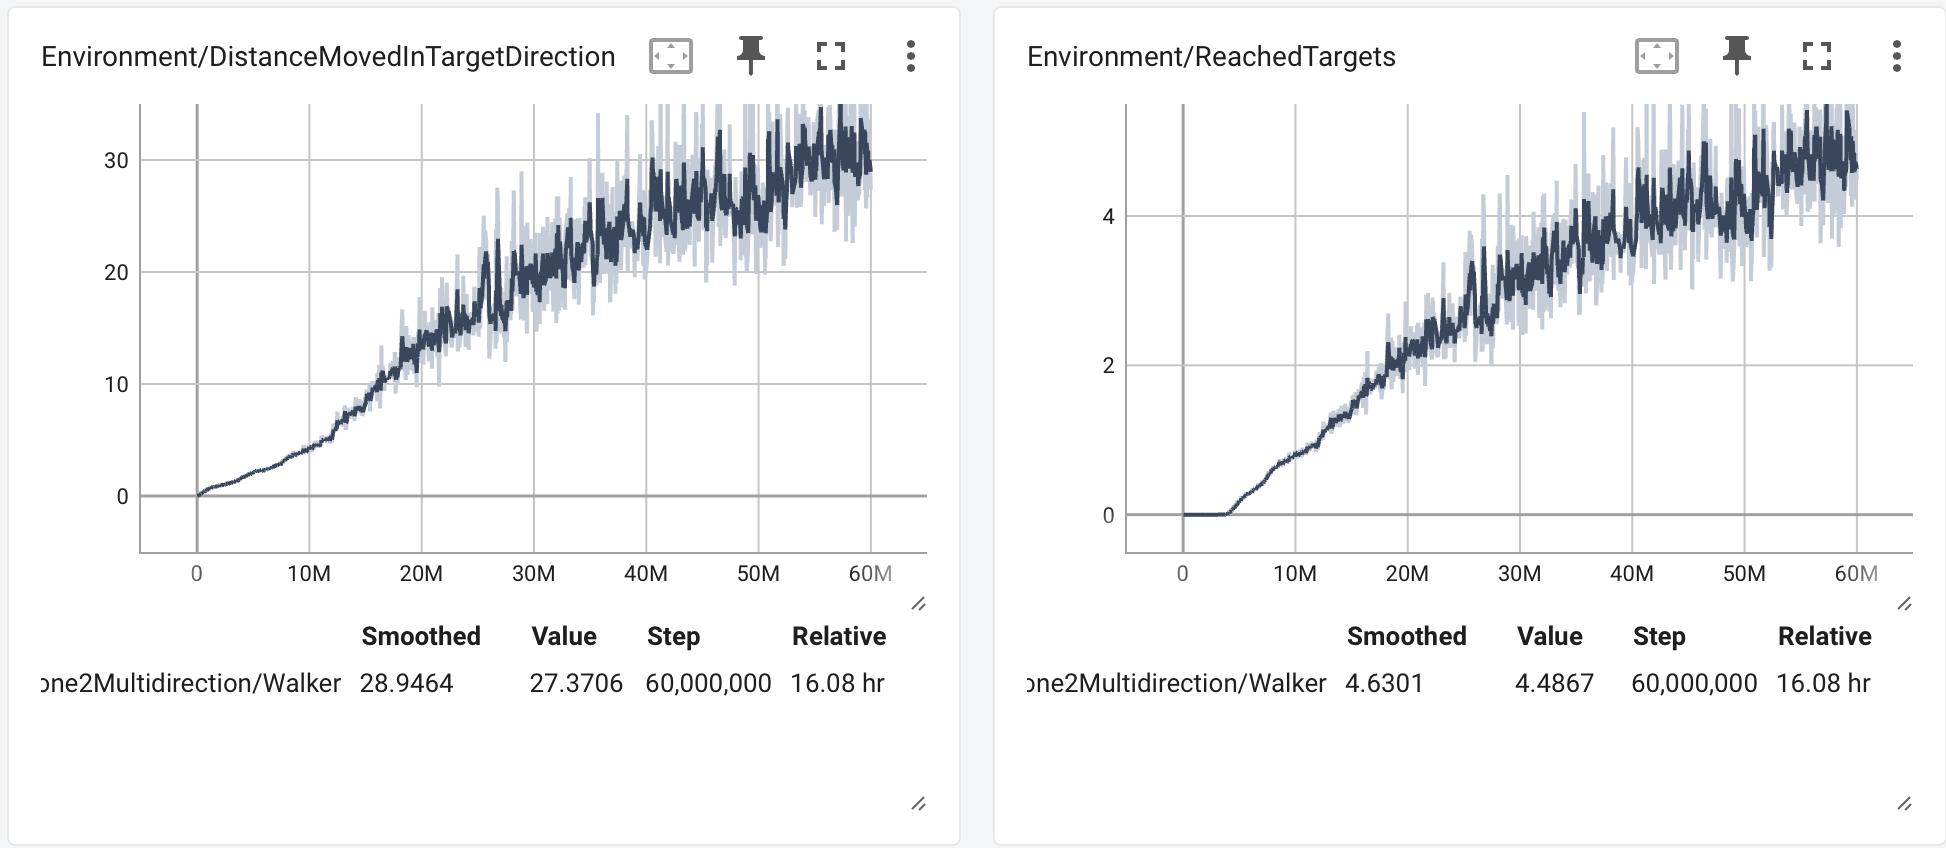
\includegraphics[scale=0.5]{img/versuch9_training.png}
  \caption{Versuch 9 Traininggraphen}
  \label{fig:versuch9_training}
\end{figure}

\begin{figure}[H]
  \centering  
  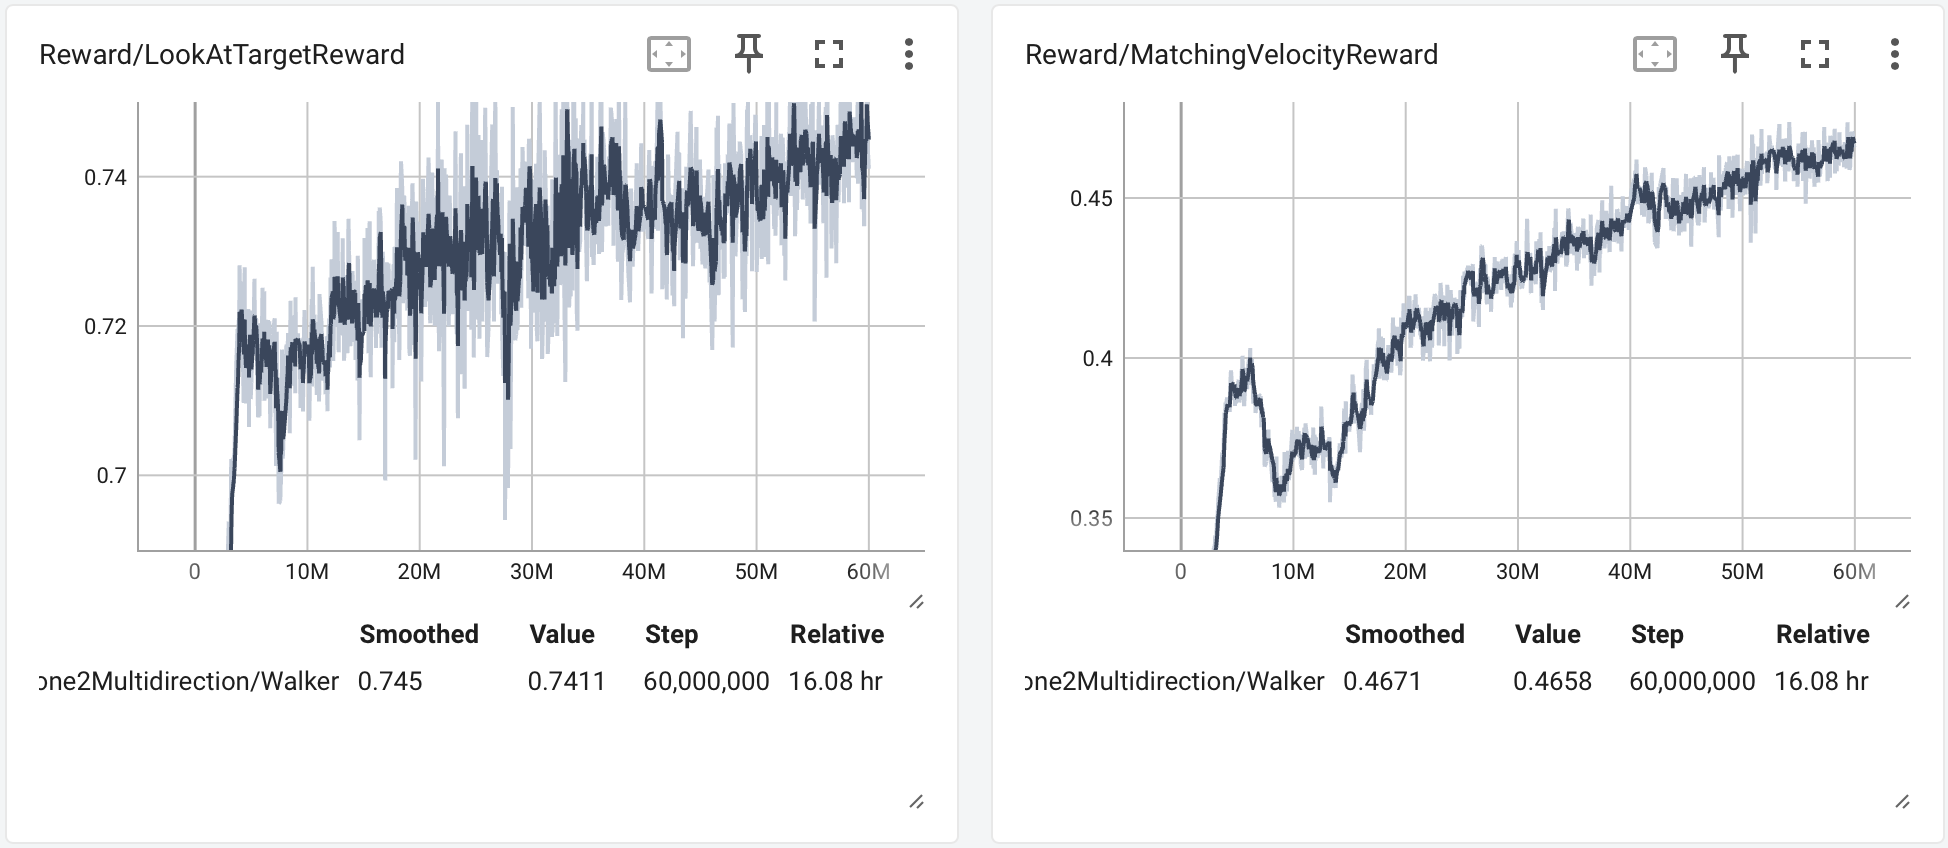
\includegraphics[scale=0.5]{img/versuch9_training_belohnung.png}
  \caption{Versuch 9 Training Belohnungsgraphen}
  \label{fig:versuch9_training_belohnung}
\end{figure}

Das gleichbleiben der Laufbewegung über die komplette Trainingsepisode hat zur folge dass das Training stabiler verläuft siehe Abbildung \ref{fig:versuch8_training}. Der Nachteil ist jedoch das der Läufer keine Bewegungswechsel lernt. Beim steuern des Läufers ist das wechseln zwischen den Laufrichtungen noch immer ein Problem. Dazu kommt das der in diesem training die Blickrichtungs Belohnung geringer ist als bei vorherigen Trainingseinheiten. Der Läufer lernt die seitwärts Bewegungen nicht richtig sondern nimmt einen Verlust in der Belohnung in kauf für die Steigerung der Episodenlänge.
\section{Mixamo Charakter}
Spiele verwenden die unterschiedlichsten Charaktere, nicht nur das Aussehen sondern auch die Komplexität der Körperteile und die Anzahl der Knochen variiert. Um den Charaktercontroller vielseitig einsetzbar zu gestalten wird in diesem Kapitel die Walker Demo Komponenten angepasst um den Einrichtungsprozess zu vereinfachen und unterschiedliche Charakter Körperstrukturen zu erlauben. Es wird der Einrichtungsprozess am Beispiel eines Mixamo 3D Charakter Modells dargestellt. Anschließend werden mit der Mixamo Charakter trainiert und das Ergebnis analysiert. Abschließend werden Verbesserungsansätze für aufgetretene Probleme behandelt.

Der ausgewählte Charakter ist der Y Bot Charakter welcher in Abbildung \ref{fig:y_bot} zu sehen ist. Der Y Bot besteht ausgenommen der Finger und Zehen aus 22 Knochen. Um das Training zu beschleunigen werden für alle Versuche die Zehen als Vorderfuß und die Finger mit dem Handknochen zusammengefaßt.

\begin{figure}[H]
  \centering  
  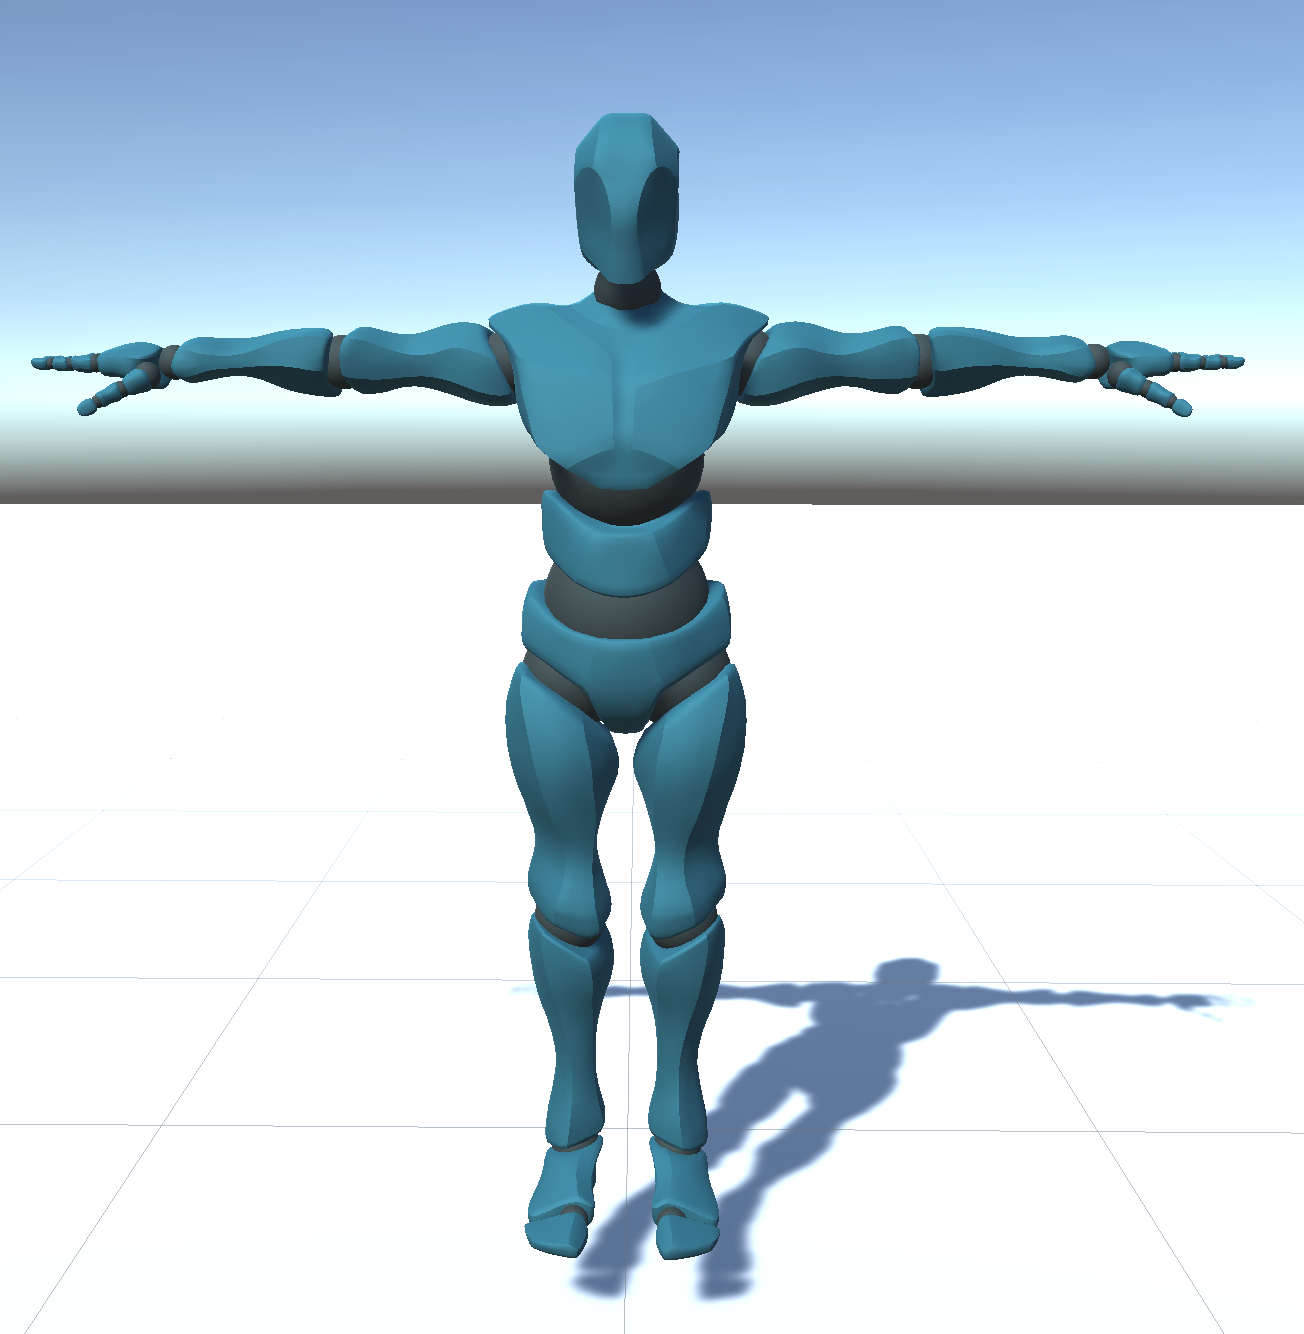
\includegraphics[scale=0.5]{img/y_bot.png}
  \caption{Mixamo Charakter Y Bot}
  \label{fig:y_bot}
\end{figure}

\subsection{Anpassungen}

\subsection{Einrichtung}



Als erstes muss für jedes Körperteile eine passende Kollisionskomponenten ausgewählt und die Größe angepasst werden. Anschließend muss jedes Körperteil eine Festkörperkomponente erhalten. Anschließend müssen die Festkörper- und Gelenkkomponenten hinzugefügt und konfiguriert werden. Die Gewichte der Körperteile wurden im ersten Versuch von der Walker Demo übernommen. Gleichermaßen wurden die Winkellimits für die Gelenke übernommen. Die zusätzlichen Körperteile wurden vereinfacht. Der Oberkörper besteht im Mixamo Modell aus den Schulterknochen sowie dem obersten Wirbel der Wirbelsäule. Die Wirbelsäule besteht im Mixamo Modell aus 2 Wirbeln anstatt dem einen Wirbel des Läufers aus der Demo. Zuletzt sind die Füße noch in Fuß und Vorderfuß aufgeteilt. Bei diesen Änderungen der Körperstruktur wurden die Gewichte und Winkellimits des vereinfachten Körpers auf die komplexeren Körperstrukturen aufgeteilt.

\begin{table}[H]
  \centering
  {\rowcolors{1}{gray!10}{white}
  \begin{tabular}{ |p{3cm}|p{3cm}|p{2cm}|p{4cm}|p{2cm}| }
  \hline
  \textbf{Körpertei}l& \textbf{Verbundenes Körperteil} & \textbf{Gewicht} & \textbf{Winkellimits} & \textbf{Form} \\
  \hline
  Hüfte & - & 15kg & - & Kapsel \\
  \hline
  Wirbel 1 & Hüfte & 6kg & x(-20,20) y(-20,20) z(-15,15) & Kugel \\
  \hline
  Wirbel 2 & Wirbel 1 & 4kg & - & Kugel \\
  \hline
  Wirbel 3 & Wirbel 2 & 3kg & x(-20,20) y(-20,20) z(-15,15) & Kugel \\
  \hline
  Schulter LR & Wirbel 2 & je 2kg& - & Kugel \\
  \hline
  Nacken & Wirbel 3 & 1kg & - & Kugel \\
  \hline
  Kopf & Nacken & 6kg & x(-30,10) y(-20,20) & Kapsel \\
  \hline
  Oberarm LR & Oberkörper & je 4kg & x(-60,120) y(-100,100) & Kapsel \\
  \hline
  Unterarm LR & Oberarm & je 3kg & x(0,160) & Kapsel \\
  \hline
  Hand LR & Unterarm & je 2kg & - & Quader \\
  \hline
  Oberschenkel LR & Hüfte & je 14kg& x(-90,60) y(-40,40) & Kapsel \\
  \hline
  Unterschenkel LR & Oberschenkel & je 7kg &  x(0,120) & Kapsel \\
  \hline
  Fuß LR & Unterschenkel & je 4kg & x(-20,20) y(-20,20) z(-20,20) & Quader \\
  \hline
  Vorderfuß LR & Fuß & je 1kg & - & Quader \\
  \hline
  \end{tabular}}
  \caption{Mixamo Charakter Körperteile}
  \label{table:mixamo_körperteile}
\end{table}

Anschließend kann jedem Körperteil die Körperteilkomponente hinzugefügt werden. Die Körperteilkomponente (Abbildung \ref{fig:körperteil_komponente}) definiert die Körperteile für den Agenten.
\begin{figure}[H]
  \centering  
  \includegraphics[scale=0.5]{img/körperteil_komponente.png}
  \caption{Körperteilkomponente}
  \label{fig:körperteil_komponente}
\end{figure}

\begin{itemize}
  \item Physics Config: legt die Kraft des Gelenks und die maximale rotations Geschwindigkeit der Festkörper fest.
  \item Trigger Touching Ground Event: legt fest ob das Körperteil beim berühren des Bodens ein Event auslöst oder nicht
\end{itemize}

Im letzten Schritt muss noch der Walkeragent hinzugefügt und konfiguriert werden.

\subsection{Versuch 10}
Training vereinfachter Mixamo Charakter. Lernt zu galoppieren.

\begin{figure}[H]
  \centering
  \begin{tabular}{cccc}
    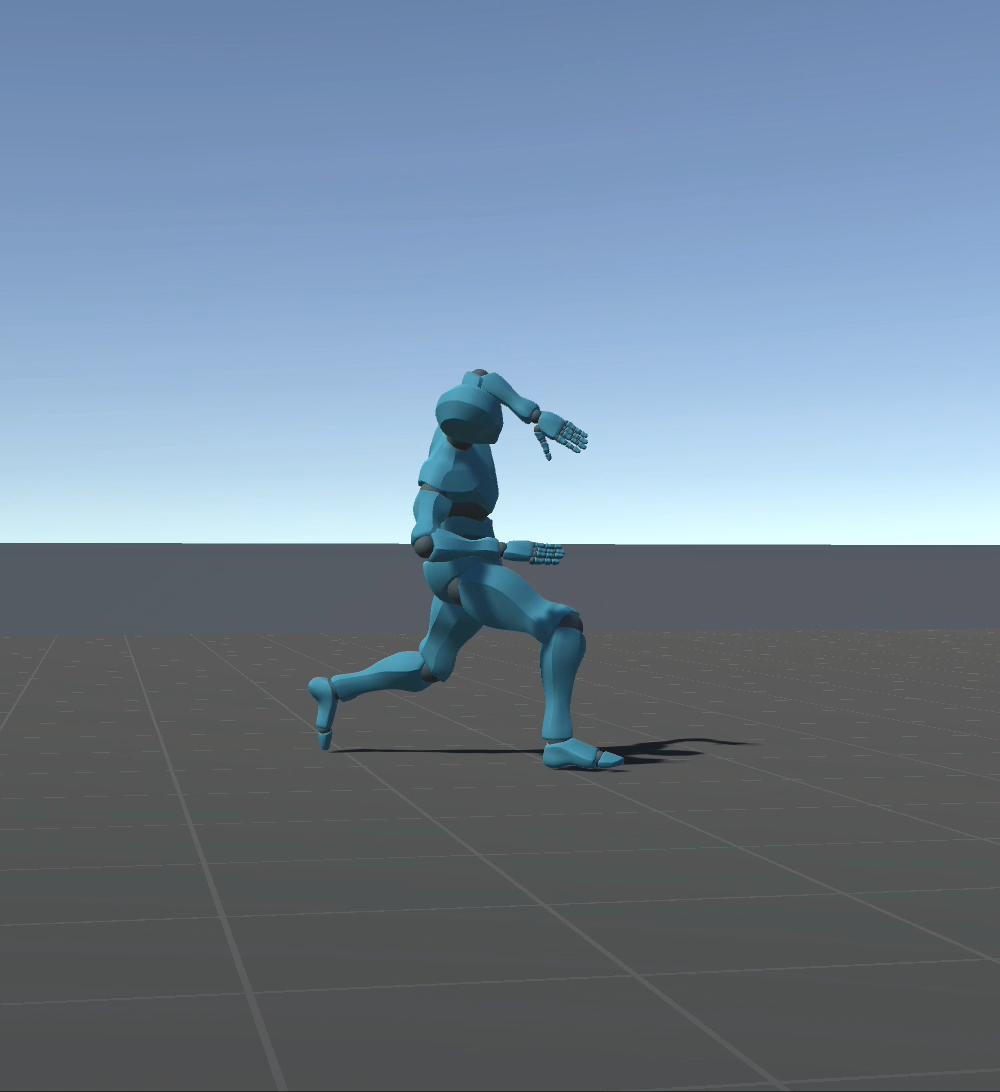
\includegraphics[width=0.2\textwidth]{img/mixamo_galoppieren1.png} & 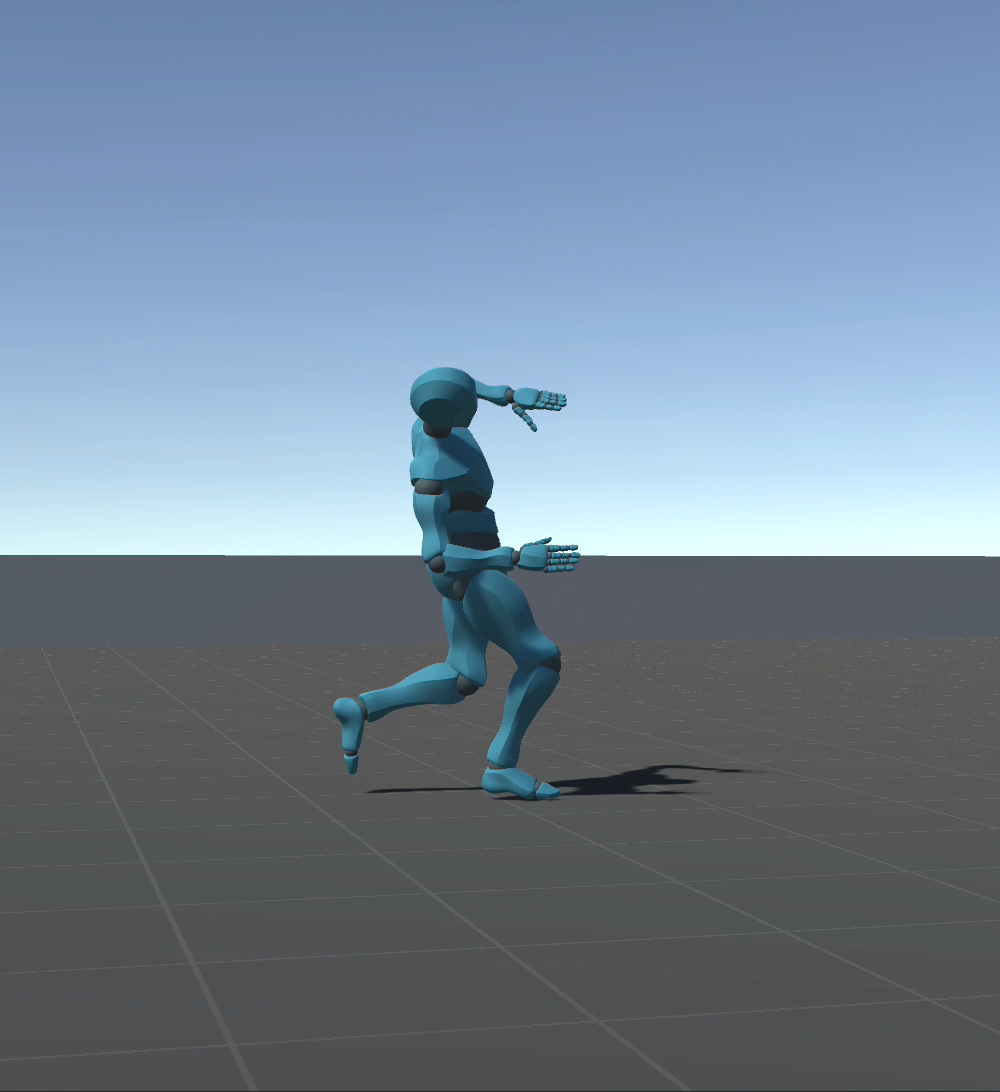
\includegraphics[width=0.2\textwidth]{img/mixamo_galoppieren2.png} & 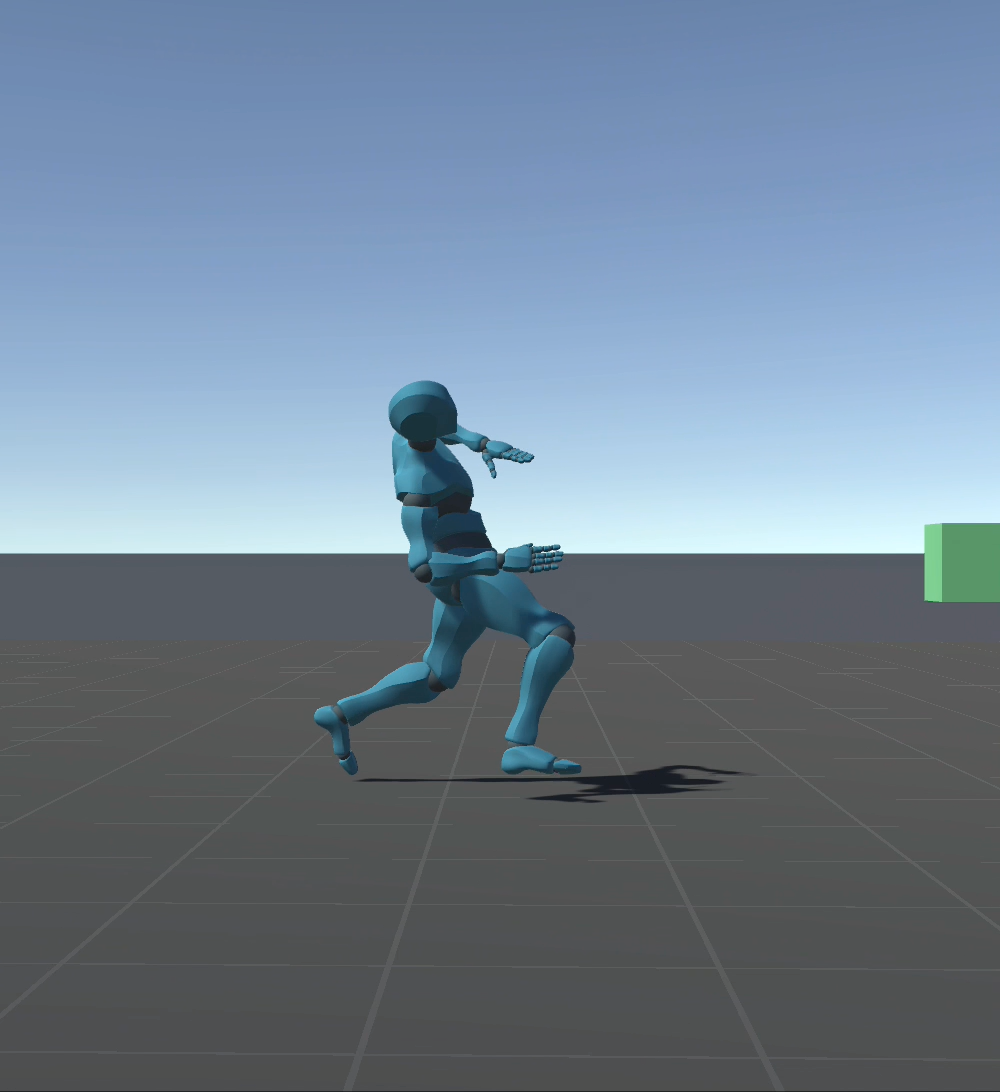
\includegraphics[width=0.2\textwidth]{img/mixamo_galoppieren3.png} & 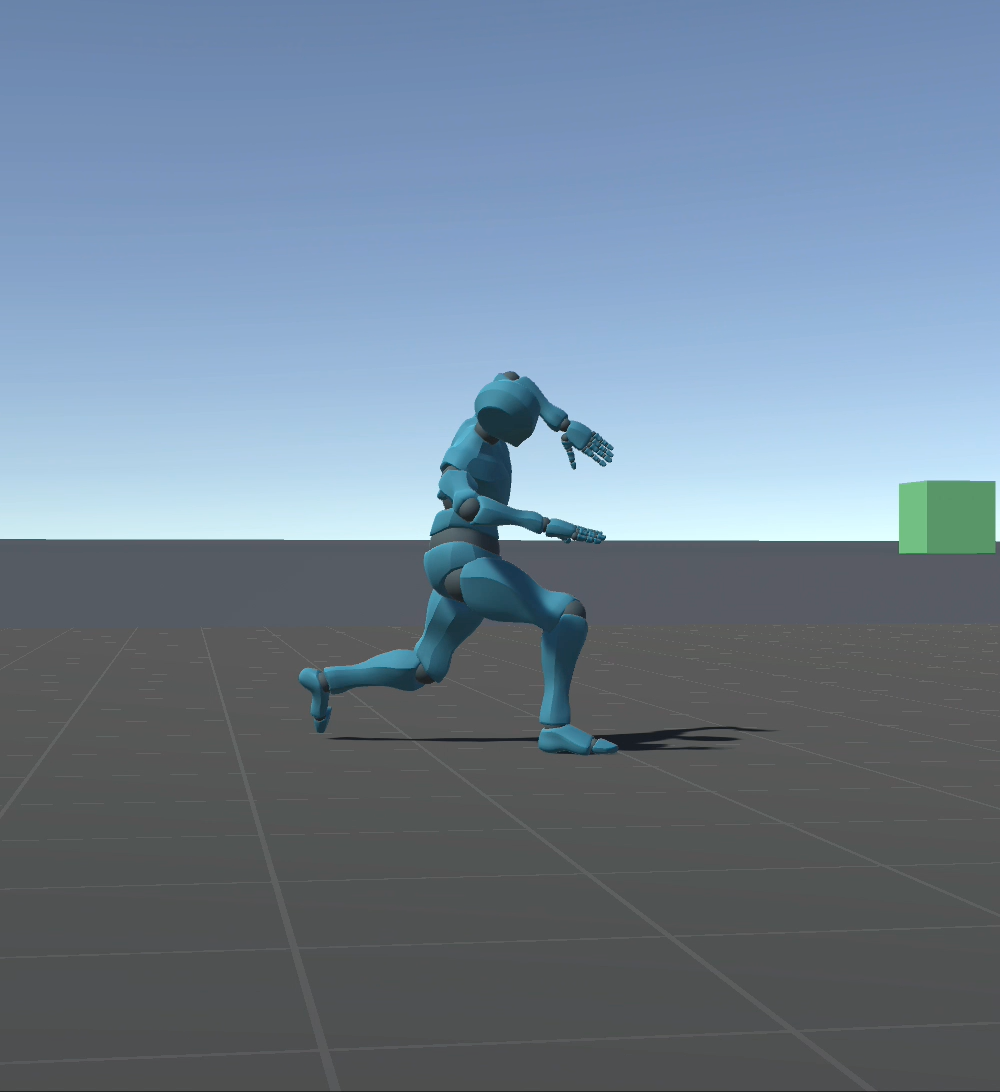
\includegraphics[width=0.2\textwidth]{img/mixamo_galoppieren4.png} \\
  \end{tabular}
  \caption{Mixamo Versuch 10 Gangbild}
  \label{fig:mixamo_versuch10_gangbild}
\end{figure}

\subsection{Versuch 11}
Hinzufügen von Beinwechsel Belohnung. Lernt mit periodischem Beinwechsel zu laufen.

\begin{figure}[H]
  \centering
  \begin{tabular}{ccc}
    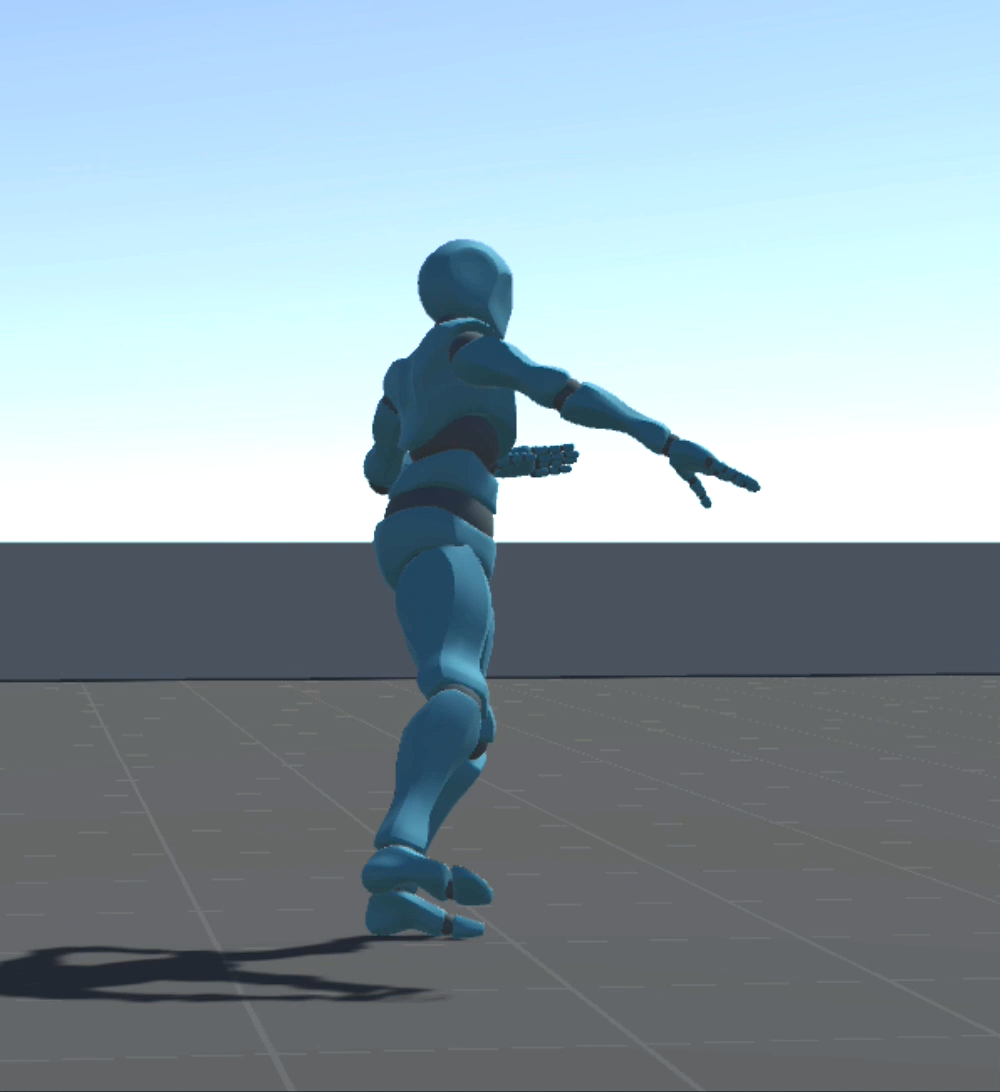
\includegraphics[width=0.27\textwidth]{img/mixamo_laufen1.png} & 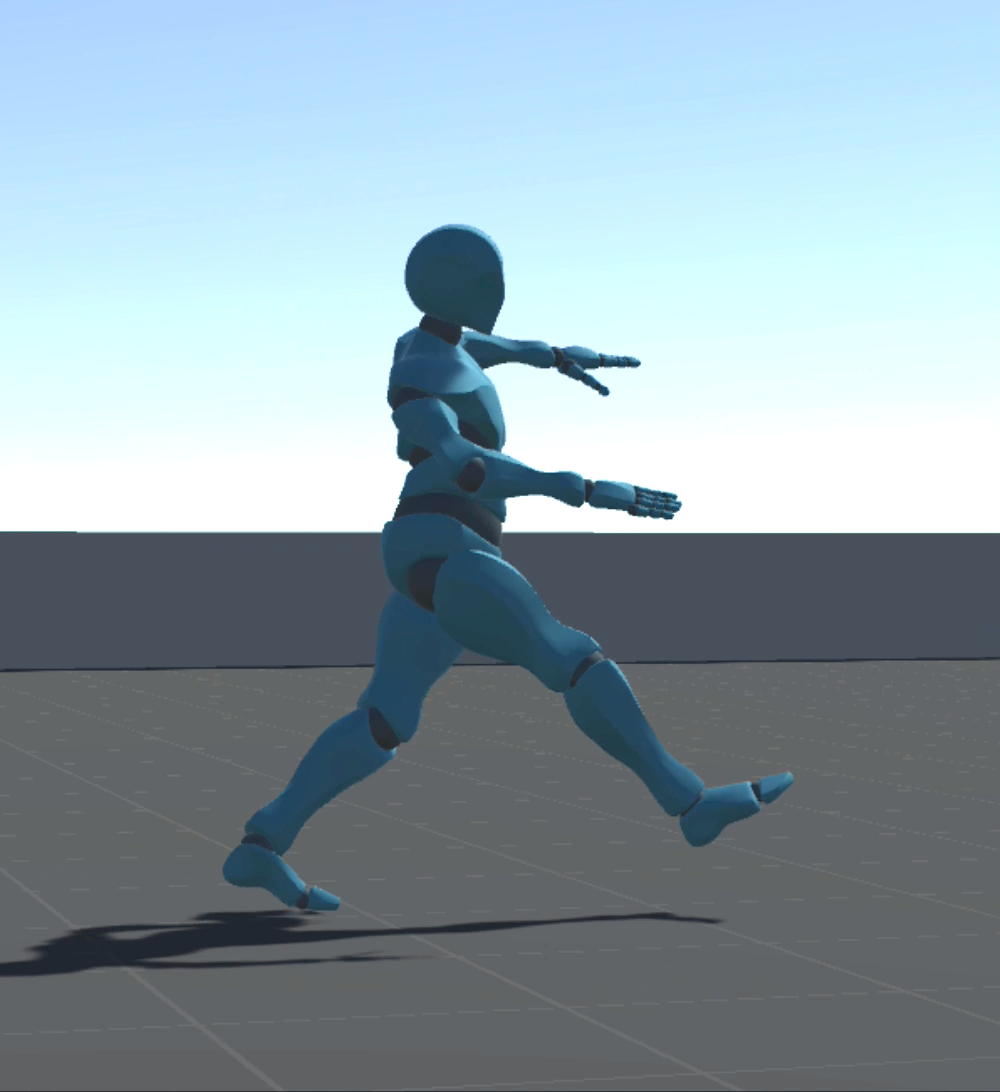
\includegraphics[width=0.27\textwidth]{img/mixamo_laufen2.png}  & 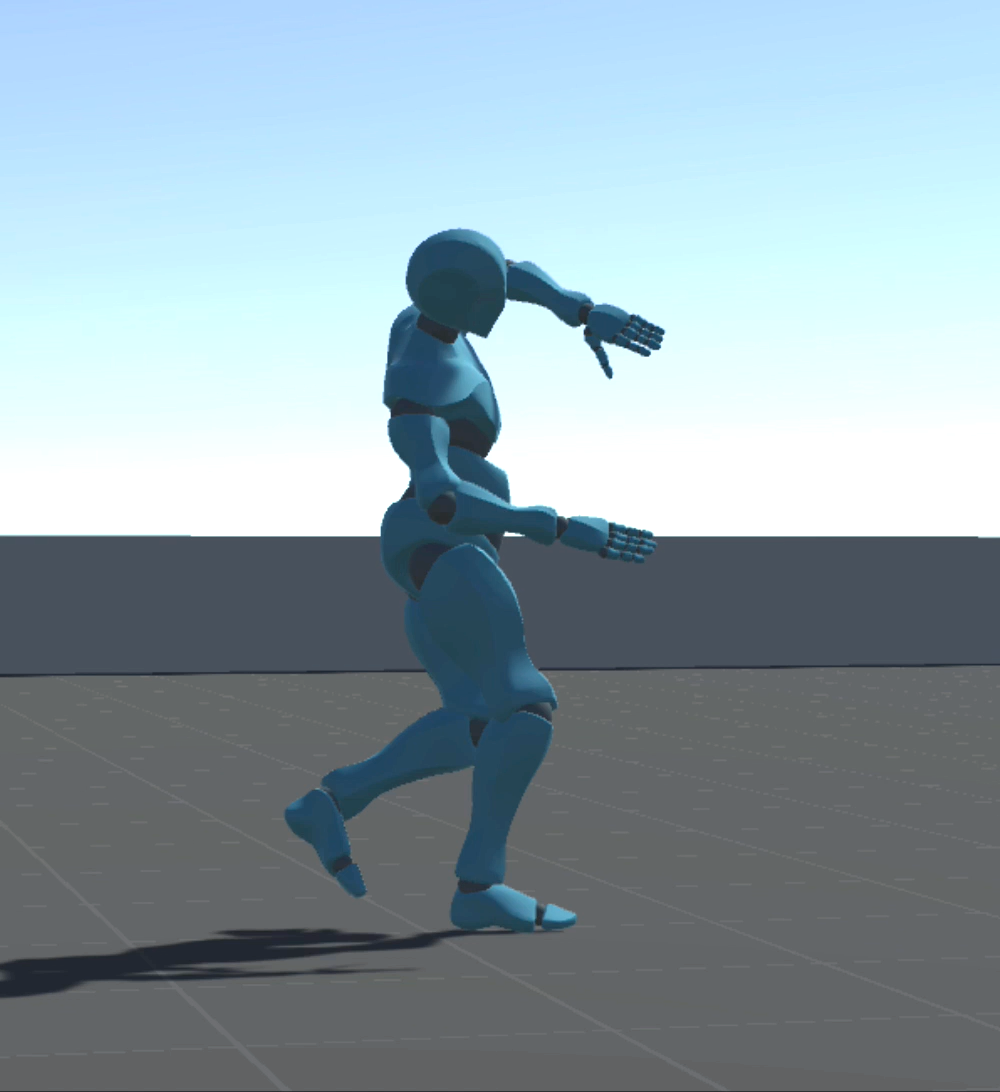
\includegraphics[width=0.27\textwidth]{img/mixamo_laufen3.png} \\
    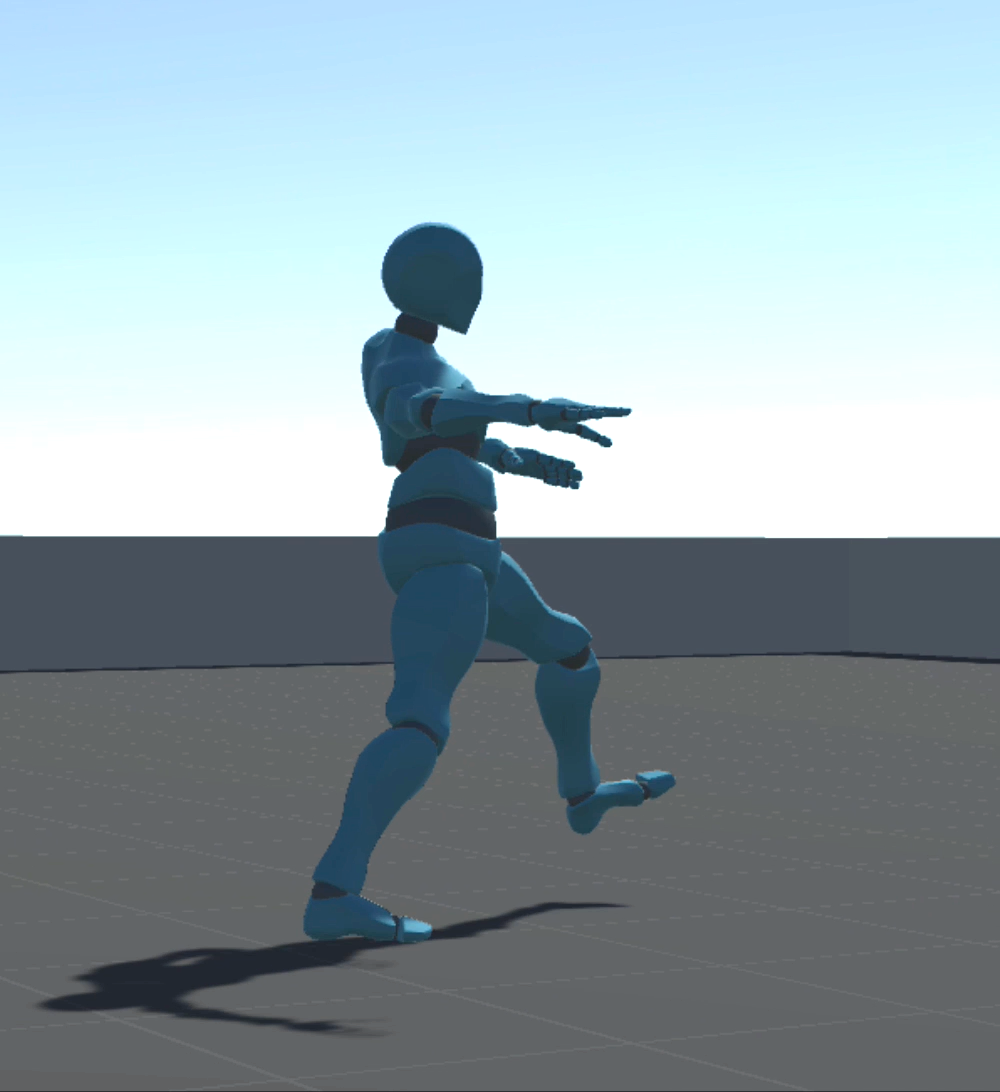
\includegraphics[width=0.27\textwidth]{img/mixamo_laufen4.png}  & 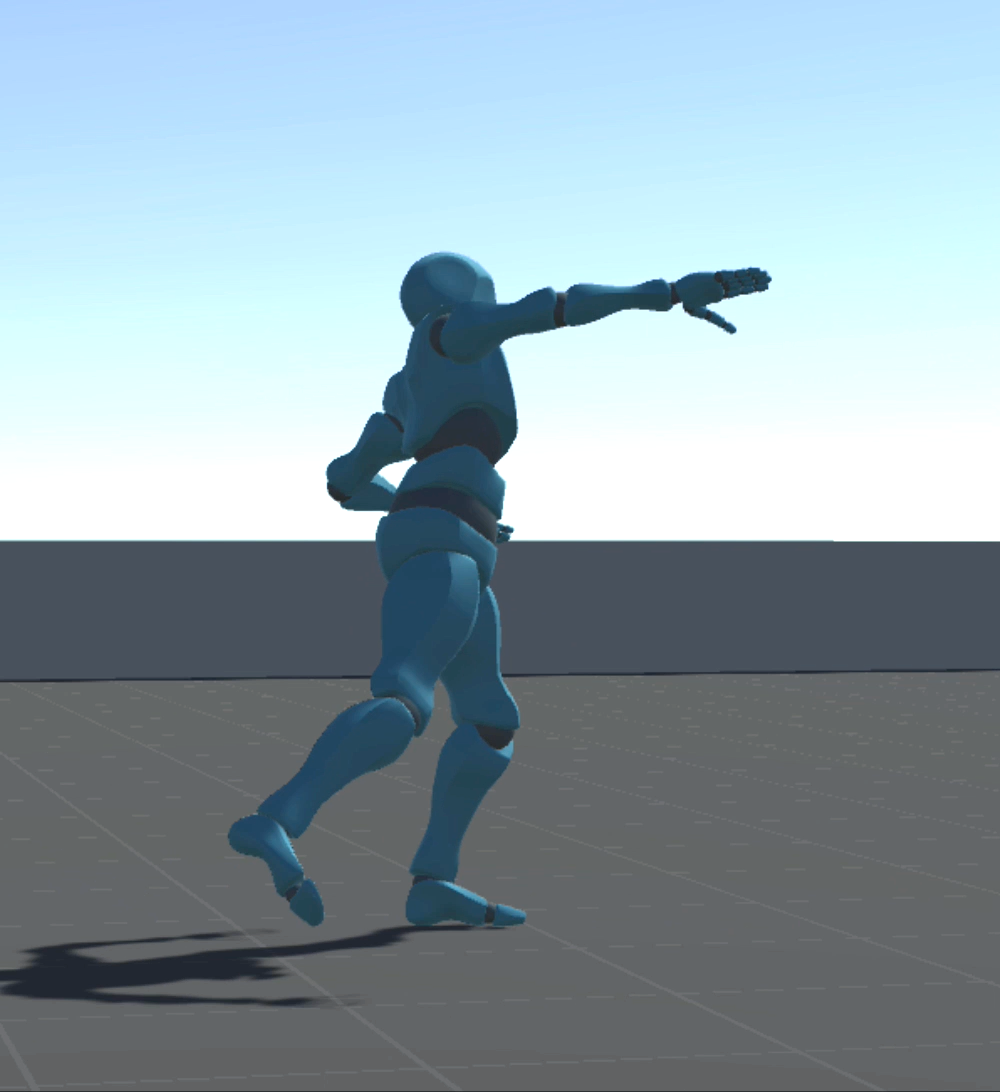
\includegraphics[width=0.27\textwidth]{img/mixamo_laufen5.png}  & 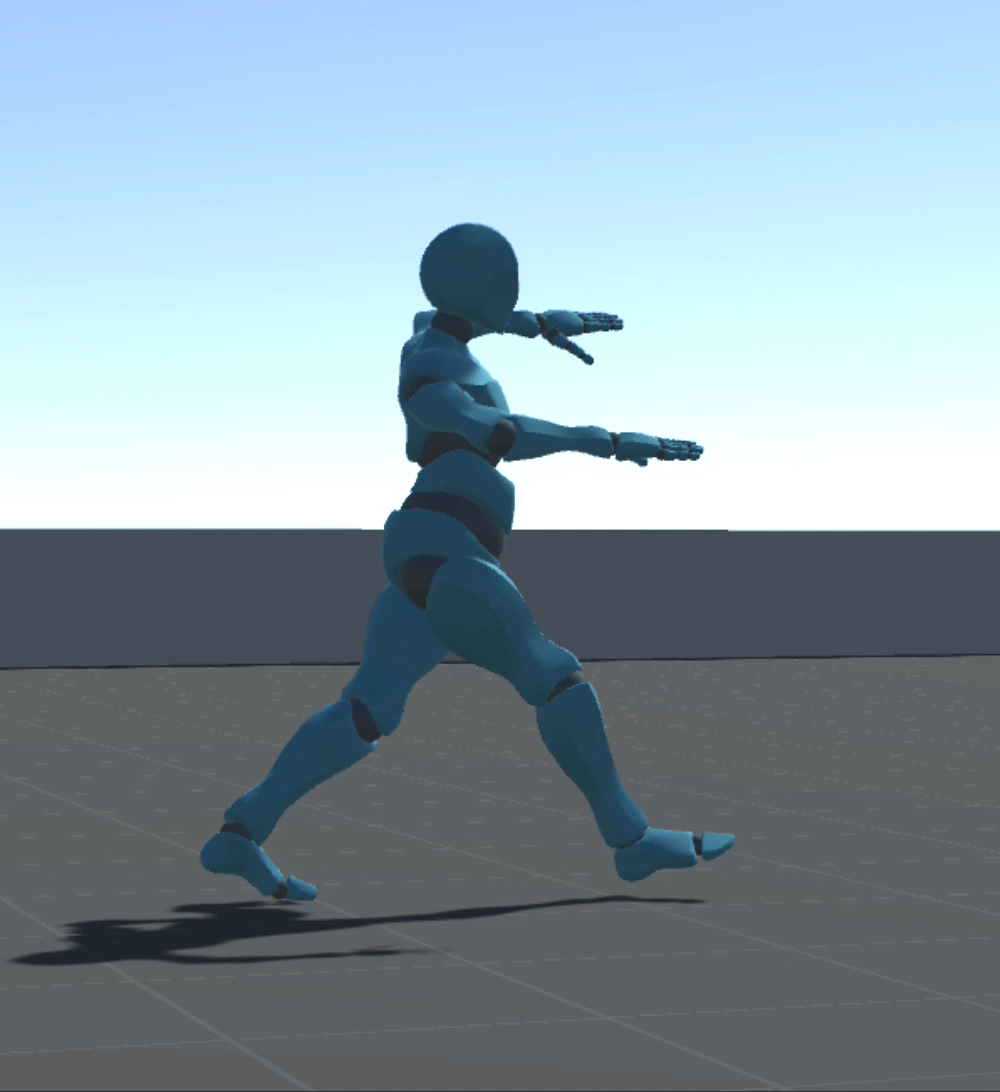
\includegraphics[width=0.27\textwidth]{img/mixamo_laufen6.png} \\
  \end{tabular}
  \caption{Mixamo Versuch 11 Gangbild}
  \label{fig:mixamo_versuch11_gangbild}
\end{figure}

\subsection{Versuch 12}
Energiespar Belohnung um Gangbild natürlicher zu machen. Gangbild wird natürlicher aber Arme sind noch sehr starr und nah am Körper.

\begin{figure}[H]
  \centering
  \begin{tabular}{ccc}
    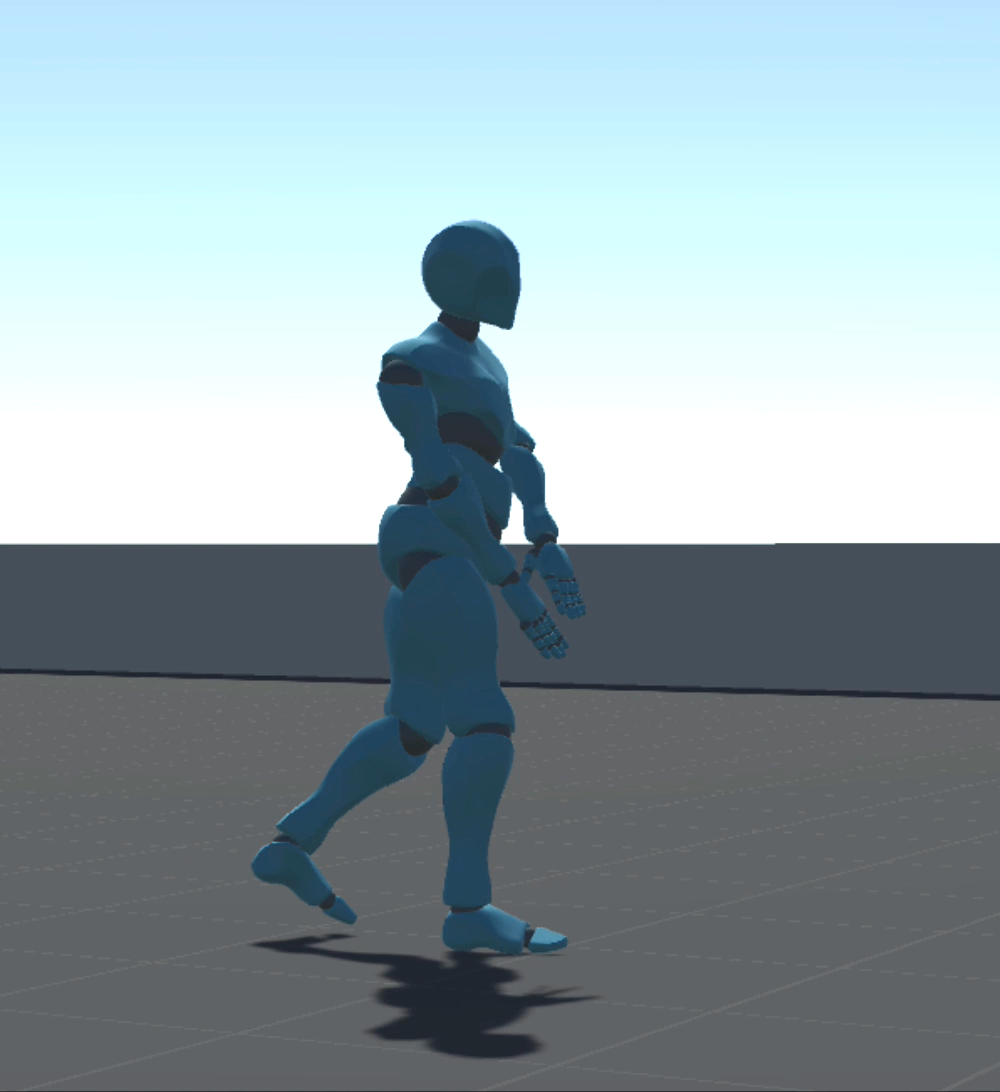
\includegraphics[width=0.27\textwidth]{img/mixamo_laufen_energiespar1.png} & 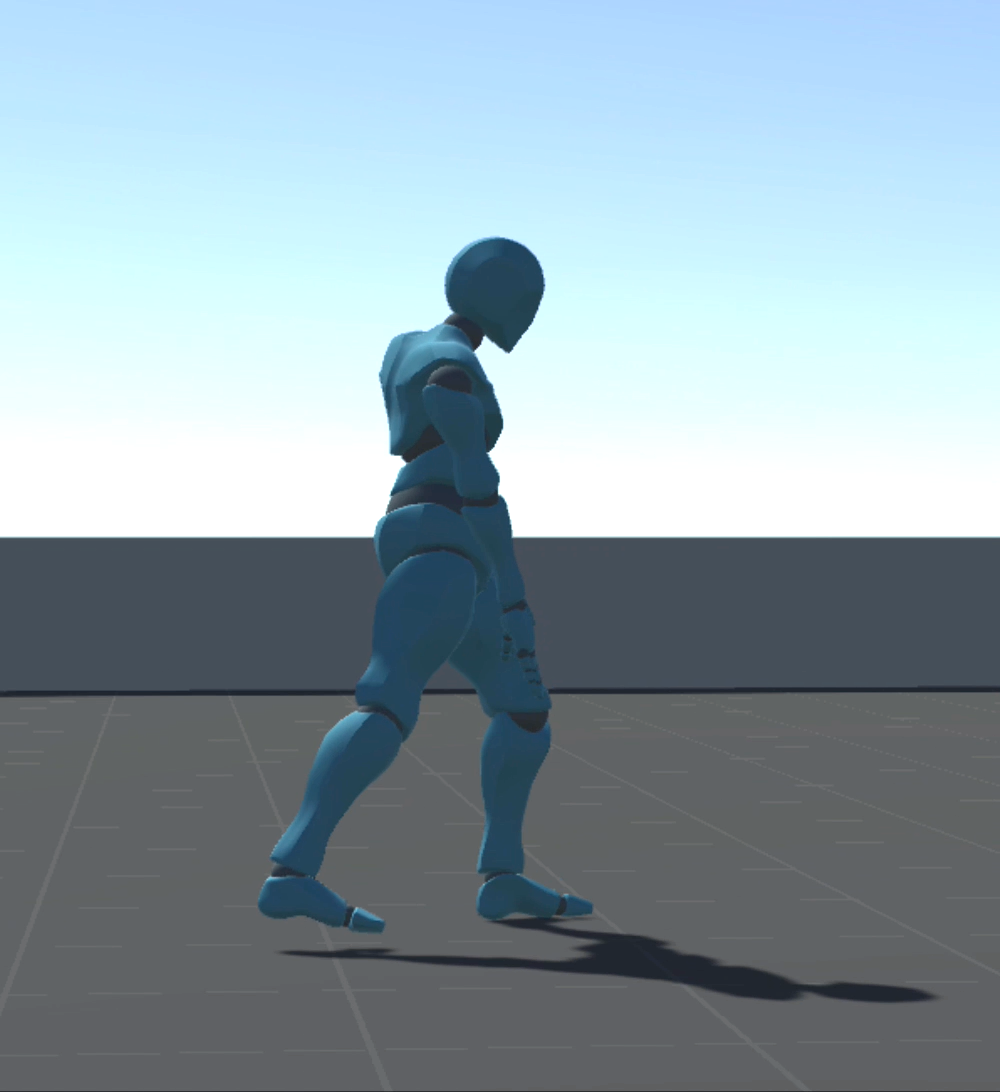
\includegraphics[width=0.27\textwidth]{img/mixamo_laufen_energiespar2.png}  & 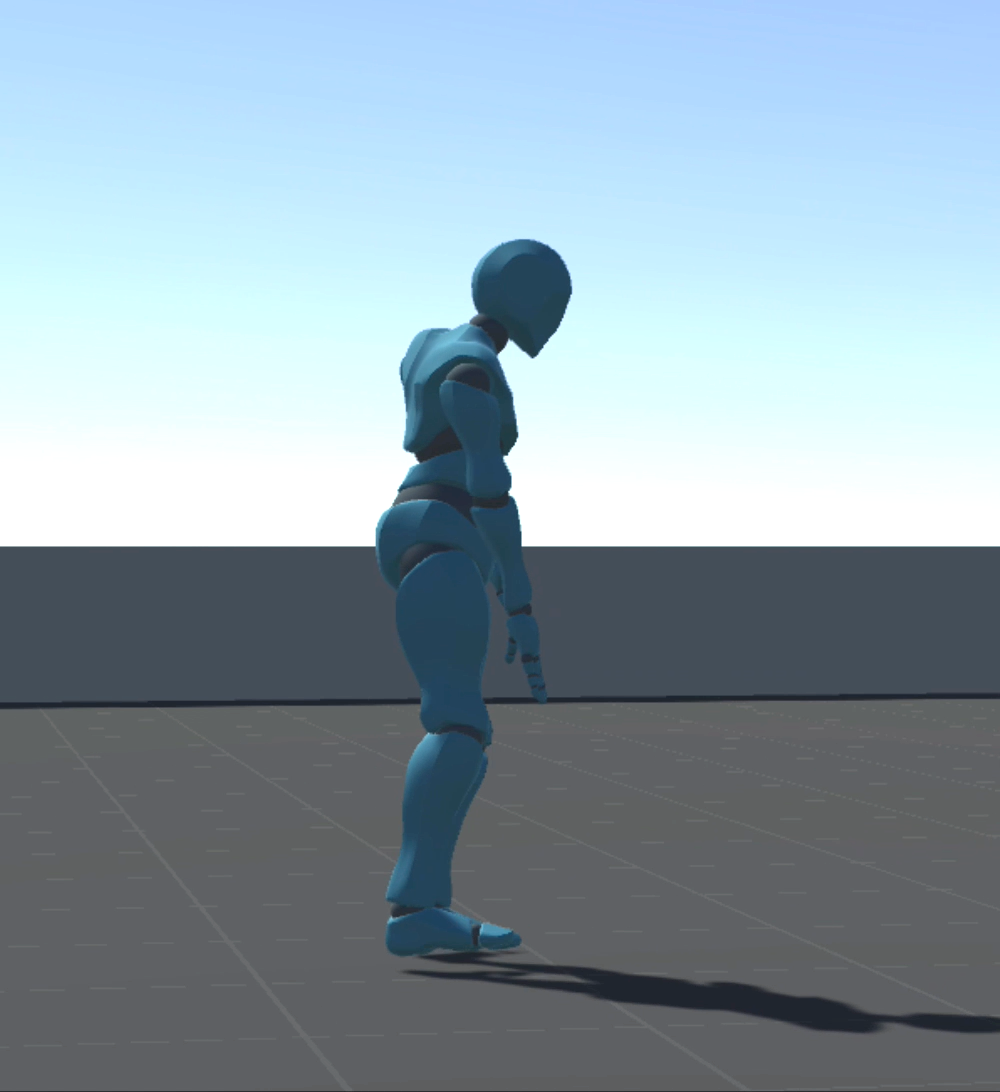
\includegraphics[width=0.27\textwidth]{img/mixamo_laufen_energiespar3.png} \\
    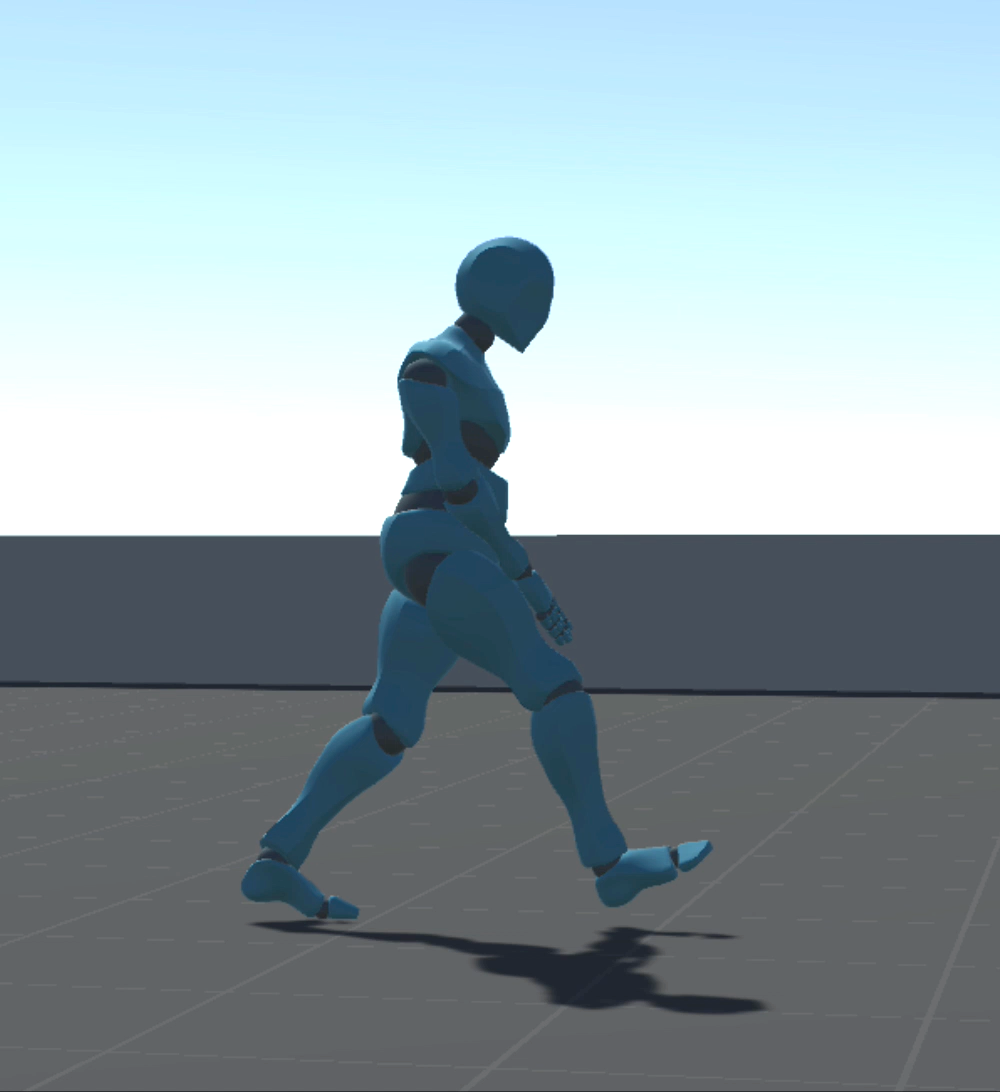
\includegraphics[width=0.27\textwidth]{img/mixamo_laufen_energiespar4.png}  & 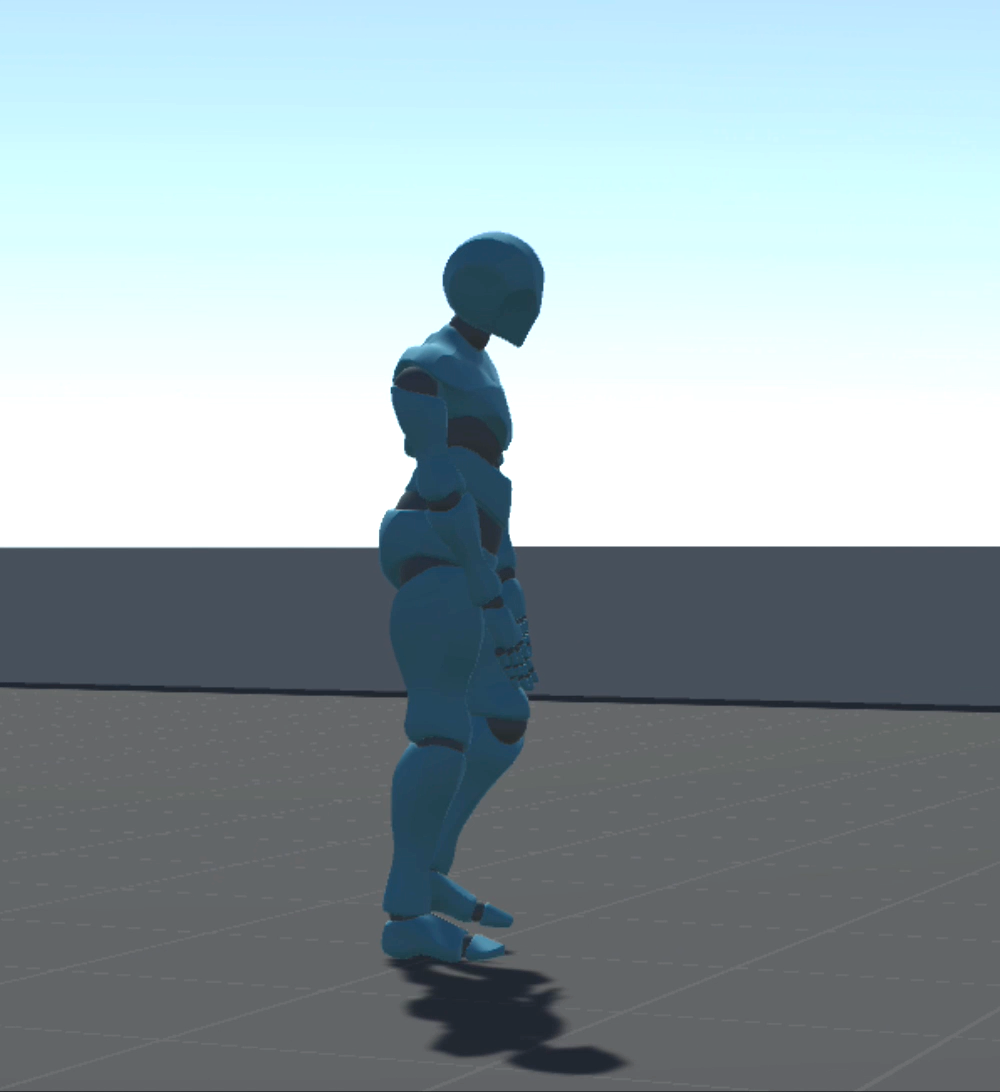
\includegraphics[width=0.27\textwidth]{img/mixamo_laufen_energiespar5.png}  & 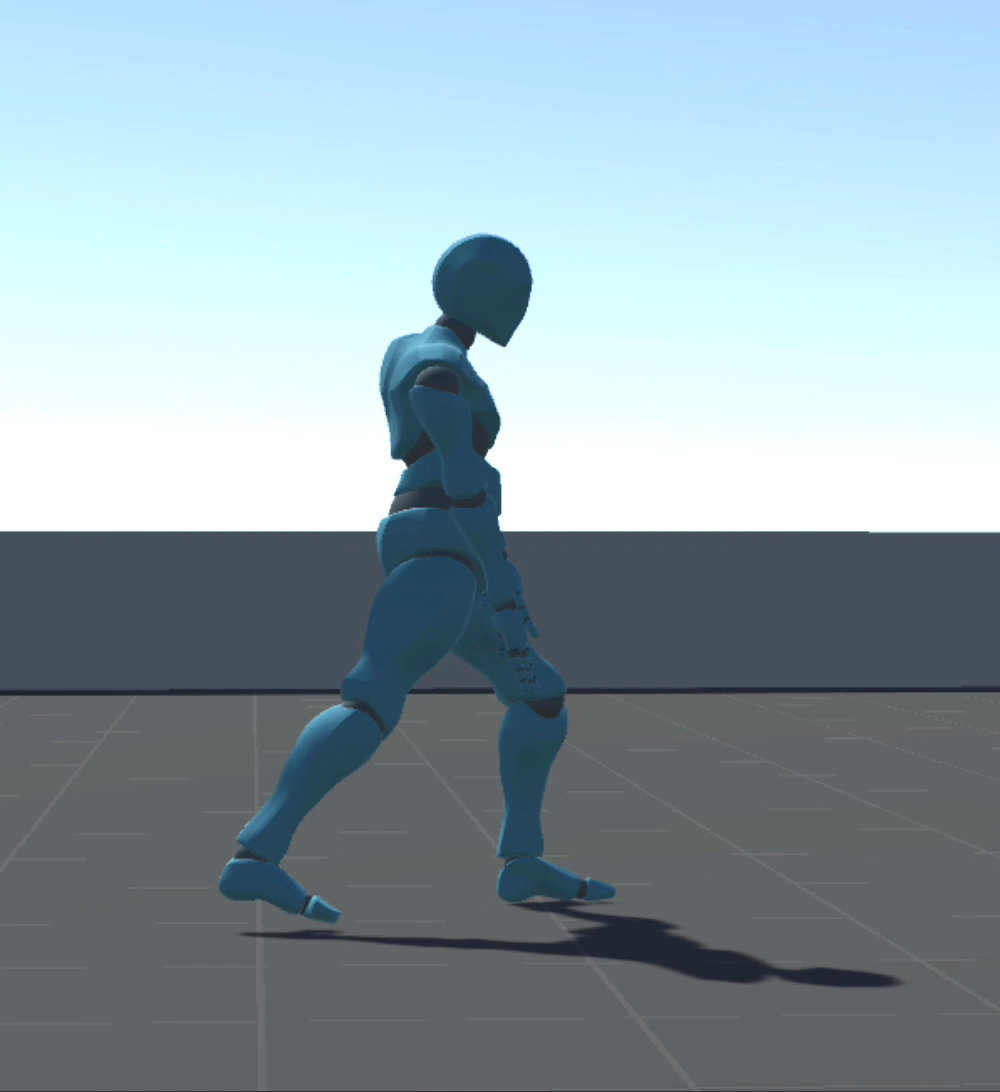
\includegraphics[width=0.27\textwidth]{img/mixamo_laufen_energiespar6.png} \\
  \end{tabular}
  \caption{Mixamo Versuch 12 Gangbild}
  \label{fig:mixamo_versuch12_gangbild}
\end{figure}

-Beinwechsel Belohnung um galoppieren zu vermeiden -> funktioniert
-Leistungsminimierung Belohnung um laufverhalten natürlicher zu machen -> funktioniert nur arme sind sehr nah und starr am Körper
-
\section{Gangbild Anpassungen}
Das natürlich erlernte Gangbild eines gesunden Menschen ist sehr komplex. Im folgenden Kapitel wird das Gangbild des Mixamo Charakters basierend auf den Gangphasen der menschlichen Fortbewegung analysiert und angepasst. Diese Gangphasen umfassen verschiedene Stadien der Fortbewegung, wie das Abstoßen, das Schwingen des Beins und den Fersenauftritt, die zusammen ein fließendes und ausgewogenes Gehen ermöglichen. Wie bereits in der Analyse der Walker Demo erwähnt, ist das Gangbild des Walker Demo Läufers menschenähnlich und für die vereinfachte Darstellung des Charakters durchaus ausreichend. Die gesteigerte Komplexität des 3D-Modells beim Mixamo Charakter führt bei der Wahrnehmung zu einem gesteigerten Realismus. Der Mixamo Charakter lernt zudem eher ein Galoppieren als das Laufen, welches der Walker Demo Läufer nach dem Training aufweist. Durch den gesteigerten Realismus und die Verschlechterung des Gangbilds wird im folgenden Kapitel untersucht, wie zusätzliche Belohnungen das erlernte Gangbild beeinflussen können. Dabei werden gezielt Belohnungen eingeführt, die darauf abzielen, das Gesamterscheinungsbild der Fortbewegung zu verbessern. Der Code zu den in folgenden Abschnitten entwickelten Belohnungen ist in \ref{code:gehbewegung_belohnung} zu finden.

\subsection{Beinwechsel}
Das menschliche Gangbild besteht aus sich wiederholenden Phasen, die abwechselnd bei beiden Beinen durchlaufen werden. Um den Läufer dazu zu motivieren, in einem regelmäßigen Intervall das vorangehende Bein zu wechseln, wird ein Timer eingeführt, der von 0 startet, sobald das vorderste Bein in Zielrichtung gewechselt wurde. Ausgehend von der verstrichenen Zeit seit dem letzten Wechsel erhält der Läufer dann eine Strafe. Wie in Abbildung \ref{fig:plot_beinwechsel} zu sehen ist, bleibt die Bestrafung bis 1,2 Sekunden bei 0. Bleibt ein Bein länger als 1,2 Sekunden vorne, steigt die Bestrafung linear an, bis sie bei 5,2 Sekunden das Maximum von -1 erreicht. Initial wurde ein Schwellenwert für die Bestrafung von 2 Sekunden von einem ähnlichen Projekt aus dem Youtube Video \grqq{}AI Learns to Walk (deep reinforcement learning)\grqq{} übernommen.\cite{aiwarehouse} Nach dem Training war jedoch deutlich zu sehen, dass eine Beinwechselperiode von 2 Sekunden zu lang ist. Durch eigene Experimente des Verfassers wurde eine durchschnittliche Beinwechselzeit von 1,2 Sekunden ermittelt. Für die Bestimmung dieses Wertes wurden Videoaufnahmen des Gehens erstellt, anhand derer anschließend die Dauer eines Beinwechsels festgelegt werden konnte.

\begin{figure}[H]
  \centering
  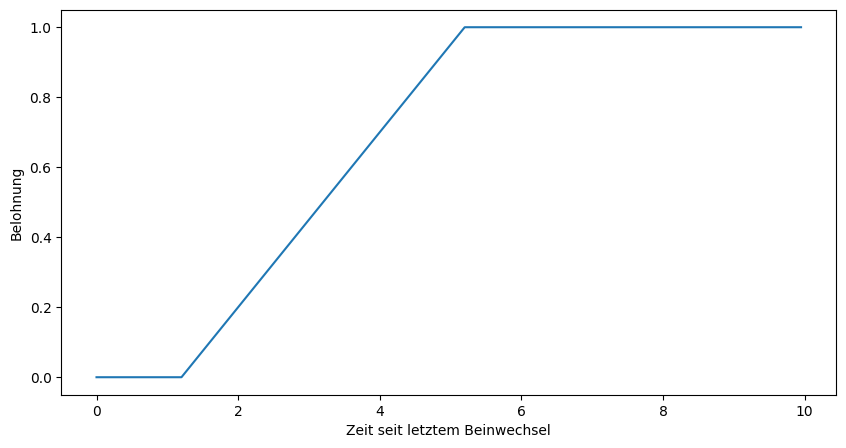
\includegraphics[width=0.85\textwidth]{img/plot_beinwechsel} 
  \caption{Beinwechselbelohnung}
  \label{fig:plot_beinwechsel}
\end{figure}

Das Einführen dieser Bestrafung hat beim Training erfolgreich dazu geführt, dass der Läufer in regelmäßigen Abständen das Standbein wechselt (siehe Abbildung \ref{fig:mixamo_versuch11_gangbild}). Diese Anpassung führte zu einer spürbaren Verbesserung der Bewegungsdynamik des Läufers, insbesondere in Bezug auf die Regelmäßigkeit der Schritte.

\begin{figure}[H]
  \centering
  \begin{tabular}{ccc}
    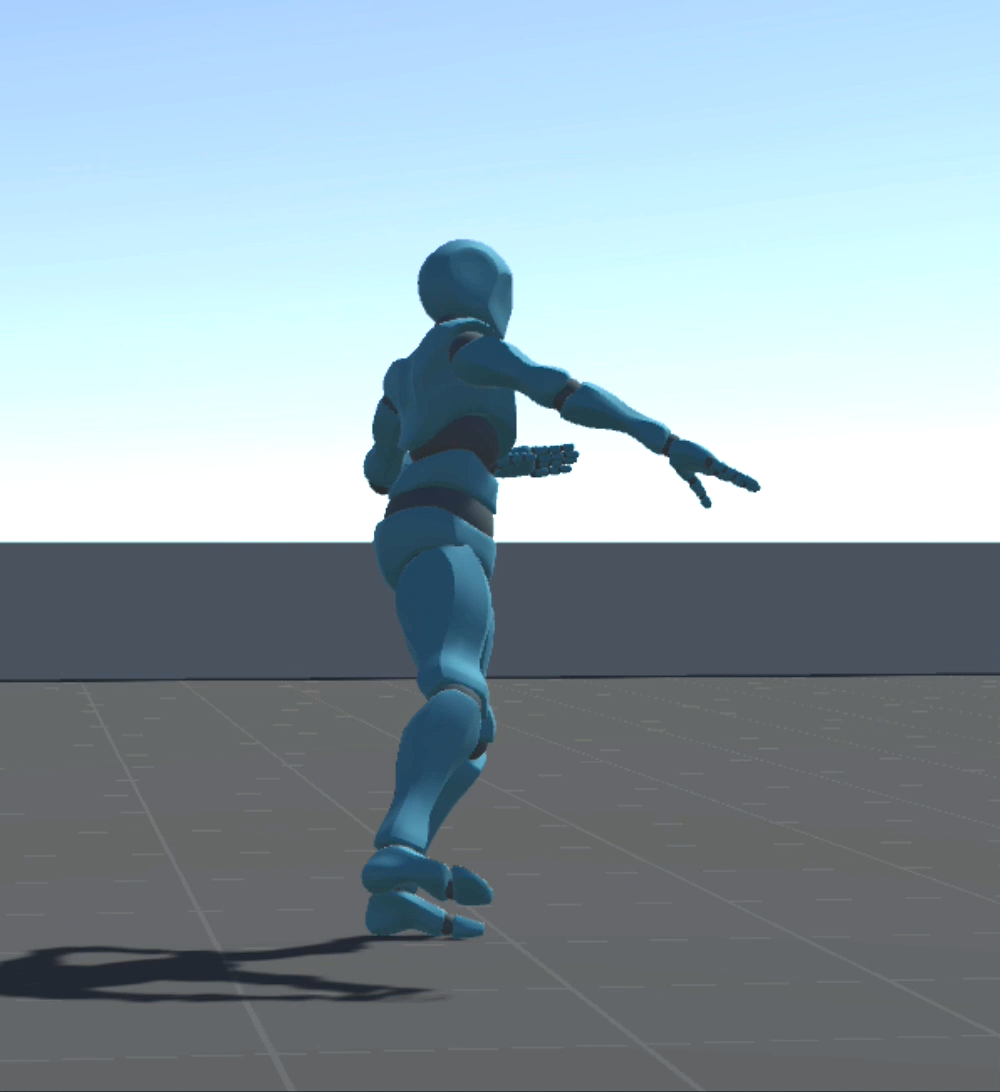
\includegraphics[width=0.27\textwidth]{img/charakter_mixamo_laufen1} & 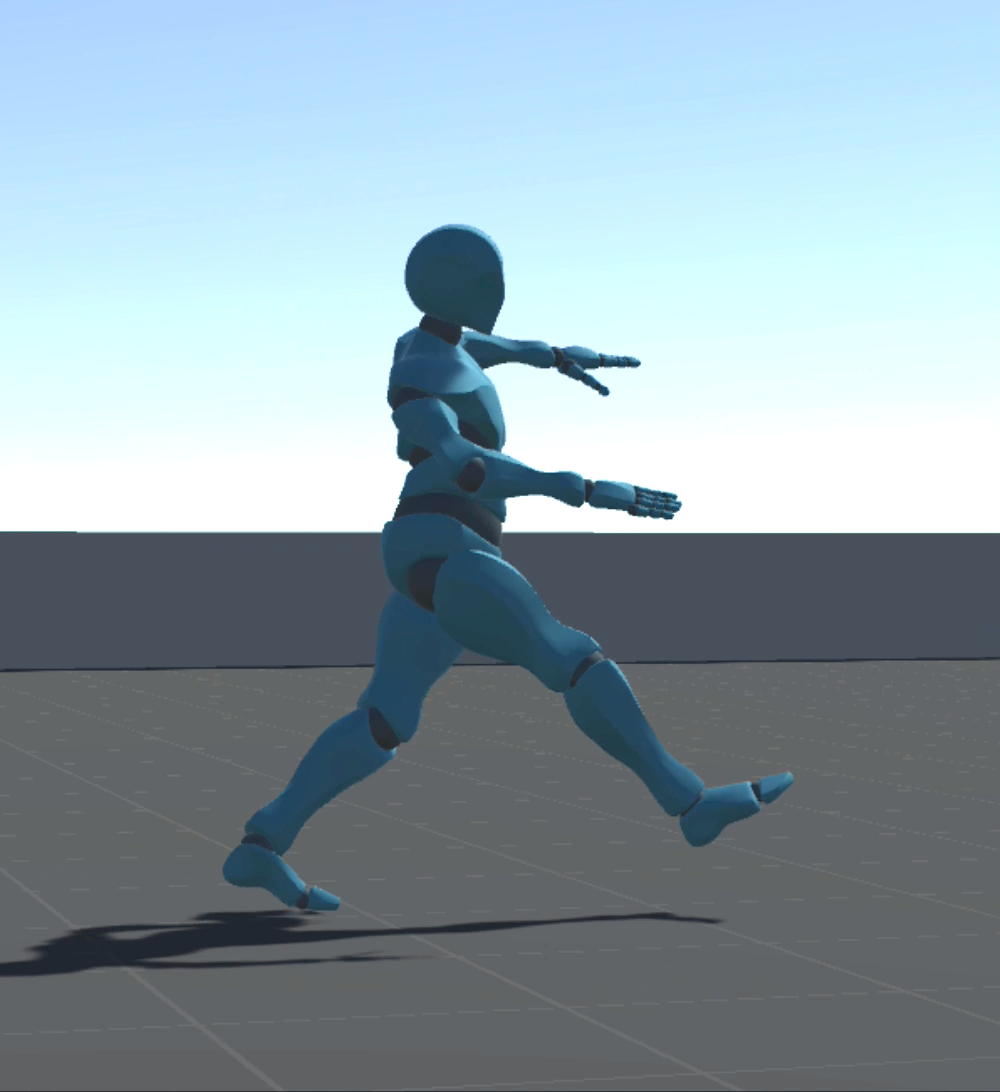
\includegraphics[width=0.27\textwidth]{img/charakter_mixamo_laufen2}  & 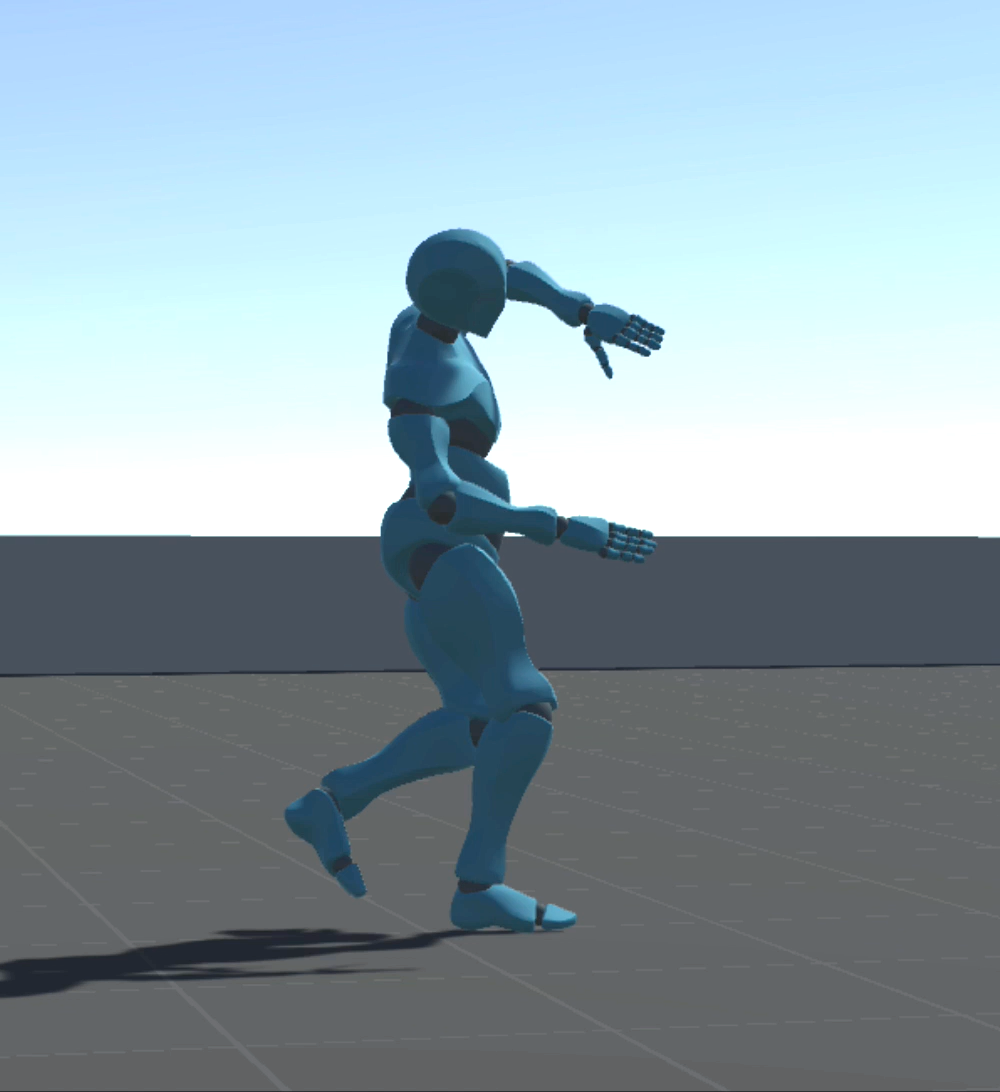
\includegraphics[width=0.27\textwidth]{img/charakter_mixamo_laufen3} \\
    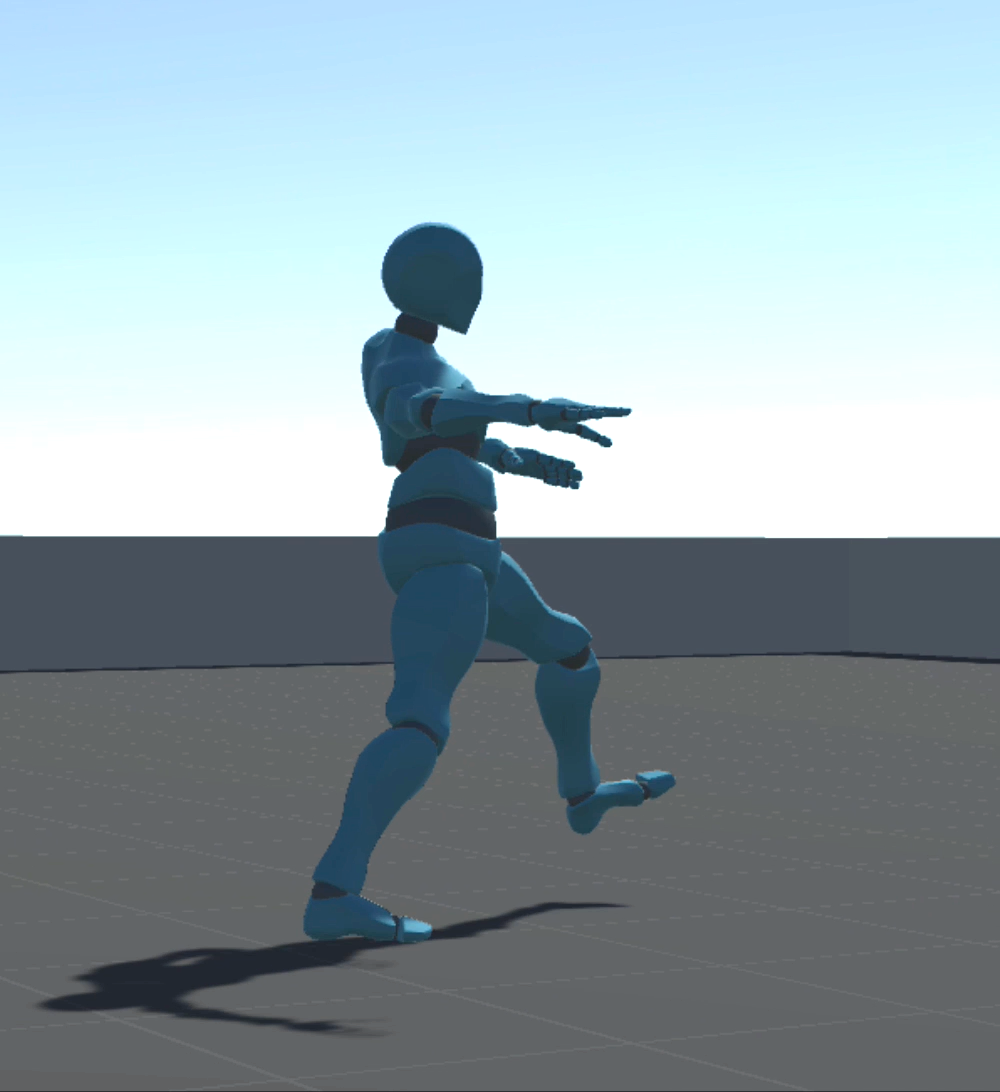
\includegraphics[width=0.27\textwidth]{img/charakter_mixamo_laufen4}  & 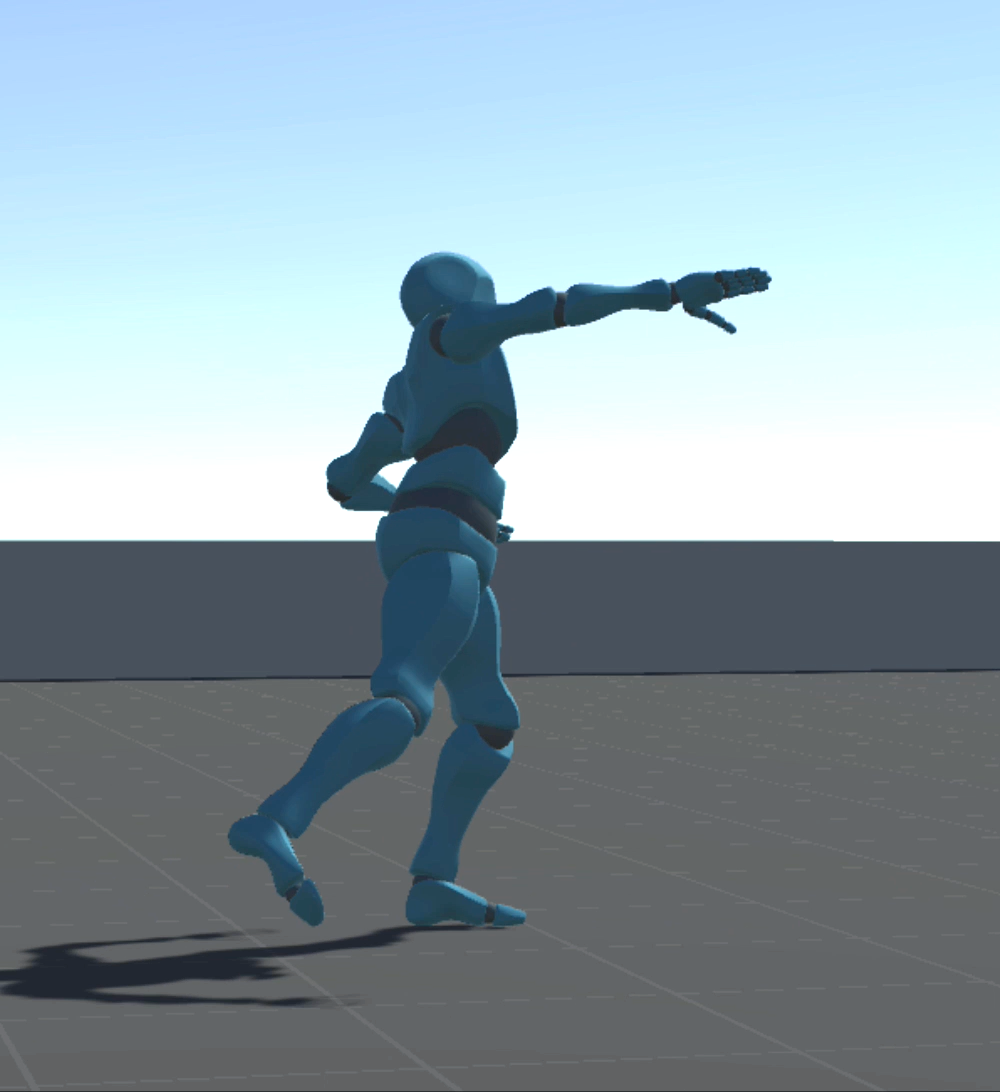
\includegraphics[width=0.27\textwidth]{img/charakter_mixamo_laufen5}  & \includegraphics[width=0.27\textwidth]{img/charakter_mixamo_laufen6} \\
  \end{tabular}
  \caption{Mixamo Charakter Gangbild mit Beinwechselbelohnung}
  \label{fig:mixamo_versuch11_gangbild}
\end{figure}

\newpage
\subsection{Energieminimierung}
Großen Einfluss auf die Entwicklung des menschlichen Gangbilds hat die Energieminimierung. Der Läufer hat keine Wahrnehmung von Aufwand, daher sind die erlernten Bewegungsabläufe oft alles andere als effizient. Um das Gangbild weiter zu verbessern, wird eine Belohnung eingeführt, die den Agenten dafür belohnt, wenn er so wenig wie möglich Kraft aufwendet, um das Ziel zu erreichen. Genauer gesagt wird er dafür bestraft, wenn die Gelenksteuerung einen zu hohen Energiekonsum aufweist. Ähnlich wie die Fußwechselbestrafung wird auch für die Energieminimierung eine Funktion verwendet, bei der die Bestrafung zwischen 150 und 3150 Watt linear ansteigt (siehe Abbildung \ref{fig:plot_energiespar}). Die Wahl der Energie-Schwellenwerte orientiert sich an den im Artikel \grqq{}Assessing the metabolic cost of walking: The influence of baseline subtractions\grqq{} angegebenen durchschnittlichen Energieaufwänden.\cite{5333126}  Für eine Geschwindigkeit von 0,2 m/s bis 1,9 m/s wird ein Energieaufwand von 2,14 bis 6,90 Watt pro kg festgelegt. Mit einem Gewicht des Läufers von 109 kg ergibt sich ein Bereich von 233 bis 752 Watt bei einer vergleichbaren Effizienz. Dieser Bereich ist weit genug gefasst, sodass der Läufer Belohnungen über 0 erreichen kann. Ergebnisse mit steigender Effizienz führen zu nahezu vernachlässigbaren Bestrafungen. Die Funktion ergibt für 233 Watt eine Bestrafung von 0,027 und für 752 Watt eine Bestrafung von 0,2. Aufgrund der variablen Sensitivität der Geschwindigkeitsbelohnungsfunktion erreicht der Läufer selten eine solch hohe Geschwindigkeit, sodass die Bestrafung durch das Optimieren der Gangbewegung nahezu auf 0 reduziert werden kann.

\begin{figure}[H]
  \centering
  \includegraphics[width=0.85\textwidth]{img/plot_energiespar} 
  \caption{Energiesparbelohnung}
  \label{fig:plot_energiespar}
\end{figure}

Die Energieminimierung bringt den Läufer dazu, seine Bewegungen zu optimieren und somit zu minimieren (siehe Abbildung \ref{fig:mixamo_versuch12_gangbild}). Das Gangbild wirkt dadurch natürlicher, insbesondere weil die Bein- und Körperbewegungen wesentlich verbessert wurden. Zuvor hat der Läufer beim Laufen den Oberkörper über das Standbein gekippt, nach der Einführung der Energiesparbelohnung wurde die Oberkörperbewegung minimiert. Allerdings hat die Energieminimierung auch dazu geführt, dass die Arme so gut wie gar nicht mehr bewegt werden. Das Fehlen der Armbewegung tritt im Gesamtbild der natürlichen Bewegung negativ auf.

\begin{figure}[H]
  \centering
  \begin{tabular}{ccc}
    \includegraphics[width=0.27\textwidth]{img/charakter_mixamo_laufen_energiespar1} & \includegraphics[width=0.27\textwidth]{img/charakter_mixamo_laufen_energiespar2}  & \includegraphics[width=0.27\textwidth]{img/charakter_mixamo_laufen_energiespar3} \\
    \includegraphics[width=0.27\textwidth]{img/charakter_mixamo_laufen_energiespar4}  & \includegraphics[width=0.27\textwidth]{img/charakter_mixamo_laufen_energiespar5}  & \includegraphics[width=0.27\textwidth]{img/charakter_mixamo_laufen_energiespar6} \\
  \end{tabular}
  \caption{Mixamo Charakter Gangbild mit Energiesparbelohnung}
  \label{fig:mixamo_versuch12_gangbild}
\end{figure}

\subsection{Armpendel}
Die Arme sind für eine natürliche Gehbewegung unabdinglich. Ein gesunder Mensch bewegt die Arme beim gehen gegensätzlich zu den Beinen. Einige Vermutungen, warum der Mensch dieses Verhalten zeigt, sind die Verbesserung der Stabilität, Energieminimierung oder die Abstammung von Vorfahren, welche die Arme aktiv beim Fortbewegen einsetzten.\cite{meyns2013and}

Der Grund ist für die Entwicklung eines natürlichen Charakterkontrollers jedoch zweitrangig. Durch die vereinfachte physikalische Darstellung muss das für Menschen natürliche Verhalten teilweise über Umwege antrainiert werden. Um die Arme während des Laufens gegensätzlich zu den Beinen zu schwingen, wird die Verwendung einer weiteren Bestrafung getestet. Für die Bestrafung wird die Distanz der Hände, sowie Hüfte zum Ziel berechnet. Abhängig von der führenden Seite (Bein vorne) werden die Werte so aufsummiert, dass bei korrekter Armorientierung ein positiver Wert und gleicherweise bei falscher Armorientierung ein negativer Wert herauskommt. Ist das linke Bein vorne, sieht die Berechnung wie folgt aus: $(hüftdistanz - rechteHandDistanz) + (linkeHandDistanz - hüftDistanz)$ ist das rechte Bein vorne, werden die Hand Distanzen vertauscht und man erhält $(hüftdistanz - linkeHandDistanz) + (rechteHandDistanz - hüftDistanz)$. Die errechnete Distanz wird in Abbildung \ref{fig:pendelsumme_distanz} dargestellt.

\begin{figure}[H]
  \centering  
    \begin{subfigure}{.49\textwidth}
      \centering  
      \includegraphics[width=\textwidth]{img/hand_pendel_gut}
      \caption{Richtige Armpendel Richtung (Distanz positiv)}
      \label{fig:hand_pendel_gut}
    \end{subfigure}
    \begin{subfigure}{.49\textwidth}
      \centering  
      \includegraphics[width=\textwidth]{img/hand_pendel_schlecht}
      \caption{Falsche Armpendel Richtung (Distanz negativ)}
      \label{fig:hand_pendel_schlecht}
    \end{subfigure}
  \caption{Pendelsumme Distanz Veranschaulichung}
  \label{fig:pendelsumme_distanz}
\end{figure}

Anschließend wird die Distanz mit einer Clip ähnlichen Funktion (siehe Abbildung \ref{fig:plot_hand_pendel}) auf einen Bereich von -1 bis 1 beschränkt, abschließend werden die Werte auf einen Bereich von -1 bis 0 skaliert.

\begin{figure}[H]
  \centering  
  \includegraphics[width=0.85\textwidth]{img/plot_hand_pendel}
  \caption{Armpendelbestrafung}
  \label{fig:plot_hand_pendel}
\end{figure}

Die neu eingeführte Armpendel Bestrafung hat nicht die erwarteten Ergebnisse erzielt. Zu Beginn des Trainings dominiert die Bestrafung so stark mit -0,48 Punkten pro Trainingsschritt, dass der Läufer sich entscheidet nur diese Bestrafung zu optimieren und gleichzeitig so schnell wie möglich das frühe Stop auszulösen, um zusätzliche Bestrafung zu verhindern. Um zu evaluieren ob die entwickelte Belohnungsfunktion das gewollte Verhalten verstärkt, muss hier ein Training mit weniger starken Bestrafungen durchgeführt werden.

\subsection{Imitationslernen}
Imitationslernen ist eine weit verbreitete Technik, um Agenten im verstärkenden Lernen ein bestehendes Verhalten anhand von Aufzeichnungen anzutrainieren. Ein Vorteil des Imitationslernens besteht darin, dass natürliche Verhaltensmuster aus der Referenz übernommen werden und somit weniger spezialisierte Belohnungen erforderlich sind. Als Referenz für die Steuerung menschlicher Charaktere werden Bewegungsaufnahmen von Menschen verwendet. Unity ML-Agents bietet für das Imitationslernen zwei Algorithmen an: Behavioral Cloning und Generative Adversarial Imitation Learning. Beide verwenden als Referenz eine aufgenommene Demonstration. Zum Aufnehmen einer Demonstration existiert die Demonstration Recorder Komponente, die auf ein Objekt mit Agent hinzugefügt wird. Anschließend kann das heuristische Verhalten des Agenten aufgezeichnet werden. Im Fall der Läufer-Trainingsumgebung ist es jedoch schwierig, ein solches Verhalten zu entwickeln, da zusätzlich zu den Gelenkrotationen, die aus Bewegungsaufnahmen entnommen werden können, auch die Gelenkstärke benötigt wird. Aufgrund dieser Anforderungen sind die von Unity ML-Agents verfügbaren Systeme für das Imitationslernen in diesem Fall nicht geeignet. Daher wurde das Imitationslernen basierend auf den in der Arbeit \grqq{}DeepMimic: Example-Guided Deep Reinforcement Learning of Physics-Based Character Skills\grqq{} entwickelten Imitationsbelohnungsfunktionen getestet.\cite{peng2018deepmimic} Als Referenzbewegung werden Motion Capture Daten aus der \grqq{}SFU Motion Capture Database\grqq{} genutzt.\cite{sfu-motion-capture}

Zu Beginn einer Trainingsepisode wurde die Referenzanimation zurückgesetzt und der Läufer auf die gleiche Startpose gesetzt. Der Agent erhält zusätzlich zu seiner normalen Beobachtung auch eine Phasenvariable, die die aktuelle Phase der Animation widerspiegelt. Es wurde untersucht, wie sich die Kombination der Körperhaltungsbelohnung (Posereward) aus dem Deep Mimic Artikel mit den Walker Demo Belohnungen auf das Verhalten auswirkt. Die Körperhaltungsbelohnung belohnt die Übereinstimmung der relativen Körperteilrotationen und ist somit positionsunabhängig. Da jedoch die Hüfte bzw. das Hauptkörperteil eines Charakters keine Referenz hat, zu der diese Rotation relativ bestimmt werden kann, wurde eine Ausnahmeregel für die Hüfte entwickelt, die nur die Rotation in zwei Richtungen vergleicht: die X- und Z-Rotation. Die Rotation um die Y-Achse wird ignoriert, um unterschiedliche Orientierungen des Körpers und damit unterschiedliche Zielrichtungen zuzulassen, ohne diese zu bestrafen. Der Läufer entwickelte ein rückwärts übergebeugtes Gehverhalten (siehe Abbildung \ref{fig:charakter_mixamo_imitation}), es ist unklar, ob der Läufer die Referenzbewegung teilweise imitiert hat. Der Auslöser für das merkwürdige Gangbild ist ebenfalls nicht eindeutig. Eine mögliche Ursache könnte ein Fehler im Vergleich der Hüftrotation sein. Teile der Implementierung werden in \ref{code:imitation_belohnung} und \ref{code:animation_init} aufgezeigt.

\begin{figure}[H]
  \centering  
  \includegraphics[width=0.9\textwidth]{img/charakter_mixamo_imitation}
  \caption{Mixamo Charakter Gangbild mit Körperhaltungsbelohnung}
  \label{fig:charakter_mixamo_imitation}
\end{figure}
{\chapter{Fazit}}
\label{sec:fazit}
Text
\appendix

%Literaturverzeichnis
\printbibliography[title=Literaturverzeichnis]

\end{document}